\usepackage{ifthen}
\usepackage{graphicx}
\usepackage{booktabs}
\usepackage{tabularx}
\usepackage{algorithm}
%\usepackage{algorithmx}
%\usepackage{cwpuzzle}
\usepackage{algpseudocode}
\usepackage[english]{babel}
%\usepackage{qtree}
\usepackage{amssymb}
\usepackage{amsmath,amsthm}
\usepackage{subcaption}
\usepackage{mathrsfs}
%\usepackage{eurosym}
\usepackage{soul}
\usepackage{fontawesome}
\usepackage{etoolbox}
\usepackage{soul}
\usepackage{multicol}
\usepackage{listings}
\usepackage{color}

\definecolor{mygreen}{rgb}{0,0.6,0}
\definecolor{mygray}{rgb}{0.5,0.5,0.5}
\definecolor{mymauve}{rgb}{0.58,0,0.82}
\usepackage{tikz}
\usepackage{xstring}
\usepackage{pgfplots}
\usepackage{etoolbox}
\usepackage{ifthen}
\usetikzlibrary{arrows,shapes}
\usetikzlibrary{positioning, calc}

\definecolor{hospital}{RGB}{0,0,255}
\definecolor{patient}{RGB}{255,0,0}

\tikzstyle{flow_node}=[circle,draw=black,minimum size=15pt,inner sep=0pt]
\tikzstyle{flow_s}=[fill=green!20]
\tikzstyle{flow_subtask}=[fill=green!80]
\tikzstyle{flow_task}=[fill=red!80]
\tikzstyle{flow_t}=[fill=blue!20]
\tikzstyle{flow_edge}=[->, ultra thick]
\tikzstyle{flow_capacity}=[fill=white, inner sep = 1pt]
\tikzstyle{flow_edge_mincut}=[draw=red]
\tikzstyle{flow_edge_fullcap}=[draw=red]
\tikzstyle{flow_mincut}=[dashed, thick]
\tikzstyle{flow_supply}=[fill=green!80]
\tikzstyle{flow_demand}=[fill=red!80]

\newcommand\ifMaxFlow[4]{
	\begingroup
		\pgfmathsetmacro{\flow}{#1}
		\pgfmathsetmacro{\cap}{#2}
		\pgfmathparse{ifthenelse(\flow == \cap,1,0)}
		\ifdim\pgfmathresult pt= 1 pt
			 #3
			\else
			 #4
		\fi
	\endgroup
}

\newcommand\ifSomeFlow[3]{
	\begingroup
		\pgfmathsetmacro{\flow}{#1}
		\pgfmathparse{ifthenelse(\flow > 0,1,0)}
		\ifdim\pgfmathresult pt= 1 pt
			 #2
			\else
			 #3
		\fi
	\endgroup
}


\usepackage[duration=105,lastminutes=15]{../common/pdfpcnotes}

\makeatletter
\let\@@magyar@captionfix\relax
\makeatother

\newcommand{\bigO}{O}

\usetheme[width=0mm]{PaloAlto}
\setbeamertemplate{navigation symbols}
{\ifthenelse{\not\equal{\thepage}{1}}
  {\insertframenumber}
  {}
}
\setbeamertemplate{footline}%
{\ifthenelse{\not\equal{\thepage}{1}}%
  {\color{gray!30!white}{\tiny \copyright 2018 TU Delft}}% \hfill\insertframenumber/\inserttotalframenumber}
  {}
}

\newenvironment<>{problemblock}[1]{%
  \begin{actionenv}#2%
      \def\insertblocktitle{Problem: #1}%
      \par%
      \mode<presentation>{%
        \setbeamercolor{block title}{fg=white,bg=orange!80!black}
       \setbeamercolor{block body}{fg=black,bg=orange!40}
       \setbeamercolor{itemize item}{fg=orange!20!black}
       \setbeamertemplate{itemize item}[triangle]
     }%
      \usebeamertemplate{block begin}}
    {\par\usebeamertemplate{block end}\end{actionenv}}

\newenvironment<>{questionblock}[1]{%
  \begin{actionenv}#2%
      \def\insertblocktitle{Question: #1}%
      \par%
      \mode<presentation>{%
        \setbeamercolor{block title}{fg=white,bg=cyan!80!black}
       \setbeamercolor{block body}{fg=black,bg=cyan!30}
       \setbeamercolor{itemize item}{fg=cyan!20!black}
       \setbeamertemplate{itemize item}[triangle]
     }%
      \usebeamertemplate{block begin}}
    {\par\usebeamertemplate{block end}\end{actionenv}}

\newenvironment<>{answerblock}[1]{%
  \begin{actionenv}#2%
      \def\insertblocktitle{Answer: #1}%
      \par%
      \mode<presentation>{%
        \setbeamercolor{block title}{fg=white,bg=green!80!black}
       \setbeamercolor{block body}{fg=black,bg=green!30}
       \setbeamercolor{itemize item}{fg=green!20!black}
       \setbeamertemplate{itemize item}[triangle]
     }%
      \usebeamertemplate{block begin}}
    {\par\usebeamertemplate{block end}\end{actionenv}}

% Fix a bug in lstlinebgrd
% https://tex.stackexchange.com/questions/451532/recent-issues-with-lstlinebgrd-package-with-listings-after-the-latters-updates

\makeatletter
\let\old@lstKV@SwitchCases\lstKV@SwitchCases
\def\lstKV@SwitchCases#1#2#3{}
\makeatother
\usepackage{lstlinebgrd}
\makeatletter
\let\lstKV@SwitchCases\old@lstKV@SwitchCases

\lst@Key{numbers}{none}{%
    \def\lst@PlaceNumber{\lst@linebgrd}%
    \lstKV@SwitchCases{#1}%
    {none:\\%
     left:\def\lst@PlaceNumber{\llap{\normalfont
                \lst@numberstyle{\thelstnumber}\kern\lst@numbersep}\lst@linebgrd}\\%
     right:\def\lst@PlaceNumber{\rlap{\normalfont
                \kern\linewidth \kern\lst@numbersep
                \lst@numberstyle{\thelstnumber}}\lst@linebgrd}%
    }{\PackageError{Listings}{Numbers #1 unknown}\@ehc}}
\makeatother

\lstset{ 
  backgroundcolor=\color{white},   % choose the background color; you must add \usepackage{color} or \usepackage{xcolor}; should come as last argument
  basicstyle=\footnotesize\ttfamily,        % the size of the fonts that are used for the code
  breakatwhitespace=false,         % sets if automatic breaks should only happen at whitespace
  breaklines=true,                 % sets automatic line breaking
  captionpos=b,                    % sets the caption-position to bottom
  commentstyle=\color{mygreen},    % comment style
  deletekeywords={...},            % if you want to delete keywords from the given language
	escapeinside={\%*}{*\%},          % if you want to add LaTeX within your code
  extendedchars=true,              % lets you use non-ASCII characters; for 8-bits encodings only, does not work with UTF-8
  frame=single,	                   % adds a frame around the code
  keepspaces=true,                 % keeps spaces in text, useful for keeping indentation of code (possibly needs columns=flexible)
  keywordstyle=\color{blue},       % keyword style
  language=Python,                 % the language of the code
	literate={\ \ }{{\ }}1,					 % Replace two spaces with just one
  morekeywords={*,...},            % if you want to add more keywords to the set
  numbers=left,                    % where to put the line-numbers; possible values are (none, left, right)
  numbersep=5pt,                   % how far the line-numbers are from the code
  numberstyle=\tiny\color{mygray}, % the style that is used for the line-numbers
  rulecolor=\color{black},         % if not set, the frame-color may be changed on line-breaks within not-black text (e.g. comments (green here))
  showspaces=false,                % show spaces everywhere adding particular underscores; it overrides 'showstringspaces'
  showstringspaces=false,          % underline spaces within strings only
  showtabs=false,                  % show tabs within strings adding particular underscores
  stepnumber=1,                    % the step between two line-numbers. If it's 1, each line will be numbered
  stringstyle=\color{mymauve},     % string literal style
  tabsize=2,   	                   % sets default tabsize to 2 spaces
	emptylines=*1
}
\lstset{
	defaultdialect=[LaTeX]TeX
}

%%%%%%%%%%%%%%%%%%%%%%%%%%%%%%%%%%%%%%%%%%%%%%%%%%%%%%%%%%%%%%%%%%%%%%%%%%%%%%%%
% Hacks for highlighting lines in listings, thanks to Robbert Krebbers
%%%%%%%%%%%%%%%%%%%%%%%%%%%%%%%%%%%%%%%%%%%%%%%%%%%%%%%%%%%%%%%%%%%%%%%%%%%%%%%%

\makeatletter
\newlength\beamerleftmargin
\setlength\beamerleftmargin{\Gm@lmargin}
\makeatother

\makeatletter
\newcount\bt@rangea
\newcount\bt@rangeb

\newcommand\btIfInRange[2]{%
    \global\let\bt@inrange\@secondoftwo%
    \edef\bt@rangelist{#2}%
    \foreach \range in \bt@rangelist {%
        \afterassignment\bt@getrangeb%
        \bt@rangea=0\range\relax%
        \pgfmathtruncatemacro\result{ ( #1 >= \bt@rangea) && (#1 <= \bt@rangeb) }%
        \ifnum\result=1\relax%
            \breakforeach%
            \global\let\bt@inrange\@firstoftwo%
        \fi%
    }%
    \bt@inrange%
}
\newcommand\bt@getrangeb{%
    \@ifnextchar\relax%
        {\bt@rangeb=\bt@rangea}%
        {\@getrangeb}%
}
\def\@getrangeb-#1\relax{%
    \ifx\relax#1\relax%
        \bt@rangeb=100000%   \maxdimen is too large for pgfmath
    \else%
        \bt@rangeb=#1\relax%
    \fi%
}

\newcommand<>{\btLstHL}[1]{%
  \only#2{\btIfInRange{\value{lstnumber}}{#1}%
    {\color{blue!30}}%
    {\def\lst@linebgrdcmd####1####2####3{}}% define as no-op
  }%
}%
\makeatother



\title[Algorithms \& Data Structures]{TI1520TW Algorithms \& Data Structures}
\subtitle{\color{cyan} \textbf{Lecture 3: More recursion \& The Master Theorem}}
\author{Stefan Hugtenburg\\ {\tiny{\qquad~~\copyright 2019 TU Delft}}}
\institute{CSE Teaching Team | EEMCS | TU Delft}
\titlegraphic{
\includegraphics[height=1cm]{../common/logo.pdf}~\hfill~
\includegraphics[height=1cm]{../common/cc-by-nc-sa.png}}
\date{2018-2019 Q3}

\begin{document}

\frame{\titlepage}

\section{Introduction}

\begin{frame}
	\frametitle{You are here.}
	\begin{block}{The course so far}
		\begin{itemize}
			\item Time and Space complexity
			\item Lists, Stacks, and Queues
			\item Sorting
		\end{itemize}
	\end{block}
	\pause
	\begin{exampleblock}{Today's content}
		\begin{itemize}
			\item Trees!
			\item Properties and traversals
		\end{itemize}
	\end{exampleblock}
	\pause
	\begin{block}{The future}
		\begin{itemize}
			\item Heaps and Search Trees
			\item Maps, Sets, and Graphs
			\item P vs NP\dots
		\end{itemize}
	\end{block}
\end{frame}


\begin{frame}
	\frametitle{Some small updates}
	\begin{itemize}
		\item Grading of week 1. Sorry we were so late!
		\item We hope to be a lot earlier this week!
			\pause
		\item I will try to generate hand-out versions of my slides as well (less clicking/scrolling).
		\item My slides always end with what sections of the book they correspond to :)
			\pause
		\item FBF fixed the broken links, but now other stuff seems to be broken..
			\pause
		\item You have only a few more days to register for the exams!
		\item Two practice exams will be available by the end of the week (one analysis, one implementation).
			\pause
		\item Again, remember that you can render TeX in WebLab.
	\end{itemize}
\end{frame}

\section{Recursion}
\label{sec:recursion}

\begin{frame}
	\frametitle{WHY!?}
	\framesubtitle{On the topic of recursion}
\begin{center}
	
\includegraphics[width=0.8\textwidth]{figures/why.png}\\
	\hspace*{15pt}\hbox{\scriptsize Image from Pixabay}
	%https://pixabay.com/en/why-text-question-marketing-office-1780726/
\end{center}	
\end{frame}

\begin{frame}
	\frametitle{Why use recursion?}
	\begin{questionblock}{Why?}
		Why might we like to use recursion to solve some problems?
	\end{questionblock}
	\pause
	\begin{answerblock}{}
		\small
		\begin{itemize}
			\item In ``Discrete Mathematics with Applications'' (a book we used to use in Computer Science), the author
				describes recursion as: ``one of the central ideas in computer science''.
			\pause
			\vspace{-5pt}
			\item A nice (mathematical?) construct: problems can often be reduced to smaller sub problems.
			\pause
			\vspace{-5pt}
			\item Parallelisation: make one problem two smaller problems that separate computers can solve.
		\end{itemize}	
	\end{answerblock}
	\pause
		\begin{alertblock}{So should we use it for everything? No!}
			\small
			In the homework, we force you to use it on problems where iteration makes more sense.\\
			This is unfortunate, but needed to practice.
		\end{alertblock}	
\end{frame}



\section{Closest pair of points}
\label{sec:closest_pair_of_points}


\begin{frame}
	\frametitle{A new problem}
	\begin{problemblock}{Closest pair of points}
		Given a set of points, what is the pair of points that is closest to each other?\\
		\pause
		More formally:
		\begin{itemize}
			\item Given a set of points $S$, where every point $p_i$ has an x-coordinate $x_i$ and y-coordinate $y_i$.
			\item Distance is defined as: $d(i,j) = \sqrt{{(x_i - x_j)}^{2} + {(y_i-y_j)}^2}$
			\item What is the pair of points $i,j$ such that $d(i,j)$ is minimal?
		\end{itemize}
	\end{problemblock}
	\pause
	\section{Closest pair of points}
\label{sec:closest_pair_of_points}


\begin{frame}
	\frametitle{A new problem}
	\begin{problemblock}{Closest pair of points}
		Given a set of points, what is the pair of points that is closest to each other?\\
		\pause
		More formally:
		\begin{itemize}
			\item Given a set of points $S$, where every point $p_i$ has an x-coordinate $x_i$ and y-coordinate $y_i$.
			\item Distance is defined as: $d(i,j) = \sqrt{{(x_i - x_j)}^{2} + {(y_i-y_j)}^2}$
			\item What is the pair of points $i,j$ such that $d(i,j)$ is minimal?
		\end{itemize}
	\end{problemblock}
	\pause
	\section{Closest pair of points}
\label{sec:closest_pair_of_points}


\begin{frame}
	\frametitle{A new problem}
	\begin{problemblock}{Closest pair of points}
		Given a set of points, what is the pair of points that is closest to each other?\\
		\pause
		More formally:
		\begin{itemize}
			\item Given a set of points $S$, where every point $p_i$ has an x-coordinate $x_i$ and y-coordinate $y_i$.
			\item Distance is defined as: $d(i,j) = \sqrt{{(x_i - x_j)}^{2} + {(y_i-y_j)}^2}$
			\item What is the pair of points $i,j$ such that $d(i,j)$ is minimal?
		\end{itemize}
	\end{problemblock}
	\pause
	\input{figures/tikz/closestpair.tex}
	\pnote{Why is this relevant? Answers: For instance collision detection algorithms}
\end{frame}

\begin{frame}
	\frametitle{Let's just brute-force it?}
	\begin{overlayarea}{\textwidth}{\textheight}
		\input{figures/tikz/closestpair.tex}
		\begin{questionblock}{Brute-force}
			What is the tightest upper bound on the run time for a brute-force solution given $|S| = n$?
			\only<2>{
			\begin{enumerate}[A.]
				\item $O(n \log n)$
				\item $O(n^2)$
				\item $O(n^2 \log n)$
				\item $O(n^3)$
				\item I don't know.
			\end{enumerate}
		}
		\end{questionblock}
		\only<3>{
			\begin{answerblock}{Try every combination}
				We check every pair of points, of which there are $n^2$, so $O(n^2)$.	
			\end{answerblock}
		}
	\end{overlayarea}
\end{frame}

\begin{frame}
	\frametitle{Time to improve!}
	\framesubtitle{Using Divide \& Conquer}
		\begin{columns}
			\column{0.455\textwidth}
			\begin{center}
				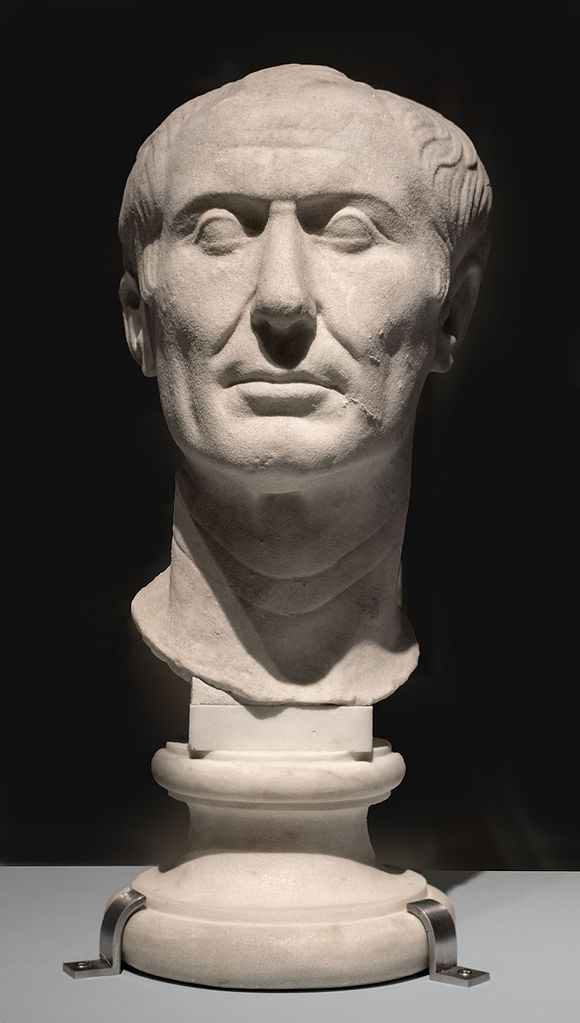
\includegraphics[width=0.5\textwidth]{figures/ceasar.jpg}\\
				\hspace*{15pt}\hbox{\scriptsize Image By:\thinspace{\itshape Ángel M. Felicísimo}}
				%https://commons.wikimedia.org/wiki/File:Retrato_de_Julio_C%C3%A9sar_(26724093101).jpg
			\end{center}

			\column{0.455\textwidth}
			\begin{center}
				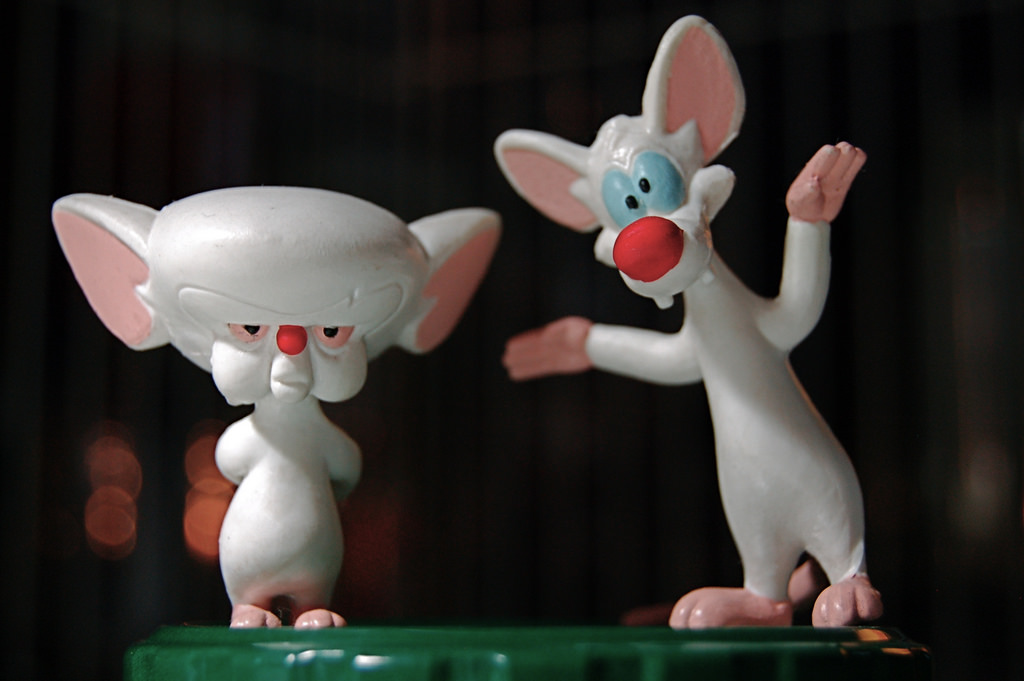
\includegraphics[width=0.9\textwidth]{figures/pinky.jpg}\\
				\hspace*{15pt}\hbox{\scriptsize Image By:\thinspace{\itshape JD Hancock}}
				%https://commons.wikimedia.org/wiki/File:Retrato_de_Julio_C%C3%A9sar_(26724093101).jpg

			\end{center}
		\end{columns}
\end{frame}

\begin{frame}
	\frametitle{Ideas for an algorithm}

	\begin{overlayarea}{\textwidth}{\textheight}
		\input{figures/tikz/closestpair_fixed.tex}
		
		\pause
		\begin{exampleblock}{Algorithm}
			\begin{itemize}
				\item \alert<2>{Divide}: Draw vertical line $L$ that has roughly half of the points on each side.
					\pause
				\item \alert<3>{Conquer}: Find the closest pair on each side.
					\pause
				\item \alert<4>{Combine}: Find the closest pair with one point on each side.
					\pause
				\item Return the minimum of these 3.
			\end{itemize}
		\end{exampleblock}	
	\end{overlayarea}
\end{frame}

\begin{frame}
	\frametitle{Did we make things better?}
	\begin{questionblock}{What is the run time of combine?}
		How much time to combine the two halves? Remember that we want to improve over $\Theta(n^2)$.
	\end{questionblock}	
\end{frame}

\begin{frame}
	\frametitle{How do we make it better?}
		\input{figures/tikz/closestpair_fixed2.tex}
	Observation:
	\begin{itemize}
		\item If $\delta$ is the minimum of the smallest distances left and right.
			\pause
		\item Then we only need to consider pairs of points within $\delta$ of $L$.
			\pause
		\item So in this example, none at all!
	\end{itemize}
\end{frame}

\begin{frame}
	\frametitle{Worst-case?}
	\begin{overlayarea}{\textwidth}{\textheight}
			\begin{itemize}
				\item But worst-case all points are in this $2\delta$-strip...
					\pause
				\item But if we sort them by $y$-coordinate (which can be done in $O(n\log n)$), then how many comparisons do we need?
					\pause
				\item Still $O(n^2)$!?
					\only<4->{
				\item Nope! We only need to check within 11 (i.e. a constant number of) positions in the sorted list.
				}
					\only<5->{
				\item So the combining step is $O(n \log n)$ (which can be further improved to $O(n)$)!
				}
			\end{itemize}
			\only<3>{
			\begin{center}
				
\includegraphics[width=0.4\textwidth]{figures/dilbert.jpg}
				\framesubtitle{http://thecontextofthings.com/wp-content/uploads/2017/11/dilbert-work.jpg}
			\end{center}
		}
	\end{overlayarea}
\end{frame}

\begin{frame}
	\frametitle{Why 11?}

	\begin{overlayarea}{\textwidth}{\textheight}
		\begin{columns}
			\column{0.655\textwidth}
			\begin{block}{Definition}
				Let $s_i$ be the point in the $2\delta$-strip with the $i^\text{th}$ smallest $y$-coordinate.
			\end{block}	
			
			\pause
			\begin{block}{Claim about 11}
				If $|i-j| > 11$ then the distance between $s_i$ and $s_j$ is at least $\delta$.
			\end{block}
			\column{0.255\textwidth}
			\input{figures/tikz/closestpair_delta.tex}	
		\end{columns}
		
		\pause
		\only<3-5>{
			\begin{block}{Proof sketch}
			\begin{itemize}
				\item No two points are in the same $0.5\delta$-by-$0.5\delta$-box.
					\only<4->{
				\item Two points that have two rows between them have a distance $\geq 2\cdot(0.5\delta) = \delta$.
				}
				\only<5->{
				\item So we only consider points at most 2 rows away.
				}
			\end{itemize}
		\end{block}
	}
	\only<6->{
		\begin{exampleblock}{Fun facts!}
			\begin{itemize}
				\item We can even reduce this to just 7 points.
					\only<7>{
				\item Even less if we consider columns separately.
				}
			\end{itemize}
		\end{exampleblock}	
	}
		
		\only<3>{
		\begin{questionblock}{Why not?}
			Why are there no two points in the same box?
		\end{questionblock}
}
	\end{overlayarea}
\end{frame}

\begin{frame}
	\frametitle{The algorithm}
	\begin{columns}
		\column{0.705\textwidth}
	\begin{algorithmic}
		\State Sort all points by x-coordinate
		\Function{Closest-Pair}{$p_1,\dots,p_n$}
			\If{n=1}
				\State \Return $\infty$
			\EndIf

			\pause
			\State $L \gets$ \alert<2>{median} $x$-coordinate
			\State $\delta_1 \gets$ \Call{Closest-Pair}{Points left of $L$}
			\State $\delta_2 \gets$ \Call{Closest-Pair}{Points right of $L$}
			\State $\delta \gets \min(\delta_1,\delta_2)$
			\pause
			\State get list of all points within $\delta$ from L.
			\State sort this list by y-coordinate
			\pause
			\State Scan by y-order, compare every point to the next 11 and update $\delta$ as you go.
			\State \Return $\delta$
		\EndFunction
	\end{algorithmic}
		\pnote{Why not the average?}
		\column{0.205\textwidth}
		\pause
		\begin{questionblock}{}
			What is the recurrence equation for the run time?	
		\end{questionblock}	
		\pause
		\begin{answerblock}{}
			\small
			$T(n) =2T(n/2) + O(n\log n)$	
		\end{answerblock}
	\end{columns}
	
\end{frame}

	\pnote{Why is this relevant? Answers: For instance collision detection algorithms}
\end{frame}

\begin{frame}
	\frametitle{Let's just brute-force it?}
	\begin{overlayarea}{\textwidth}{\textheight}
		\section{Closest pair of points}
\label{sec:closest_pair_of_points}


\begin{frame}
	\frametitle{A new problem}
	\begin{problemblock}{Closest pair of points}
		Given a set of points, what is the pair of points that is closest to each other?\\
		\pause
		More formally:
		\begin{itemize}
			\item Given a set of points $S$, where every point $p_i$ has an x-coordinate $x_i$ and y-coordinate $y_i$.
			\item Distance is defined as: $d(i,j) = \sqrt{{(x_i - x_j)}^{2} + {(y_i-y_j)}^2}$
			\item What is the pair of points $i,j$ such that $d(i,j)$ is minimal?
		\end{itemize}
	\end{problemblock}
	\pause
	\input{figures/tikz/closestpair.tex}
	\pnote{Why is this relevant? Answers: For instance collision detection algorithms}
\end{frame}

\begin{frame}
	\frametitle{Let's just brute-force it?}
	\begin{overlayarea}{\textwidth}{\textheight}
		\input{figures/tikz/closestpair.tex}
		\begin{questionblock}{Brute-force}
			What is the tightest upper bound on the run time for a brute-force solution given $|S| = n$?
			\only<2>{
			\begin{enumerate}[A.]
				\item $O(n \log n)$
				\item $O(n^2)$
				\item $O(n^2 \log n)$
				\item $O(n^3)$
				\item I don't know.
			\end{enumerate}
		}
		\end{questionblock}
		\only<3>{
			\begin{answerblock}{Try every combination}
				We check every pair of points, of which there are $n^2$, so $O(n^2)$.	
			\end{answerblock}
		}
	\end{overlayarea}
\end{frame}

\begin{frame}
	\frametitle{Time to improve!}
	\framesubtitle{Using Divide \& Conquer}
		\begin{columns}
			\column{0.455\textwidth}
			\begin{center}
				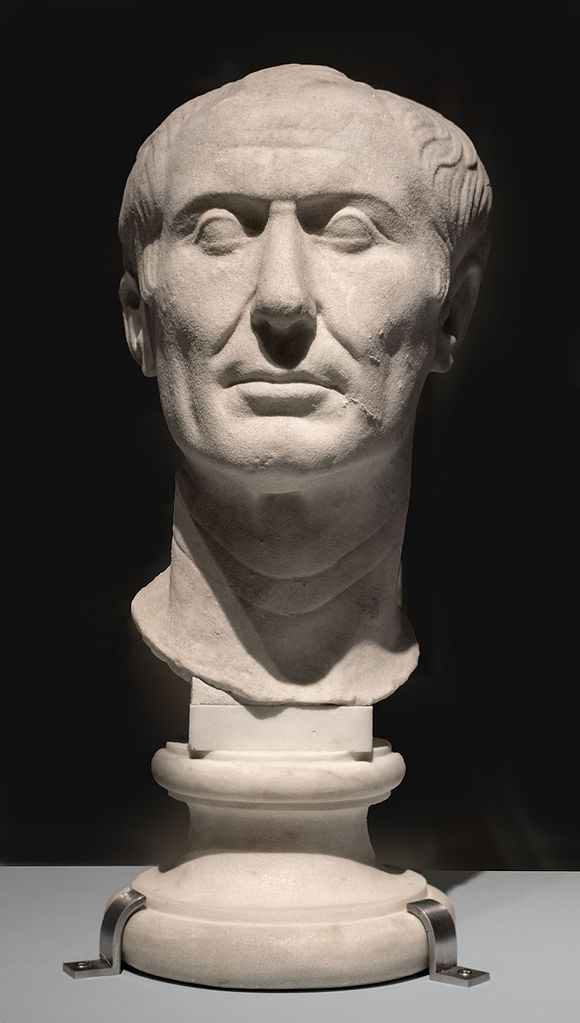
\includegraphics[width=0.5\textwidth]{figures/ceasar.jpg}\\
				\hspace*{15pt}\hbox{\scriptsize Image By:\thinspace{\itshape Ángel M. Felicísimo}}
				%https://commons.wikimedia.org/wiki/File:Retrato_de_Julio_C%C3%A9sar_(26724093101).jpg
			\end{center}

			\column{0.455\textwidth}
			\begin{center}
				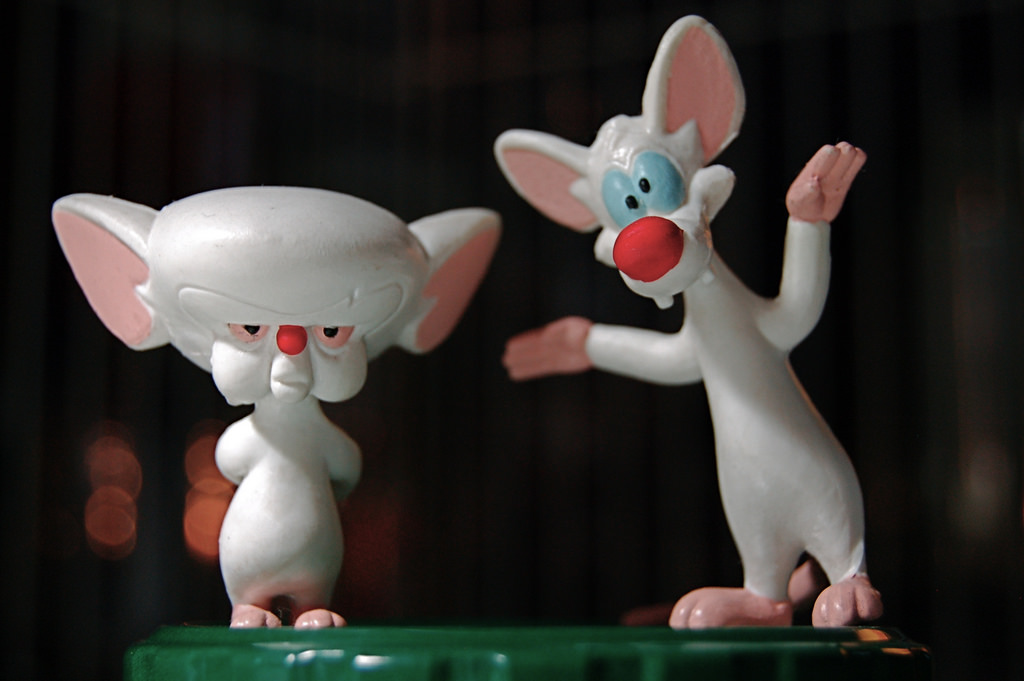
\includegraphics[width=0.9\textwidth]{figures/pinky.jpg}\\
				\hspace*{15pt}\hbox{\scriptsize Image By:\thinspace{\itshape JD Hancock}}
				%https://commons.wikimedia.org/wiki/File:Retrato_de_Julio_C%C3%A9sar_(26724093101).jpg

			\end{center}
		\end{columns}
\end{frame}

\begin{frame}
	\frametitle{Ideas for an algorithm}

	\begin{overlayarea}{\textwidth}{\textheight}
		\input{figures/tikz/closestpair_fixed.tex}
		
		\pause
		\begin{exampleblock}{Algorithm}
			\begin{itemize}
				\item \alert<2>{Divide}: Draw vertical line $L$ that has roughly half of the points on each side.
					\pause
				\item \alert<3>{Conquer}: Find the closest pair on each side.
					\pause
				\item \alert<4>{Combine}: Find the closest pair with one point on each side.
					\pause
				\item Return the minimum of these 3.
			\end{itemize}
		\end{exampleblock}	
	\end{overlayarea}
\end{frame}

\begin{frame}
	\frametitle{Did we make things better?}
	\begin{questionblock}{What is the run time of combine?}
		How much time to combine the two halves? Remember that we want to improve over $\Theta(n^2)$.
	\end{questionblock}	
\end{frame}

\begin{frame}
	\frametitle{How do we make it better?}
		\input{figures/tikz/closestpair_fixed2.tex}
	Observation:
	\begin{itemize}
		\item If $\delta$ is the minimum of the smallest distances left and right.
			\pause
		\item Then we only need to consider pairs of points within $\delta$ of $L$.
			\pause
		\item So in this example, none at all!
	\end{itemize}
\end{frame}

\begin{frame}
	\frametitle{Worst-case?}
	\begin{overlayarea}{\textwidth}{\textheight}
			\begin{itemize}
				\item But worst-case all points are in this $2\delta$-strip...
					\pause
				\item But if we sort them by $y$-coordinate (which can be done in $O(n\log n)$), then how many comparisons do we need?
					\pause
				\item Still $O(n^2)$!?
					\only<4->{
				\item Nope! We only need to check within 11 (i.e. a constant number of) positions in the sorted list.
				}
					\only<5->{
				\item So the combining step is $O(n \log n)$ (which can be further improved to $O(n)$)!
				}
			\end{itemize}
			\only<3>{
			\begin{center}
				
\includegraphics[width=0.4\textwidth]{figures/dilbert.jpg}
				\framesubtitle{http://thecontextofthings.com/wp-content/uploads/2017/11/dilbert-work.jpg}
			\end{center}
		}
	\end{overlayarea}
\end{frame}

\begin{frame}
	\frametitle{Why 11?}

	\begin{overlayarea}{\textwidth}{\textheight}
		\begin{columns}
			\column{0.655\textwidth}
			\begin{block}{Definition}
				Let $s_i$ be the point in the $2\delta$-strip with the $i^\text{th}$ smallest $y$-coordinate.
			\end{block}	
			
			\pause
			\begin{block}{Claim about 11}
				If $|i-j| > 11$ then the distance between $s_i$ and $s_j$ is at least $\delta$.
			\end{block}
			\column{0.255\textwidth}
			\input{figures/tikz/closestpair_delta.tex}	
		\end{columns}
		
		\pause
		\only<3-5>{
			\begin{block}{Proof sketch}
			\begin{itemize}
				\item No two points are in the same $0.5\delta$-by-$0.5\delta$-box.
					\only<4->{
				\item Two points that have two rows between them have a distance $\geq 2\cdot(0.5\delta) = \delta$.
				}
				\only<5->{
				\item So we only consider points at most 2 rows away.
				}
			\end{itemize}
		\end{block}
	}
	\only<6->{
		\begin{exampleblock}{Fun facts!}
			\begin{itemize}
				\item We can even reduce this to just 7 points.
					\only<7>{
				\item Even less if we consider columns separately.
				}
			\end{itemize}
		\end{exampleblock}	
	}
		
		\only<3>{
		\begin{questionblock}{Why not?}
			Why are there no two points in the same box?
		\end{questionblock}
}
	\end{overlayarea}
\end{frame}

\begin{frame}
	\frametitle{The algorithm}
	\begin{columns}
		\column{0.705\textwidth}
	\begin{algorithmic}
		\State Sort all points by x-coordinate
		\Function{Closest-Pair}{$p_1,\dots,p_n$}
			\If{n=1}
				\State \Return $\infty$
			\EndIf

			\pause
			\State $L \gets$ \alert<2>{median} $x$-coordinate
			\State $\delta_1 \gets$ \Call{Closest-Pair}{Points left of $L$}
			\State $\delta_2 \gets$ \Call{Closest-Pair}{Points right of $L$}
			\State $\delta \gets \min(\delta_1,\delta_2)$
			\pause
			\State get list of all points within $\delta$ from L.
			\State sort this list by y-coordinate
			\pause
			\State Scan by y-order, compare every point to the next 11 and update $\delta$ as you go.
			\State \Return $\delta$
		\EndFunction
	\end{algorithmic}
		\pnote{Why not the average?}
		\column{0.205\textwidth}
		\pause
		\begin{questionblock}{}
			What is the recurrence equation for the run time?	
		\end{questionblock}	
		\pause
		\begin{answerblock}{}
			\small
			$T(n) =2T(n/2) + O(n\log n)$	
		\end{answerblock}
	\end{columns}
	
\end{frame}

		\begin{questionblock}{Brute-force}
			What is the tightest upper bound on the run time for a brute-force solution given $|S| = n$?
			\only<2>{
			\begin{enumerate}[A.]
				\item $O(n \log n)$
				\item $O(n^2)$
				\item $O(n^2 \log n)$
				\item $O(n^3)$
				\item I don't know.
			\end{enumerate}
		}
		\end{questionblock}
		\only<3>{
			\begin{answerblock}{Try every combination}
				We check every pair of points, of which there are $n^2$, so $O(n^2)$.	
			\end{answerblock}
		}
	\end{overlayarea}
\end{frame}

\begin{frame}
	\frametitle{Time to improve!}
	\framesubtitle{Using Divide \& Conquer}
		\begin{columns}
			\column{0.455\textwidth}
			\begin{center}
				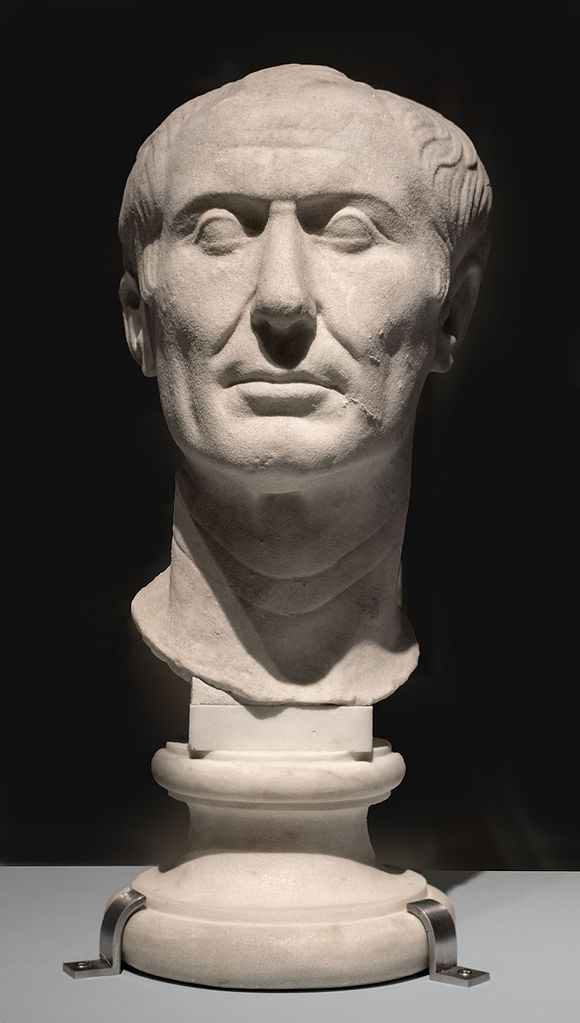
\includegraphics[width=0.5\textwidth]{figures/ceasar.jpg}\\
				\hspace*{15pt}\hbox{\scriptsize Image By:\thinspace{\itshape Ángel M. Felicísimo}}
				%https://commons.wikimedia.org/wiki/File:Retrato_de_Julio_C%C3%A9sar_(26724093101).jpg
			\end{center}

			\column{0.455\textwidth}
			\begin{center}
				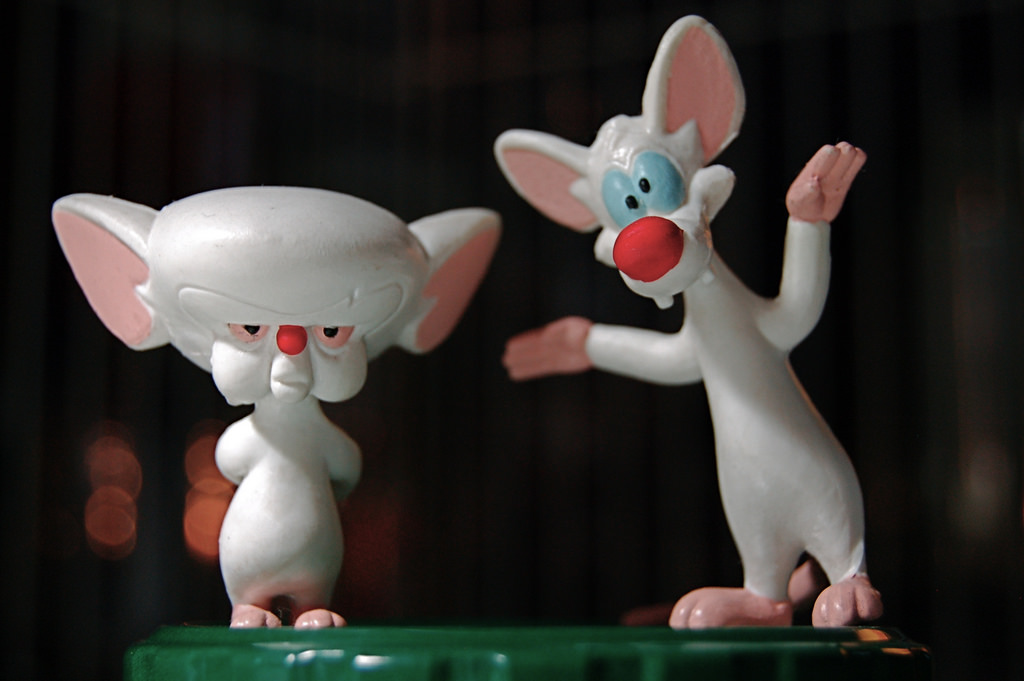
\includegraphics[width=0.9\textwidth]{figures/pinky.jpg}\\
				\hspace*{15pt}\hbox{\scriptsize Image By:\thinspace{\itshape JD Hancock}}
				%https://commons.wikimedia.org/wiki/File:Retrato_de_Julio_C%C3%A9sar_(26724093101).jpg

			\end{center}
		\end{columns}
\end{frame}

\begin{frame}
	\frametitle{Ideas for an algorithm}

	\begin{overlayarea}{\textwidth}{\textheight}
		\begin{figure}[htpb]
\begin{center}
\begin{tikzpicture}[scale=0.5, transform shape]
	\draw (-8,-3) rectangle (8,3);

	\foreach \x/\y/\name in {
		-7/2/,
		-6/1/l1,
		-5/1/l2,
		-3/-2/c1,
		-1/-2/c2,
		3/-1/,
		5/1.5/r1,
		5/0/r2,
		}{
		\node[circle, black, draw, fill=blue!30, minimum size=4pt] (\name) at (\x,\y) {};
	}
		\node at (-1.5, -3.5) {};
	\only<2->{
		\draw[dotted] (-1.5,-3) -- (-1.5,3);
		\node at (-1.5, -3.5) {\Large $L$};
	}
	\only<3->{
		\draw[dotted, red, thick] (l1) --  node[anchor=south] {\Large 1} (l2);
		\draw[dotted, red, thick] (r1) --  node[anchor=west] {\Large 1.5} (r2);
	}
	\only<4->{
		\draw[dotted, red, thick] (c1) --  node[anchor=south] {\Large 2} (c2);
	}
\end{tikzpicture}
\end{center}
\end{figure}

		
		\pause
		\begin{exampleblock}{Algorithm}
			\begin{itemize}
				\item \alert<2>{Divide}: Draw vertical line $L$ that has roughly half of the points on each side.
					\pause
				\item \alert<3>{Conquer}: Find the closest pair on each side.
					\pause
				\item \alert<4>{Combine}: Find the closest pair with one point on each side.
					\pause
				\item Return the minimum of these 3.
			\end{itemize}
		\end{exampleblock}	
	\end{overlayarea}
\end{frame}

\begin{frame}
	\frametitle{Did we make things better?}
	\begin{questionblock}{What is the run time of combine?}
		How much time to combine the two halves? Remember that we want to improve over $\Theta(n^2)$.
	\end{questionblock}	
\end{frame}

\begin{frame}
	\frametitle{How do we make it better?}
		\begin{figure}[htpb]
\begin{center}
\begin{tikzpicture}[scale=0.5, transform shape]
	\draw (-8,-3) rectangle (8,3);

	\only<2->{
		\draw[fill=gray!10] (-2.5,-3) rectangle (-0.5,3);
	}
	\foreach \x/\y/\name in {
		-7/2/,
		-6/1/l1,
		-5/1/l2,
		-3/-2/c1,
		-1/-2/c2,
		3/-1/,
		5/1.5/r1,
		5/0/r2,
		}{
		\node[circle, black, draw, fill=blue!30, minimum size=4pt] (\name) at (\x,\y) {};
	}
		\draw[dotted] (-1.5,-3) -- (-1.5,3);
		\node at (-1.5, -3.5) {\Large $L$};
		\draw[dotted, red, thick] (l1) --  node[anchor=south] {\Large 1} (l2);
		\draw[dotted, red, thick] (r1) --  node[anchor=west] {\Large 1.5} (r2);
		\draw[dotted, red, thick] (c1) --  node[anchor=south] {\Large 2} (c2);

\end{tikzpicture}
\end{center}
\end{figure}

	Observation:
	\begin{itemize}
		\item If $\delta$ is the minimum of the smallest distances left and right.
			\pause
		\item Then we only need to consider pairs of points within $\delta$ of $L$.
			\pause
		\item So in this example, none at all!
	\end{itemize}
\end{frame}

\begin{frame}
	\frametitle{Worst-case?}
	\begin{overlayarea}{\textwidth}{\textheight}
			\begin{itemize}
				\item But worst-case all points are in this $2\delta$-strip...
					\pause
				\item But if we sort them by $y$-coordinate (which can be done in $O(n\log n)$), then how many comparisons do we need?
					\pause
				\item Still $O(n^2)$!?
					\only<4->{
				\item Nope! We only need to check within 11 (i.e. a constant number of) positions in the sorted list.
				}
					\only<5->{
				\item So the combining step is $O(n \log n)$ (which can be further improved to $O(n)$)!
				}
			\end{itemize}
			\only<3>{
			\begin{center}
				
\includegraphics[width=0.4\textwidth]{figures/dilbert.jpg}
				\framesubtitle{http://thecontextofthings.com/wp-content/uploads/2017/11/dilbert-work.jpg}
			\end{center}
		}
	\end{overlayarea}
\end{frame}

\begin{frame}
	\frametitle{Why 11?}

	\begin{overlayarea}{\textwidth}{\textheight}
		\begin{columns}
			\column{0.655\textwidth}
			\begin{block}{Definition}
				Let $s_i$ be the point in the $2\delta$-strip with the $i^\text{th}$ smallest $y$-coordinate.
			\end{block}	
			
			\pause
			\begin{block}{Claim about 11}
				If $|i-j| > 11$ then the distance between $s_i$ and $s_j$ is at least $\delta$.
			\end{block}
			\column{0.255\textwidth}
			\begin{figure}[htpb]
\begin{center}
\begin{tikzpicture}[scale=0.4, transform shape]
	\draw (-2,-4) rectangle (2,4);
	
	\only<5->{
		\foreach \y in {-2, ..., 0}{
			\foreach \x in {-2, ..., 1}{
				\draw[fill=green!30] (\x,\y) rectangle (\x+1,\y+1);
			}
		}
	}

	\foreach \x/\y/\name/\color in {
		1.35/-2.4/1/red,
		-1.35/-1.6/2/green,
		-0.4/-0.4/3/blue,
		1.3/0.5/4/blue,
	%	1.7/1.4/5/red,
		-0.4/2.4/5/red,
		0.3/2.4/6/red}{
		\alt<4->{
		\node[circle, black, draw, fill=\color!30, minimum size=4pt] () at (\x,\y) {\name};
			}{
		\node[circle, black, draw, fill=blue!30, minimum size=4pt] () at (\x,\y) {\name};
		}
	}
		\draw[thick] (0,-4) -- (0,4);
		\node at (0, -4.5) {\Large $L$};
		\node at (-2, -4.5) {\Large $L-\delta$};
		\node at (2, -4.5) {\Large $L+\delta$};
		\only<3->{
			\draw[dotted] (1,-4) -- (1,4);
			\draw[dotted] (-1,-4) -- (-1,4);

			\foreach \y in {-3, ..., 3}{
				\draw[dotted] (-2,\y) -- (2,\y);
			}
		}

\end{tikzpicture}
\end{center}
\end{figure}
	
		\end{columns}
		
		\pause
		\only<3-5>{
			\begin{block}{Proof sketch}
			\begin{itemize}
				\item No two points are in the same $0.5\delta$-by-$0.5\delta$-box.
					\only<4->{
				\item Two points that have two rows between them have a distance $\geq 2\cdot(0.5\delta) = \delta$.
				}
				\only<5->{
				\item So we only consider points at most 2 rows away.
				}
			\end{itemize}
		\end{block}
	}
	\only<6->{
		\begin{exampleblock}{Fun facts!}
			\begin{itemize}
				\item We can even reduce this to just 7 points.
					\only<7>{
				\item Even less if we consider columns separately.
				}
			\end{itemize}
		\end{exampleblock}	
	}
		
		\only<3>{
		\begin{questionblock}{Why not?}
			Why are there no two points in the same box?
		\end{questionblock}
}
	\end{overlayarea}
\end{frame}

\begin{frame}
	\frametitle{The algorithm}
	\begin{columns}
		\column{0.705\textwidth}
	\begin{algorithmic}
		\State Sort all points by x-coordinate
		\Function{Closest-Pair}{$p_1,\dots,p_n$}
			\If{n=1}
				\State \Return $\infty$
			\EndIf

			\pause
			\State $L \gets$ \alert<2>{median} $x$-coordinate
			\State $\delta_1 \gets$ \Call{Closest-Pair}{Points left of $L$}
			\State $\delta_2 \gets$ \Call{Closest-Pair}{Points right of $L$}
			\State $\delta \gets \min(\delta_1,\delta_2)$
			\pause
			\State get list of all points within $\delta$ from L.
			\State sort this list by y-coordinate
			\pause
			\State Scan by y-order, compare every point to the next 11 and update $\delta$ as you go.
			\State \Return $\delta$
		\EndFunction
	\end{algorithmic}
		\pnote{Why not the average?}
		\column{0.205\textwidth}
		\pause
		\begin{questionblock}{}
			What is the recurrence equation for the run time?	
		\end{questionblock}	
		\pause
		\begin{answerblock}{}
			\small
			$T(n) =2T(n/2) + O(n\log n)$	
		\end{answerblock}
	\end{columns}
	
\end{frame}

	\pnote{Why is this relevant? Answers: For instance collision detection algorithms}
\end{frame}

\begin{frame}
	\frametitle{Let's just brute-force it?}
	\begin{overlayarea}{\textwidth}{\textheight}
		\section{Closest pair of points}
\label{sec:closest_pair_of_points}


\begin{frame}
	\frametitle{A new problem}
	\begin{problemblock}{Closest pair of points}
		Given a set of points, what is the pair of points that is closest to each other?\\
		\pause
		More formally:
		\begin{itemize}
			\item Given a set of points $S$, where every point $p_i$ has an x-coordinate $x_i$ and y-coordinate $y_i$.
			\item Distance is defined as: $d(i,j) = \sqrt{{(x_i - x_j)}^{2} + {(y_i-y_j)}^2}$
			\item What is the pair of points $i,j$ such that $d(i,j)$ is minimal?
		\end{itemize}
	\end{problemblock}
	\pause
	\section{Closest pair of points}
\label{sec:closest_pair_of_points}


\begin{frame}
	\frametitle{A new problem}
	\begin{problemblock}{Closest pair of points}
		Given a set of points, what is the pair of points that is closest to each other?\\
		\pause
		More formally:
		\begin{itemize}
			\item Given a set of points $S$, where every point $p_i$ has an x-coordinate $x_i$ and y-coordinate $y_i$.
			\item Distance is defined as: $d(i,j) = \sqrt{{(x_i - x_j)}^{2} + {(y_i-y_j)}^2}$
			\item What is the pair of points $i,j$ such that $d(i,j)$ is minimal?
		\end{itemize}
	\end{problemblock}
	\pause
	\input{figures/tikz/closestpair.tex}
	\pnote{Why is this relevant? Answers: For instance collision detection algorithms}
\end{frame}

\begin{frame}
	\frametitle{Let's just brute-force it?}
	\begin{overlayarea}{\textwidth}{\textheight}
		\input{figures/tikz/closestpair.tex}
		\begin{questionblock}{Brute-force}
			What is the tightest upper bound on the run time for a brute-force solution given $|S| = n$?
			\only<2>{
			\begin{enumerate}[A.]
				\item $O(n \log n)$
				\item $O(n^2)$
				\item $O(n^2 \log n)$
				\item $O(n^3)$
				\item I don't know.
			\end{enumerate}
		}
		\end{questionblock}
		\only<3>{
			\begin{answerblock}{Try every combination}
				We check every pair of points, of which there are $n^2$, so $O(n^2)$.	
			\end{answerblock}
		}
	\end{overlayarea}
\end{frame}

\begin{frame}
	\frametitle{Time to improve!}
	\framesubtitle{Using Divide \& Conquer}
		\begin{columns}
			\column{0.455\textwidth}
			\begin{center}
				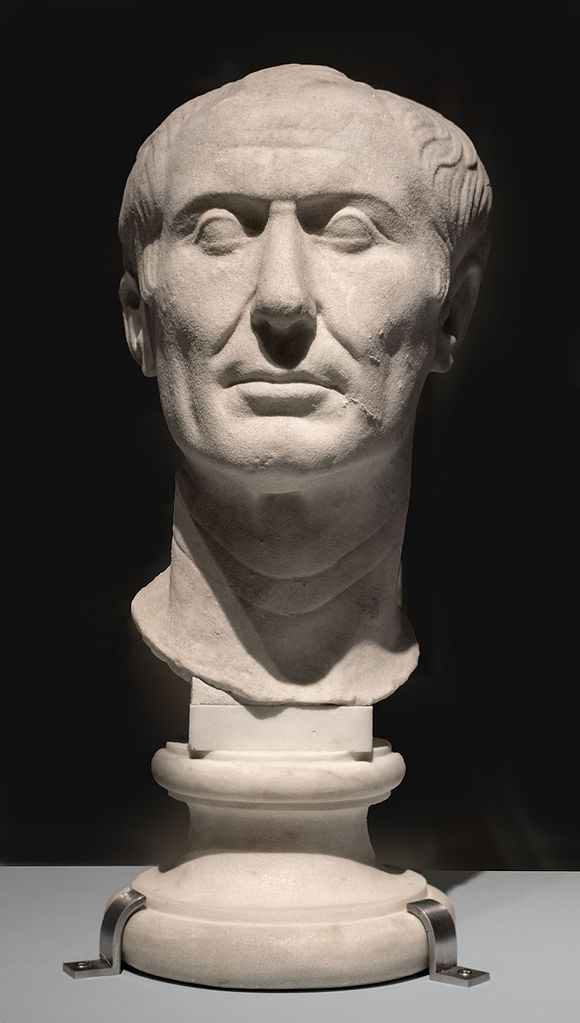
\includegraphics[width=0.5\textwidth]{figures/ceasar.jpg}\\
				\hspace*{15pt}\hbox{\scriptsize Image By:\thinspace{\itshape Ángel M. Felicísimo}}
				%https://commons.wikimedia.org/wiki/File:Retrato_de_Julio_C%C3%A9sar_(26724093101).jpg
			\end{center}

			\column{0.455\textwidth}
			\begin{center}
				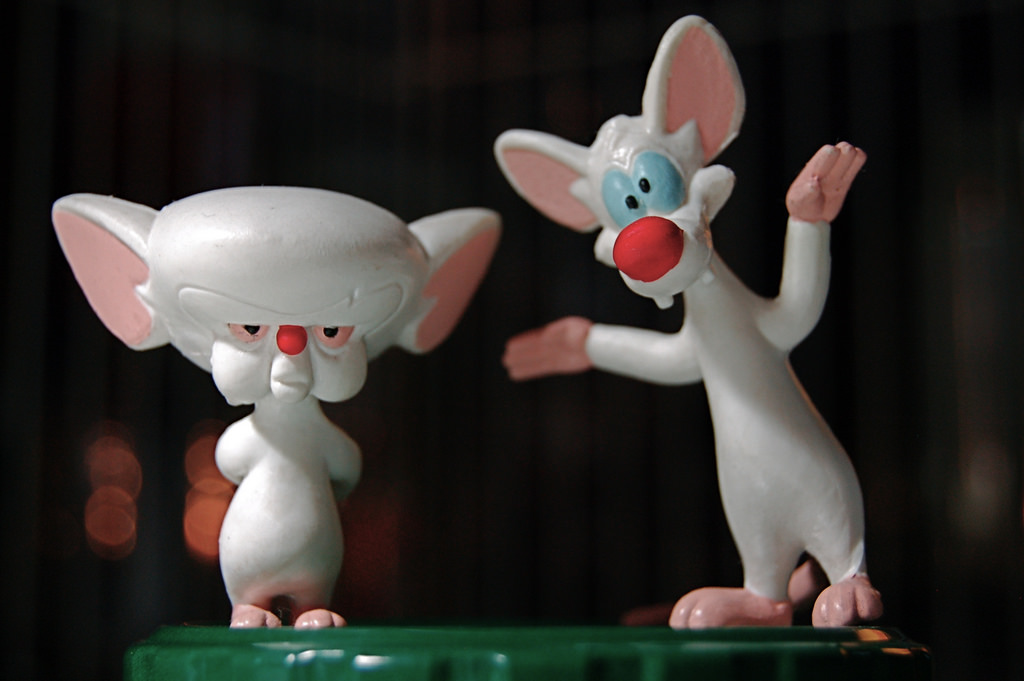
\includegraphics[width=0.9\textwidth]{figures/pinky.jpg}\\
				\hspace*{15pt}\hbox{\scriptsize Image By:\thinspace{\itshape JD Hancock}}
				%https://commons.wikimedia.org/wiki/File:Retrato_de_Julio_C%C3%A9sar_(26724093101).jpg

			\end{center}
		\end{columns}
\end{frame}

\begin{frame}
	\frametitle{Ideas for an algorithm}

	\begin{overlayarea}{\textwidth}{\textheight}
		\input{figures/tikz/closestpair_fixed.tex}
		
		\pause
		\begin{exampleblock}{Algorithm}
			\begin{itemize}
				\item \alert<2>{Divide}: Draw vertical line $L$ that has roughly half of the points on each side.
					\pause
				\item \alert<3>{Conquer}: Find the closest pair on each side.
					\pause
				\item \alert<4>{Combine}: Find the closest pair with one point on each side.
					\pause
				\item Return the minimum of these 3.
			\end{itemize}
		\end{exampleblock}	
	\end{overlayarea}
\end{frame}

\begin{frame}
	\frametitle{Did we make things better?}
	\begin{questionblock}{What is the run time of combine?}
		How much time to combine the two halves? Remember that we want to improve over $\Theta(n^2)$.
	\end{questionblock}	
\end{frame}

\begin{frame}
	\frametitle{How do we make it better?}
		\input{figures/tikz/closestpair_fixed2.tex}
	Observation:
	\begin{itemize}
		\item If $\delta$ is the minimum of the smallest distances left and right.
			\pause
		\item Then we only need to consider pairs of points within $\delta$ of $L$.
			\pause
		\item So in this example, none at all!
	\end{itemize}
\end{frame}

\begin{frame}
	\frametitle{Worst-case?}
	\begin{overlayarea}{\textwidth}{\textheight}
			\begin{itemize}
				\item But worst-case all points are in this $2\delta$-strip...
					\pause
				\item But if we sort them by $y$-coordinate (which can be done in $O(n\log n)$), then how many comparisons do we need?
					\pause
				\item Still $O(n^2)$!?
					\only<4->{
				\item Nope! We only need to check within 11 (i.e. a constant number of) positions in the sorted list.
				}
					\only<5->{
				\item So the combining step is $O(n \log n)$ (which can be further improved to $O(n)$)!
				}
			\end{itemize}
			\only<3>{
			\begin{center}
				
\includegraphics[width=0.4\textwidth]{figures/dilbert.jpg}
				\framesubtitle{http://thecontextofthings.com/wp-content/uploads/2017/11/dilbert-work.jpg}
			\end{center}
		}
	\end{overlayarea}
\end{frame}

\begin{frame}
	\frametitle{Why 11?}

	\begin{overlayarea}{\textwidth}{\textheight}
		\begin{columns}
			\column{0.655\textwidth}
			\begin{block}{Definition}
				Let $s_i$ be the point in the $2\delta$-strip with the $i^\text{th}$ smallest $y$-coordinate.
			\end{block}	
			
			\pause
			\begin{block}{Claim about 11}
				If $|i-j| > 11$ then the distance between $s_i$ and $s_j$ is at least $\delta$.
			\end{block}
			\column{0.255\textwidth}
			\input{figures/tikz/closestpair_delta.tex}	
		\end{columns}
		
		\pause
		\only<3-5>{
			\begin{block}{Proof sketch}
			\begin{itemize}
				\item No two points are in the same $0.5\delta$-by-$0.5\delta$-box.
					\only<4->{
				\item Two points that have two rows between them have a distance $\geq 2\cdot(0.5\delta) = \delta$.
				}
				\only<5->{
				\item So we only consider points at most 2 rows away.
				}
			\end{itemize}
		\end{block}
	}
	\only<6->{
		\begin{exampleblock}{Fun facts!}
			\begin{itemize}
				\item We can even reduce this to just 7 points.
					\only<7>{
				\item Even less if we consider columns separately.
				}
			\end{itemize}
		\end{exampleblock}	
	}
		
		\only<3>{
		\begin{questionblock}{Why not?}
			Why are there no two points in the same box?
		\end{questionblock}
}
	\end{overlayarea}
\end{frame}

\begin{frame}
	\frametitle{The algorithm}
	\begin{columns}
		\column{0.705\textwidth}
	\begin{algorithmic}
		\State Sort all points by x-coordinate
		\Function{Closest-Pair}{$p_1,\dots,p_n$}
			\If{n=1}
				\State \Return $\infty$
			\EndIf

			\pause
			\State $L \gets$ \alert<2>{median} $x$-coordinate
			\State $\delta_1 \gets$ \Call{Closest-Pair}{Points left of $L$}
			\State $\delta_2 \gets$ \Call{Closest-Pair}{Points right of $L$}
			\State $\delta \gets \min(\delta_1,\delta_2)$
			\pause
			\State get list of all points within $\delta$ from L.
			\State sort this list by y-coordinate
			\pause
			\State Scan by y-order, compare every point to the next 11 and update $\delta$ as you go.
			\State \Return $\delta$
		\EndFunction
	\end{algorithmic}
		\pnote{Why not the average?}
		\column{0.205\textwidth}
		\pause
		\begin{questionblock}{}
			What is the recurrence equation for the run time?	
		\end{questionblock}	
		\pause
		\begin{answerblock}{}
			\small
			$T(n) =2T(n/2) + O(n\log n)$	
		\end{answerblock}
	\end{columns}
	
\end{frame}

	\pnote{Why is this relevant? Answers: For instance collision detection algorithms}
\end{frame}

\begin{frame}
	\frametitle{Let's just brute-force it?}
	\begin{overlayarea}{\textwidth}{\textheight}
		\section{Closest pair of points}
\label{sec:closest_pair_of_points}


\begin{frame}
	\frametitle{A new problem}
	\begin{problemblock}{Closest pair of points}
		Given a set of points, what is the pair of points that is closest to each other?\\
		\pause
		More formally:
		\begin{itemize}
			\item Given a set of points $S$, where every point $p_i$ has an x-coordinate $x_i$ and y-coordinate $y_i$.
			\item Distance is defined as: $d(i,j) = \sqrt{{(x_i - x_j)}^{2} + {(y_i-y_j)}^2}$
			\item What is the pair of points $i,j$ such that $d(i,j)$ is minimal?
		\end{itemize}
	\end{problemblock}
	\pause
	\input{figures/tikz/closestpair.tex}
	\pnote{Why is this relevant? Answers: For instance collision detection algorithms}
\end{frame}

\begin{frame}
	\frametitle{Let's just brute-force it?}
	\begin{overlayarea}{\textwidth}{\textheight}
		\input{figures/tikz/closestpair.tex}
		\begin{questionblock}{Brute-force}
			What is the tightest upper bound on the run time for a brute-force solution given $|S| = n$?
			\only<2>{
			\begin{enumerate}[A.]
				\item $O(n \log n)$
				\item $O(n^2)$
				\item $O(n^2 \log n)$
				\item $O(n^3)$
				\item I don't know.
			\end{enumerate}
		}
		\end{questionblock}
		\only<3>{
			\begin{answerblock}{Try every combination}
				We check every pair of points, of which there are $n^2$, so $O(n^2)$.	
			\end{answerblock}
		}
	\end{overlayarea}
\end{frame}

\begin{frame}
	\frametitle{Time to improve!}
	\framesubtitle{Using Divide \& Conquer}
		\begin{columns}
			\column{0.455\textwidth}
			\begin{center}
				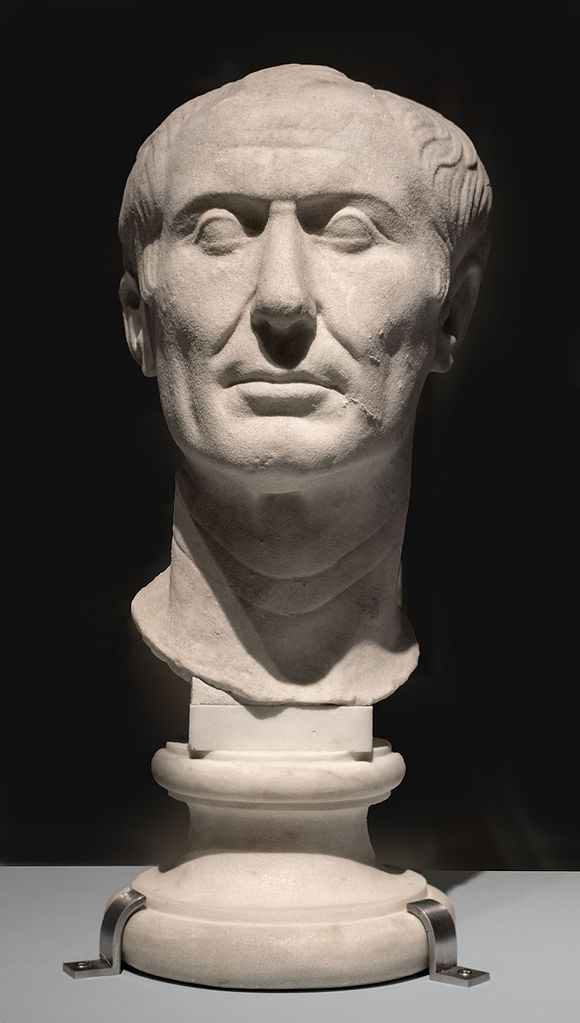
\includegraphics[width=0.5\textwidth]{figures/ceasar.jpg}\\
				\hspace*{15pt}\hbox{\scriptsize Image By:\thinspace{\itshape Ángel M. Felicísimo}}
				%https://commons.wikimedia.org/wiki/File:Retrato_de_Julio_C%C3%A9sar_(26724093101).jpg
			\end{center}

			\column{0.455\textwidth}
			\begin{center}
				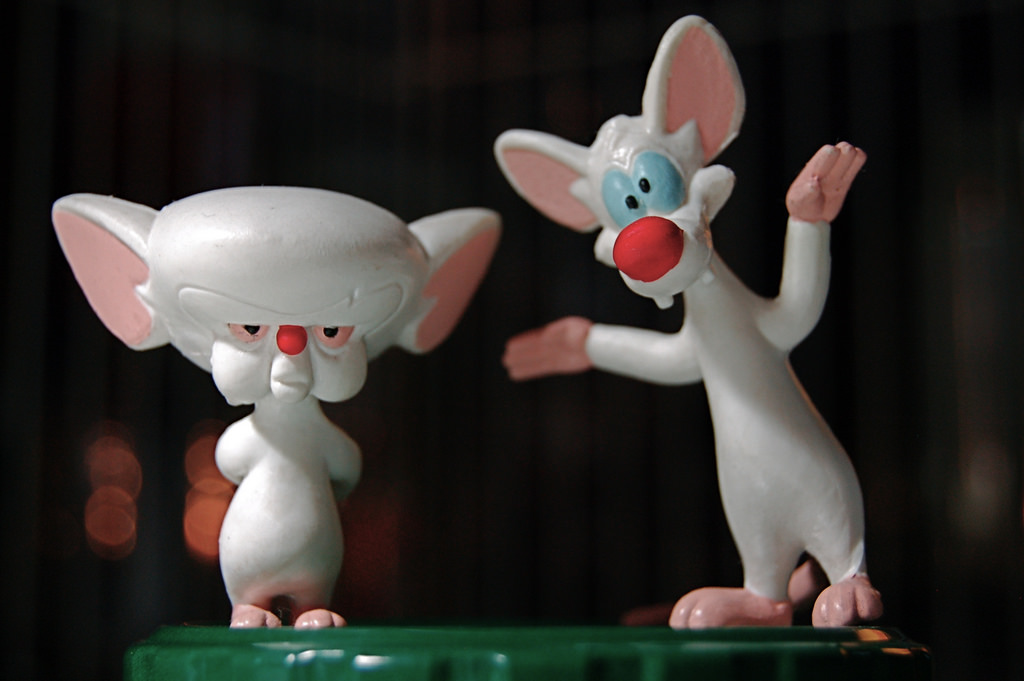
\includegraphics[width=0.9\textwidth]{figures/pinky.jpg}\\
				\hspace*{15pt}\hbox{\scriptsize Image By:\thinspace{\itshape JD Hancock}}
				%https://commons.wikimedia.org/wiki/File:Retrato_de_Julio_C%C3%A9sar_(26724093101).jpg

			\end{center}
		\end{columns}
\end{frame}

\begin{frame}
	\frametitle{Ideas for an algorithm}

	\begin{overlayarea}{\textwidth}{\textheight}
		\input{figures/tikz/closestpair_fixed.tex}
		
		\pause
		\begin{exampleblock}{Algorithm}
			\begin{itemize}
				\item \alert<2>{Divide}: Draw vertical line $L$ that has roughly half of the points on each side.
					\pause
				\item \alert<3>{Conquer}: Find the closest pair on each side.
					\pause
				\item \alert<4>{Combine}: Find the closest pair with one point on each side.
					\pause
				\item Return the minimum of these 3.
			\end{itemize}
		\end{exampleblock}	
	\end{overlayarea}
\end{frame}

\begin{frame}
	\frametitle{Did we make things better?}
	\begin{questionblock}{What is the run time of combine?}
		How much time to combine the two halves? Remember that we want to improve over $\Theta(n^2)$.
	\end{questionblock}	
\end{frame}

\begin{frame}
	\frametitle{How do we make it better?}
		\input{figures/tikz/closestpair_fixed2.tex}
	Observation:
	\begin{itemize}
		\item If $\delta$ is the minimum of the smallest distances left and right.
			\pause
		\item Then we only need to consider pairs of points within $\delta$ of $L$.
			\pause
		\item So in this example, none at all!
	\end{itemize}
\end{frame}

\begin{frame}
	\frametitle{Worst-case?}
	\begin{overlayarea}{\textwidth}{\textheight}
			\begin{itemize}
				\item But worst-case all points are in this $2\delta$-strip...
					\pause
				\item But if we sort them by $y$-coordinate (which can be done in $O(n\log n)$), then how many comparisons do we need?
					\pause
				\item Still $O(n^2)$!?
					\only<4->{
				\item Nope! We only need to check within 11 (i.e. a constant number of) positions in the sorted list.
				}
					\only<5->{
				\item So the combining step is $O(n \log n)$ (which can be further improved to $O(n)$)!
				}
			\end{itemize}
			\only<3>{
			\begin{center}
				
\includegraphics[width=0.4\textwidth]{figures/dilbert.jpg}
				\framesubtitle{http://thecontextofthings.com/wp-content/uploads/2017/11/dilbert-work.jpg}
			\end{center}
		}
	\end{overlayarea}
\end{frame}

\begin{frame}
	\frametitle{Why 11?}

	\begin{overlayarea}{\textwidth}{\textheight}
		\begin{columns}
			\column{0.655\textwidth}
			\begin{block}{Definition}
				Let $s_i$ be the point in the $2\delta$-strip with the $i^\text{th}$ smallest $y$-coordinate.
			\end{block}	
			
			\pause
			\begin{block}{Claim about 11}
				If $|i-j| > 11$ then the distance between $s_i$ and $s_j$ is at least $\delta$.
			\end{block}
			\column{0.255\textwidth}
			\input{figures/tikz/closestpair_delta.tex}	
		\end{columns}
		
		\pause
		\only<3-5>{
			\begin{block}{Proof sketch}
			\begin{itemize}
				\item No two points are in the same $0.5\delta$-by-$0.5\delta$-box.
					\only<4->{
				\item Two points that have two rows between them have a distance $\geq 2\cdot(0.5\delta) = \delta$.
				}
				\only<5->{
				\item So we only consider points at most 2 rows away.
				}
			\end{itemize}
		\end{block}
	}
	\only<6->{
		\begin{exampleblock}{Fun facts!}
			\begin{itemize}
				\item We can even reduce this to just 7 points.
					\only<7>{
				\item Even less if we consider columns separately.
				}
			\end{itemize}
		\end{exampleblock}	
	}
		
		\only<3>{
		\begin{questionblock}{Why not?}
			Why are there no two points in the same box?
		\end{questionblock}
}
	\end{overlayarea}
\end{frame}

\begin{frame}
	\frametitle{The algorithm}
	\begin{columns}
		\column{0.705\textwidth}
	\begin{algorithmic}
		\State Sort all points by x-coordinate
		\Function{Closest-Pair}{$p_1,\dots,p_n$}
			\If{n=1}
				\State \Return $\infty$
			\EndIf

			\pause
			\State $L \gets$ \alert<2>{median} $x$-coordinate
			\State $\delta_1 \gets$ \Call{Closest-Pair}{Points left of $L$}
			\State $\delta_2 \gets$ \Call{Closest-Pair}{Points right of $L$}
			\State $\delta \gets \min(\delta_1,\delta_2)$
			\pause
			\State get list of all points within $\delta$ from L.
			\State sort this list by y-coordinate
			\pause
			\State Scan by y-order, compare every point to the next 11 and update $\delta$ as you go.
			\State \Return $\delta$
		\EndFunction
	\end{algorithmic}
		\pnote{Why not the average?}
		\column{0.205\textwidth}
		\pause
		\begin{questionblock}{}
			What is the recurrence equation for the run time?	
		\end{questionblock}	
		\pause
		\begin{answerblock}{}
			\small
			$T(n) =2T(n/2) + O(n\log n)$	
		\end{answerblock}
	\end{columns}
	
\end{frame}

		\begin{questionblock}{Brute-force}
			What is the tightest upper bound on the run time for a brute-force solution given $|S| = n$?
			\only<2>{
			\begin{enumerate}[A.]
				\item $O(n \log n)$
				\item $O(n^2)$
				\item $O(n^2 \log n)$
				\item $O(n^3)$
				\item I don't know.
			\end{enumerate}
		}
		\end{questionblock}
		\only<3>{
			\begin{answerblock}{Try every combination}
				We check every pair of points, of which there are $n^2$, so $O(n^2)$.	
			\end{answerblock}
		}
	\end{overlayarea}
\end{frame}

\begin{frame}
	\frametitle{Time to improve!}
	\framesubtitle{Using Divide \& Conquer}
		\begin{columns}
			\column{0.455\textwidth}
			\begin{center}
				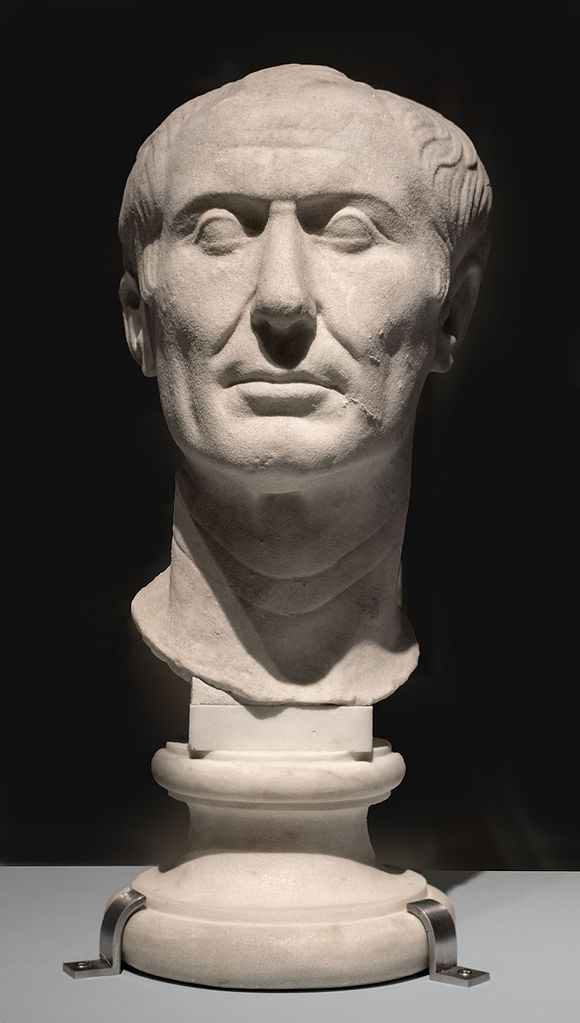
\includegraphics[width=0.5\textwidth]{figures/ceasar.jpg}\\
				\hspace*{15pt}\hbox{\scriptsize Image By:\thinspace{\itshape Ángel M. Felicísimo}}
				%https://commons.wikimedia.org/wiki/File:Retrato_de_Julio_C%C3%A9sar_(26724093101).jpg
			\end{center}

			\column{0.455\textwidth}
			\begin{center}
				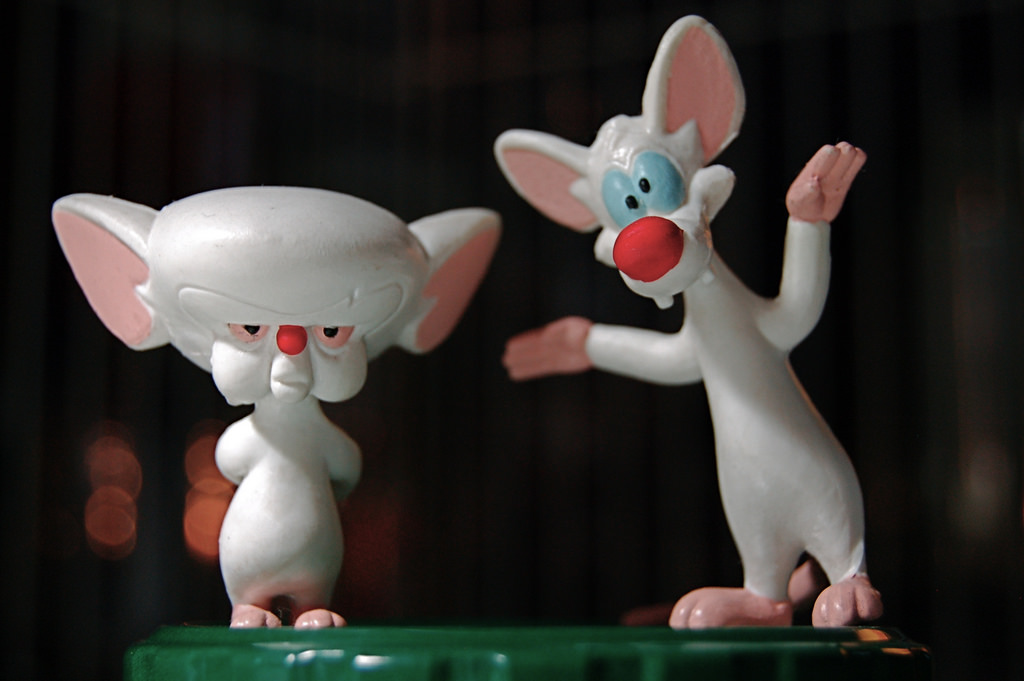
\includegraphics[width=0.9\textwidth]{figures/pinky.jpg}\\
				\hspace*{15pt}\hbox{\scriptsize Image By:\thinspace{\itshape JD Hancock}}
				%https://commons.wikimedia.org/wiki/File:Retrato_de_Julio_C%C3%A9sar_(26724093101).jpg

			\end{center}
		\end{columns}
\end{frame}

\begin{frame}
	\frametitle{Ideas for an algorithm}

	\begin{overlayarea}{\textwidth}{\textheight}
		\begin{figure}[htpb]
\begin{center}
\begin{tikzpicture}[scale=0.5, transform shape]
	\draw (-8,-3) rectangle (8,3);

	\foreach \x/\y/\name in {
		-7/2/,
		-6/1/l1,
		-5/1/l2,
		-3/-2/c1,
		-1/-2/c2,
		3/-1/,
		5/1.5/r1,
		5/0/r2,
		}{
		\node[circle, black, draw, fill=blue!30, minimum size=4pt] (\name) at (\x,\y) {};
	}
		\node at (-1.5, -3.5) {};
	\only<2->{
		\draw[dotted] (-1.5,-3) -- (-1.5,3);
		\node at (-1.5, -3.5) {\Large $L$};
	}
	\only<3->{
		\draw[dotted, red, thick] (l1) --  node[anchor=south] {\Large 1} (l2);
		\draw[dotted, red, thick] (r1) --  node[anchor=west] {\Large 1.5} (r2);
	}
	\only<4->{
		\draw[dotted, red, thick] (c1) --  node[anchor=south] {\Large 2} (c2);
	}
\end{tikzpicture}
\end{center}
\end{figure}

		
		\pause
		\begin{exampleblock}{Algorithm}
			\begin{itemize}
				\item \alert<2>{Divide}: Draw vertical line $L$ that has roughly half of the points on each side.
					\pause
				\item \alert<3>{Conquer}: Find the closest pair on each side.
					\pause
				\item \alert<4>{Combine}: Find the closest pair with one point on each side.
					\pause
				\item Return the minimum of these 3.
			\end{itemize}
		\end{exampleblock}	
	\end{overlayarea}
\end{frame}

\begin{frame}
	\frametitle{Did we make things better?}
	\begin{questionblock}{What is the run time of combine?}
		How much time to combine the two halves? Remember that we want to improve over $\Theta(n^2)$.
	\end{questionblock}	
\end{frame}

\begin{frame}
	\frametitle{How do we make it better?}
		\begin{figure}[htpb]
\begin{center}
\begin{tikzpicture}[scale=0.5, transform shape]
	\draw (-8,-3) rectangle (8,3);

	\only<2->{
		\draw[fill=gray!10] (-2.5,-3) rectangle (-0.5,3);
	}
	\foreach \x/\y/\name in {
		-7/2/,
		-6/1/l1,
		-5/1/l2,
		-3/-2/c1,
		-1/-2/c2,
		3/-1/,
		5/1.5/r1,
		5/0/r2,
		}{
		\node[circle, black, draw, fill=blue!30, minimum size=4pt] (\name) at (\x,\y) {};
	}
		\draw[dotted] (-1.5,-3) -- (-1.5,3);
		\node at (-1.5, -3.5) {\Large $L$};
		\draw[dotted, red, thick] (l1) --  node[anchor=south] {\Large 1} (l2);
		\draw[dotted, red, thick] (r1) --  node[anchor=west] {\Large 1.5} (r2);
		\draw[dotted, red, thick] (c1) --  node[anchor=south] {\Large 2} (c2);

\end{tikzpicture}
\end{center}
\end{figure}

	Observation:
	\begin{itemize}
		\item If $\delta$ is the minimum of the smallest distances left and right.
			\pause
		\item Then we only need to consider pairs of points within $\delta$ of $L$.
			\pause
		\item So in this example, none at all!
	\end{itemize}
\end{frame}

\begin{frame}
	\frametitle{Worst-case?}
	\begin{overlayarea}{\textwidth}{\textheight}
			\begin{itemize}
				\item But worst-case all points are in this $2\delta$-strip...
					\pause
				\item But if we sort them by $y$-coordinate (which can be done in $O(n\log n)$), then how many comparisons do we need?
					\pause
				\item Still $O(n^2)$!?
					\only<4->{
				\item Nope! We only need to check within 11 (i.e. a constant number of) positions in the sorted list.
				}
					\only<5->{
				\item So the combining step is $O(n \log n)$ (which can be further improved to $O(n)$)!
				}
			\end{itemize}
			\only<3>{
			\begin{center}
				
\includegraphics[width=0.4\textwidth]{figures/dilbert.jpg}
				\framesubtitle{http://thecontextofthings.com/wp-content/uploads/2017/11/dilbert-work.jpg}
			\end{center}
		}
	\end{overlayarea}
\end{frame}

\begin{frame}
	\frametitle{Why 11?}

	\begin{overlayarea}{\textwidth}{\textheight}
		\begin{columns}
			\column{0.655\textwidth}
			\begin{block}{Definition}
				Let $s_i$ be the point in the $2\delta$-strip with the $i^\text{th}$ smallest $y$-coordinate.
			\end{block}	
			
			\pause
			\begin{block}{Claim about 11}
				If $|i-j| > 11$ then the distance between $s_i$ and $s_j$ is at least $\delta$.
			\end{block}
			\column{0.255\textwidth}
			\begin{figure}[htpb]
\begin{center}
\begin{tikzpicture}[scale=0.4, transform shape]
	\draw (-2,-4) rectangle (2,4);
	
	\only<5->{
		\foreach \y in {-2, ..., 0}{
			\foreach \x in {-2, ..., 1}{
				\draw[fill=green!30] (\x,\y) rectangle (\x+1,\y+1);
			}
		}
	}

	\foreach \x/\y/\name/\color in {
		1.35/-2.4/1/red,
		-1.35/-1.6/2/green,
		-0.4/-0.4/3/blue,
		1.3/0.5/4/blue,
	%	1.7/1.4/5/red,
		-0.4/2.4/5/red,
		0.3/2.4/6/red}{
		\alt<4->{
		\node[circle, black, draw, fill=\color!30, minimum size=4pt] () at (\x,\y) {\name};
			}{
		\node[circle, black, draw, fill=blue!30, minimum size=4pt] () at (\x,\y) {\name};
		}
	}
		\draw[thick] (0,-4) -- (0,4);
		\node at (0, -4.5) {\Large $L$};
		\node at (-2, -4.5) {\Large $L-\delta$};
		\node at (2, -4.5) {\Large $L+\delta$};
		\only<3->{
			\draw[dotted] (1,-4) -- (1,4);
			\draw[dotted] (-1,-4) -- (-1,4);

			\foreach \y in {-3, ..., 3}{
				\draw[dotted] (-2,\y) -- (2,\y);
			}
		}

\end{tikzpicture}
\end{center}
\end{figure}
	
		\end{columns}
		
		\pause
		\only<3-5>{
			\begin{block}{Proof sketch}
			\begin{itemize}
				\item No two points are in the same $0.5\delta$-by-$0.5\delta$-box.
					\only<4->{
				\item Two points that have two rows between them have a distance $\geq 2\cdot(0.5\delta) = \delta$.
				}
				\only<5->{
				\item So we only consider points at most 2 rows away.
				}
			\end{itemize}
		\end{block}
	}
	\only<6->{
		\begin{exampleblock}{Fun facts!}
			\begin{itemize}
				\item We can even reduce this to just 7 points.
					\only<7>{
				\item Even less if we consider columns separately.
				}
			\end{itemize}
		\end{exampleblock}	
	}
		
		\only<3>{
		\begin{questionblock}{Why not?}
			Why are there no two points in the same box?
		\end{questionblock}
}
	\end{overlayarea}
\end{frame}

\begin{frame}
	\frametitle{The algorithm}
	\begin{columns}
		\column{0.705\textwidth}
	\begin{algorithmic}
		\State Sort all points by x-coordinate
		\Function{Closest-Pair}{$p_1,\dots,p_n$}
			\If{n=1}
				\State \Return $\infty$
			\EndIf

			\pause
			\State $L \gets$ \alert<2>{median} $x$-coordinate
			\State $\delta_1 \gets$ \Call{Closest-Pair}{Points left of $L$}
			\State $\delta_2 \gets$ \Call{Closest-Pair}{Points right of $L$}
			\State $\delta \gets \min(\delta_1,\delta_2)$
			\pause
			\State get list of all points within $\delta$ from L.
			\State sort this list by y-coordinate
			\pause
			\State Scan by y-order, compare every point to the next 11 and update $\delta$ as you go.
			\State \Return $\delta$
		\EndFunction
	\end{algorithmic}
		\pnote{Why not the average?}
		\column{0.205\textwidth}
		\pause
		\begin{questionblock}{}
			What is the recurrence equation for the run time?	
		\end{questionblock}	
		\pause
		\begin{answerblock}{}
			\small
			$T(n) =2T(n/2) + O(n\log n)$	
		\end{answerblock}
	\end{columns}
	
\end{frame}

		\begin{questionblock}{Brute-force}
			What is the tightest upper bound on the run time for a brute-force solution given $|S| = n$?
			\only<2>{
			\begin{enumerate}[A.]
				\item $O(n \log n)$
				\item $O(n^2)$
				\item $O(n^2 \log n)$
				\item $O(n^3)$
				\item I don't know.
			\end{enumerate}
		}
		\end{questionblock}
		\only<3>{
			\begin{answerblock}{Try every combination}
				We check every pair of points, of which there are $n^2$, so $O(n^2)$.	
			\end{answerblock}
		}
	\end{overlayarea}
\end{frame}

\begin{frame}
	\frametitle{Time to improve!}
	\framesubtitle{Using Divide \& Conquer}
		\begin{columns}
			\column{0.455\textwidth}
			\begin{center}
				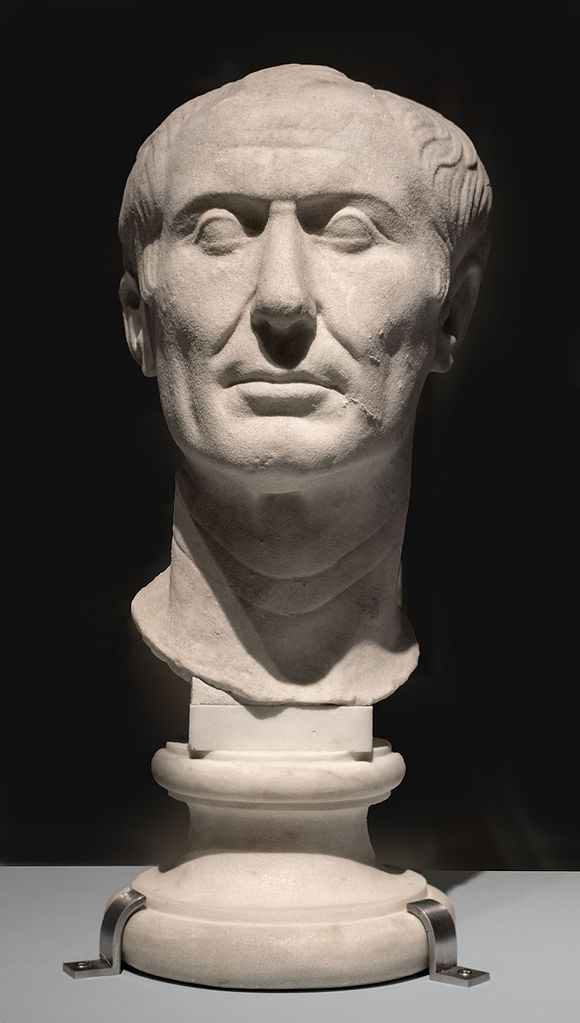
\includegraphics[width=0.5\textwidth]{figures/ceasar.jpg}\\
				\hspace*{15pt}\hbox{\scriptsize Image By:\thinspace{\itshape Ángel M. Felicísimo}}
				%https://commons.wikimedia.org/wiki/File:Retrato_de_Julio_C%C3%A9sar_(26724093101).jpg
			\end{center}

			\column{0.455\textwidth}
			\begin{center}
				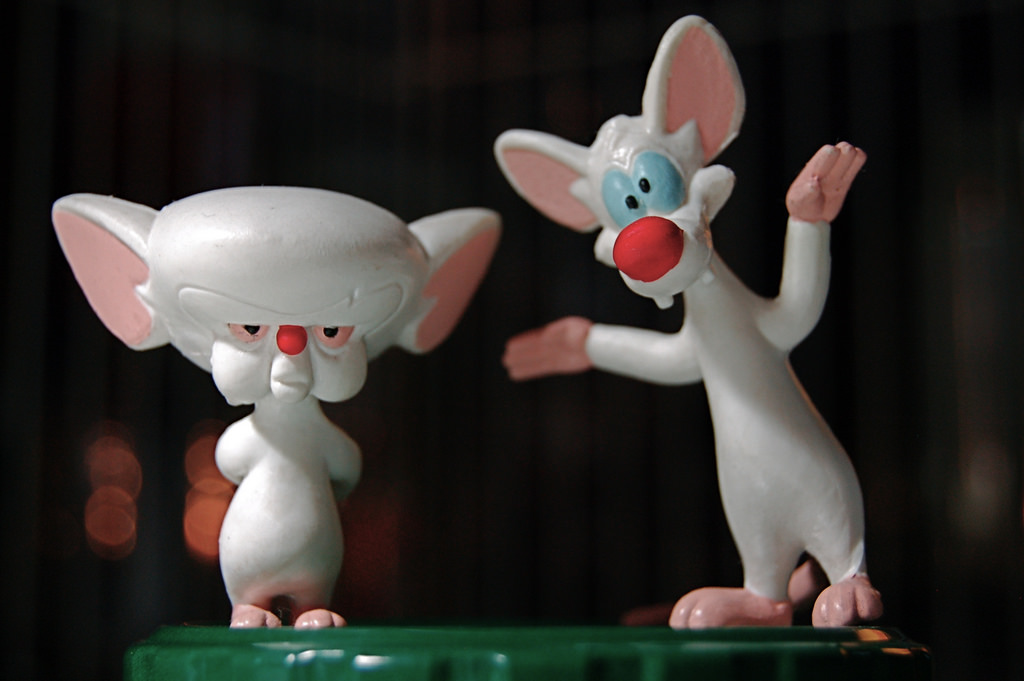
\includegraphics[width=0.9\textwidth]{figures/pinky.jpg}\\
				\hspace*{15pt}\hbox{\scriptsize Image By:\thinspace{\itshape JD Hancock}}
				%https://commons.wikimedia.org/wiki/File:Retrato_de_Julio_C%C3%A9sar_(26724093101).jpg

			\end{center}
		\end{columns}
\end{frame}

\begin{frame}
	\frametitle{Ideas for an algorithm}

	\begin{overlayarea}{\textwidth}{\textheight}
		\begin{figure}[htpb]
\begin{center}
\begin{tikzpicture}[scale=0.5, transform shape]
	\draw (-8,-3) rectangle (8,3);

	\foreach \x/\y/\name in {
		-7/2/,
		-6/1/l1,
		-5/1/l2,
		-3/-2/c1,
		-1/-2/c2,
		3/-1/,
		5/1.5/r1,
		5/0/r2,
		}{
		\node[circle, black, draw, fill=blue!30, minimum size=4pt] (\name) at (\x,\y) {};
	}
		\node at (-1.5, -3.5) {};
	\only<2->{
		\draw[dotted] (-1.5,-3) -- (-1.5,3);
		\node at (-1.5, -3.5) {\Large $L$};
	}
	\only<3->{
		\draw[dotted, red, thick] (l1) --  node[anchor=south] {\Large 1} (l2);
		\draw[dotted, red, thick] (r1) --  node[anchor=west] {\Large 1.5} (r2);
	}
	\only<4->{
		\draw[dotted, red, thick] (c1) --  node[anchor=south] {\Large 2} (c2);
	}
\end{tikzpicture}
\end{center}
\end{figure}

		
		\pause
		\begin{exampleblock}{Algorithm}
			\begin{itemize}
				\item \alert<2>{Divide}: Draw vertical line $L$ that has roughly half of the points on each side.
					\pause
				\item \alert<3>{Conquer}: Find the closest pair on each side.
					\pause
				\item \alert<4>{Combine}: Find the closest pair with one point on each side.
					\pause
				\item Return the minimum of these 3.
			\end{itemize}
		\end{exampleblock}	
	\end{overlayarea}
\end{frame}

\begin{frame}
	\frametitle{Did we make things better?}
	\begin{questionblock}{What is the run time of combine?}
		How much time to combine the two halves? Remember that we want to improve over $\Theta(n^2)$.
	\end{questionblock}	
\end{frame}

\begin{frame}
	\frametitle{How do we make it better?}
		\begin{figure}[htpb]
\begin{center}
\begin{tikzpicture}[scale=0.5, transform shape]
	\draw (-8,-3) rectangle (8,3);

	\only<2->{
		\draw[fill=gray!10] (-2.5,-3) rectangle (-0.5,3);
	}
	\foreach \x/\y/\name in {
		-7/2/,
		-6/1/l1,
		-5/1/l2,
		-3/-2/c1,
		-1/-2/c2,
		3/-1/,
		5/1.5/r1,
		5/0/r2,
		}{
		\node[circle, black, draw, fill=blue!30, minimum size=4pt] (\name) at (\x,\y) {};
	}
		\draw[dotted] (-1.5,-3) -- (-1.5,3);
		\node at (-1.5, -3.5) {\Large $L$};
		\draw[dotted, red, thick] (l1) --  node[anchor=south] {\Large 1} (l2);
		\draw[dotted, red, thick] (r1) --  node[anchor=west] {\Large 1.5} (r2);
		\draw[dotted, red, thick] (c1) --  node[anchor=south] {\Large 2} (c2);

\end{tikzpicture}
\end{center}
\end{figure}

	Observation:
	\begin{itemize}
		\item If $\delta$ is the minimum of the smallest distances left and right.
			\pause
		\item Then we only need to consider pairs of points within $\delta$ of $L$.
			\pause
		\item So in this example, none at all!
	\end{itemize}
\end{frame}

\begin{frame}
	\frametitle{Worst-case?}
	\begin{overlayarea}{\textwidth}{\textheight}
			\begin{itemize}
				\item But worst-case all points are in this $2\delta$-strip...
					\pause
				\item But if we sort them by $y$-coordinate (which can be done in $O(n\log n)$), then how many comparisons do we need?
					\pause
				\item Still $O(n^2)$!?
					\only<4->{
				\item Nope! We only need to check within 11 (i.e. a constant number of) positions in the sorted list.
				}
					\only<5->{
				\item So the combining step is $O(n \log n)$ (which can be further improved to $O(n)$)!
				}
			\end{itemize}
			\only<3>{
			\begin{center}
				
\includegraphics[width=0.4\textwidth]{figures/dilbert.jpg}
				\framesubtitle{http://thecontextofthings.com/wp-content/uploads/2017/11/dilbert-work.jpg}
			\end{center}
		}
	\end{overlayarea}
\end{frame}

\begin{frame}
	\frametitle{Why 11?}

	\begin{overlayarea}{\textwidth}{\textheight}
		\begin{columns}
			\column{0.655\textwidth}
			\begin{block}{Definition}
				Let $s_i$ be the point in the $2\delta$-strip with the $i^\text{th}$ smallest $y$-coordinate.
			\end{block}	
			
			\pause
			\begin{block}{Claim about 11}
				If $|i-j| > 11$ then the distance between $s_i$ and $s_j$ is at least $\delta$.
			\end{block}
			\column{0.255\textwidth}
			\begin{figure}[htpb]
\begin{center}
\begin{tikzpicture}[scale=0.4, transform shape]
	\draw (-2,-4) rectangle (2,4);
	
	\only<5->{
		\foreach \y in {-2, ..., 0}{
			\foreach \x in {-2, ..., 1}{
				\draw[fill=green!30] (\x,\y) rectangle (\x+1,\y+1);
			}
		}
	}

	\foreach \x/\y/\name/\color in {
		1.35/-2.4/1/red,
		-1.35/-1.6/2/green,
		-0.4/-0.4/3/blue,
		1.3/0.5/4/blue,
	%	1.7/1.4/5/red,
		-0.4/2.4/5/red,
		0.3/2.4/6/red}{
		\alt<4->{
		\node[circle, black, draw, fill=\color!30, minimum size=4pt] () at (\x,\y) {\name};
			}{
		\node[circle, black, draw, fill=blue!30, minimum size=4pt] () at (\x,\y) {\name};
		}
	}
		\draw[thick] (0,-4) -- (0,4);
		\node at (0, -4.5) {\Large $L$};
		\node at (-2, -4.5) {\Large $L-\delta$};
		\node at (2, -4.5) {\Large $L+\delta$};
		\only<3->{
			\draw[dotted] (1,-4) -- (1,4);
			\draw[dotted] (-1,-4) -- (-1,4);

			\foreach \y in {-3, ..., 3}{
				\draw[dotted] (-2,\y) -- (2,\y);
			}
		}

\end{tikzpicture}
\end{center}
\end{figure}
	
		\end{columns}
		
		\pause
		\only<3-5>{
			\begin{block}{Proof sketch}
			\begin{itemize}
				\item No two points are in the same $0.5\delta$-by-$0.5\delta$-box.
					\only<4->{
				\item Two points that have two rows between them have a distance $\geq 2\cdot(0.5\delta) = \delta$.
				}
				\only<5->{
				\item So we only consider points at most 2 rows away.
				}
			\end{itemize}
		\end{block}
	}
	\only<6->{
		\begin{exampleblock}{Fun facts!}
			\begin{itemize}
				\item We can even reduce this to just 7 points.
					\only<7>{
				\item Even less if we consider columns separately.
				}
			\end{itemize}
		\end{exampleblock}	
	}
		
		\only<3>{
		\begin{questionblock}{Why not?}
			Why are there no two points in the same box?
		\end{questionblock}
}
	\end{overlayarea}
\end{frame}

\begin{frame}
	\frametitle{The algorithm}
	\begin{columns}
		\column{0.705\textwidth}
	\begin{algorithmic}
		\State Sort all points by x-coordinate
		\Function{Closest-Pair}{$p_1,\dots,p_n$}
			\If{n=1}
				\State \Return $\infty$
			\EndIf

			\pause
			\State $L \gets$ \alert<2>{median} $x$-coordinate
			\State $\delta_1 \gets$ \Call{Closest-Pair}{Points left of $L$}
			\State $\delta_2 \gets$ \Call{Closest-Pair}{Points right of $L$}
			\State $\delta \gets \min(\delta_1,\delta_2)$
			\pause
			\State get list of all points within $\delta$ from L.
			\State sort this list by y-coordinate
			\pause
			\State Scan by y-order, compare every point to the next 11 and update $\delta$ as you go.
			\State \Return $\delta$
		\EndFunction
	\end{algorithmic}
		\pnote{Why not the average?}
		\column{0.205\textwidth}
		\pause
		\begin{questionblock}{}
			What is the recurrence equation for the run time?	
		\end{questionblock}	
		\pause
		\begin{answerblock}{}
			\small
			$T(n) =2T(n/2) + O(n\log n)$	
		\end{answerblock}
	\end{columns}
	
\end{frame}

\section{Intermezzo}
\label{sec:intermezzo}

\begin{frame}
	\frametitle{Intermezzo: Exams}
	\begin{center}
		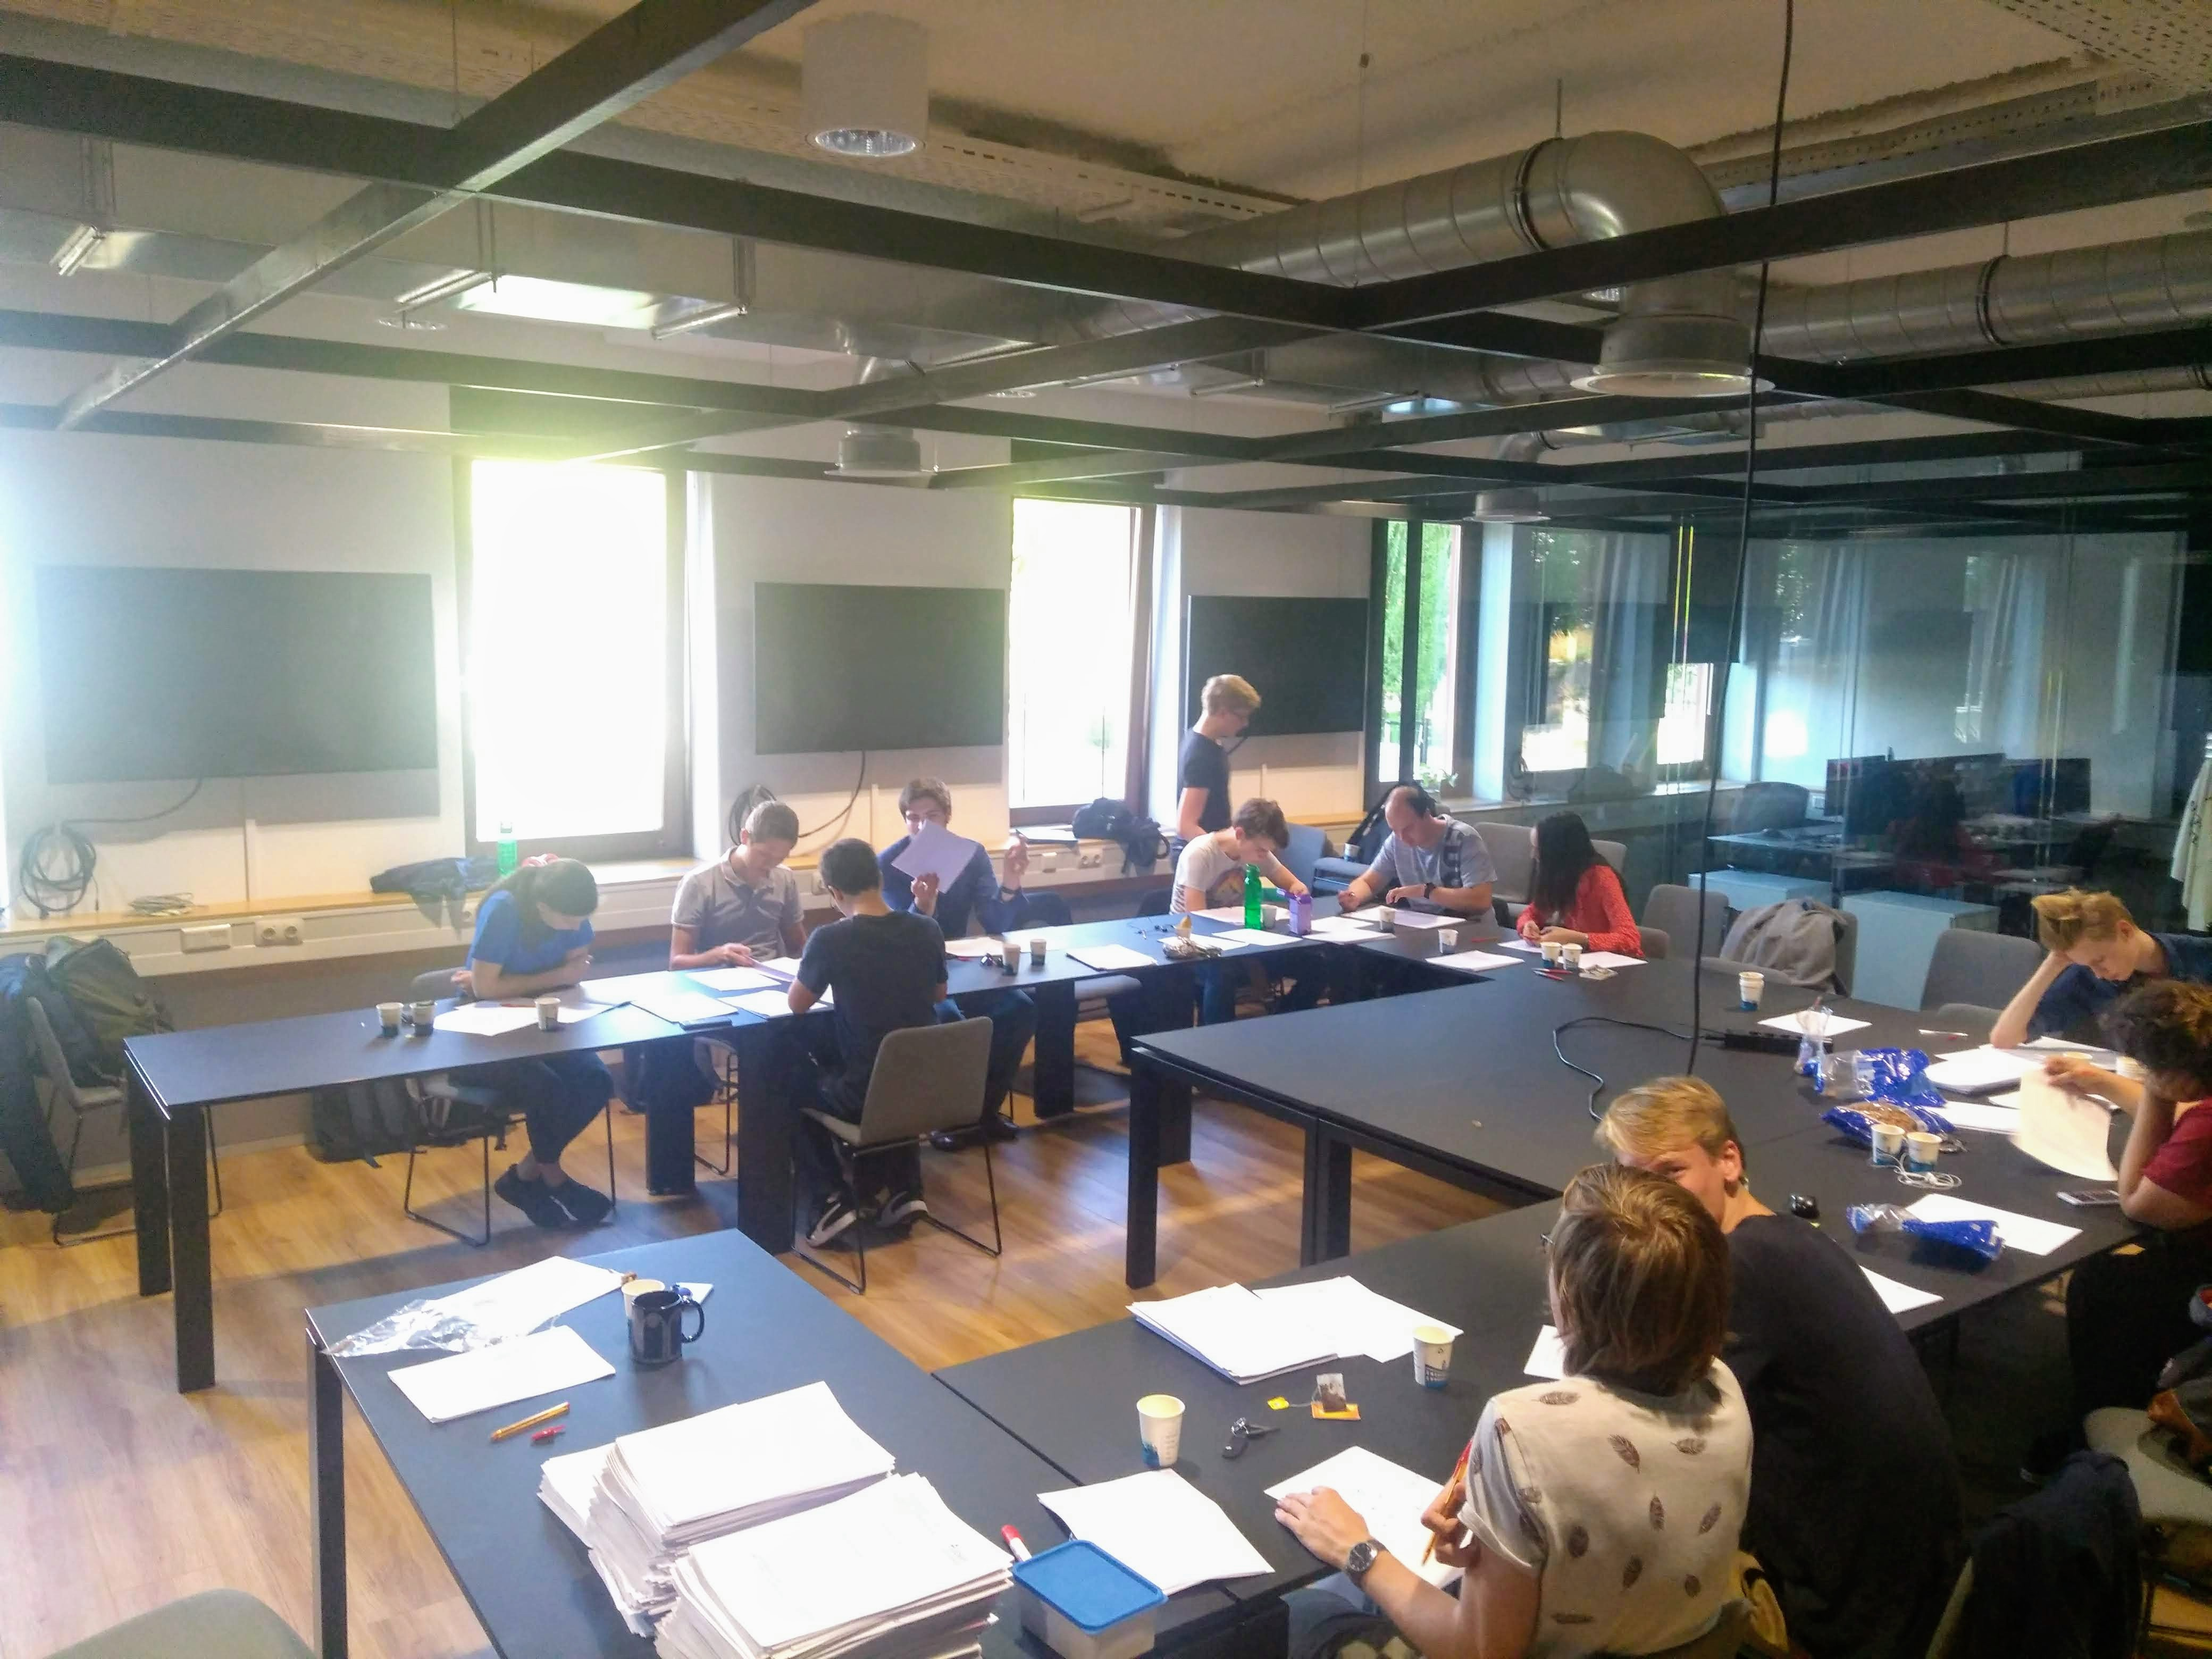
\includegraphics[width=0.6\textwidth]{figures/grading.jpg}\\
		\hspace*{15pt}\hbox{\scriptsize Image By:\thinspace{\itshape Stefan Hugtenburg}}
	\end{center}
\end{frame}

\begin{frame}
	\frametitle{The other type of tree}
	\framesubtitle{\url{https://science.howstuffworks.com/environmental/green-science/question16.htm}}
	\begin{itemize}
		\item We use a lot of paper, when it comes to exams\dots
			\pause
		\item Rough estimate of CSE first year, so far:
			\begin{itemize}
				\item 12 MC forms for 800 people
				\item 8 open question booklets for 800 people (2 sheets of paper each), assume everyone uses only one.
				\item 17 exams for 800 people, lets estimate that at 8 sheets each.
			\end{itemize}
			\pause
		\item	That's roughly 130-thousand sheets of paper.
			\pause
		\item Which is about 1.5 trees, according to howstuffworks.com
	\end{itemize}
\end{frame}

\begin{frame}
	\frametitle{Other interesting tree facts}
	\framesubtitle{\url{https://www.treesaregood.org/funfacts}}
	
	\begin{itemize}
		\item The oldest tree in the world is estimated at being 4765 years old.
			\pause
		\item The study of deteriming the age of a tree is called dendrochronology.
			\pause
		\item You are willing to pay more for goods and services if there are trees nearby! (slightly paraphrased)
			\pause
		\item Want to know more about where trees get their mass? Check this YouTube video:
			\url{https://www.youtu.be/2KZb2_vcNTg}
	\end{itemize}
\end{frame}


\section{The Master Method}
\label{sec:the_master_method}

\begin{frame}
	\frametitle{The master method}
	\framesubtitle{Not in the book!}
	\begin{center}
		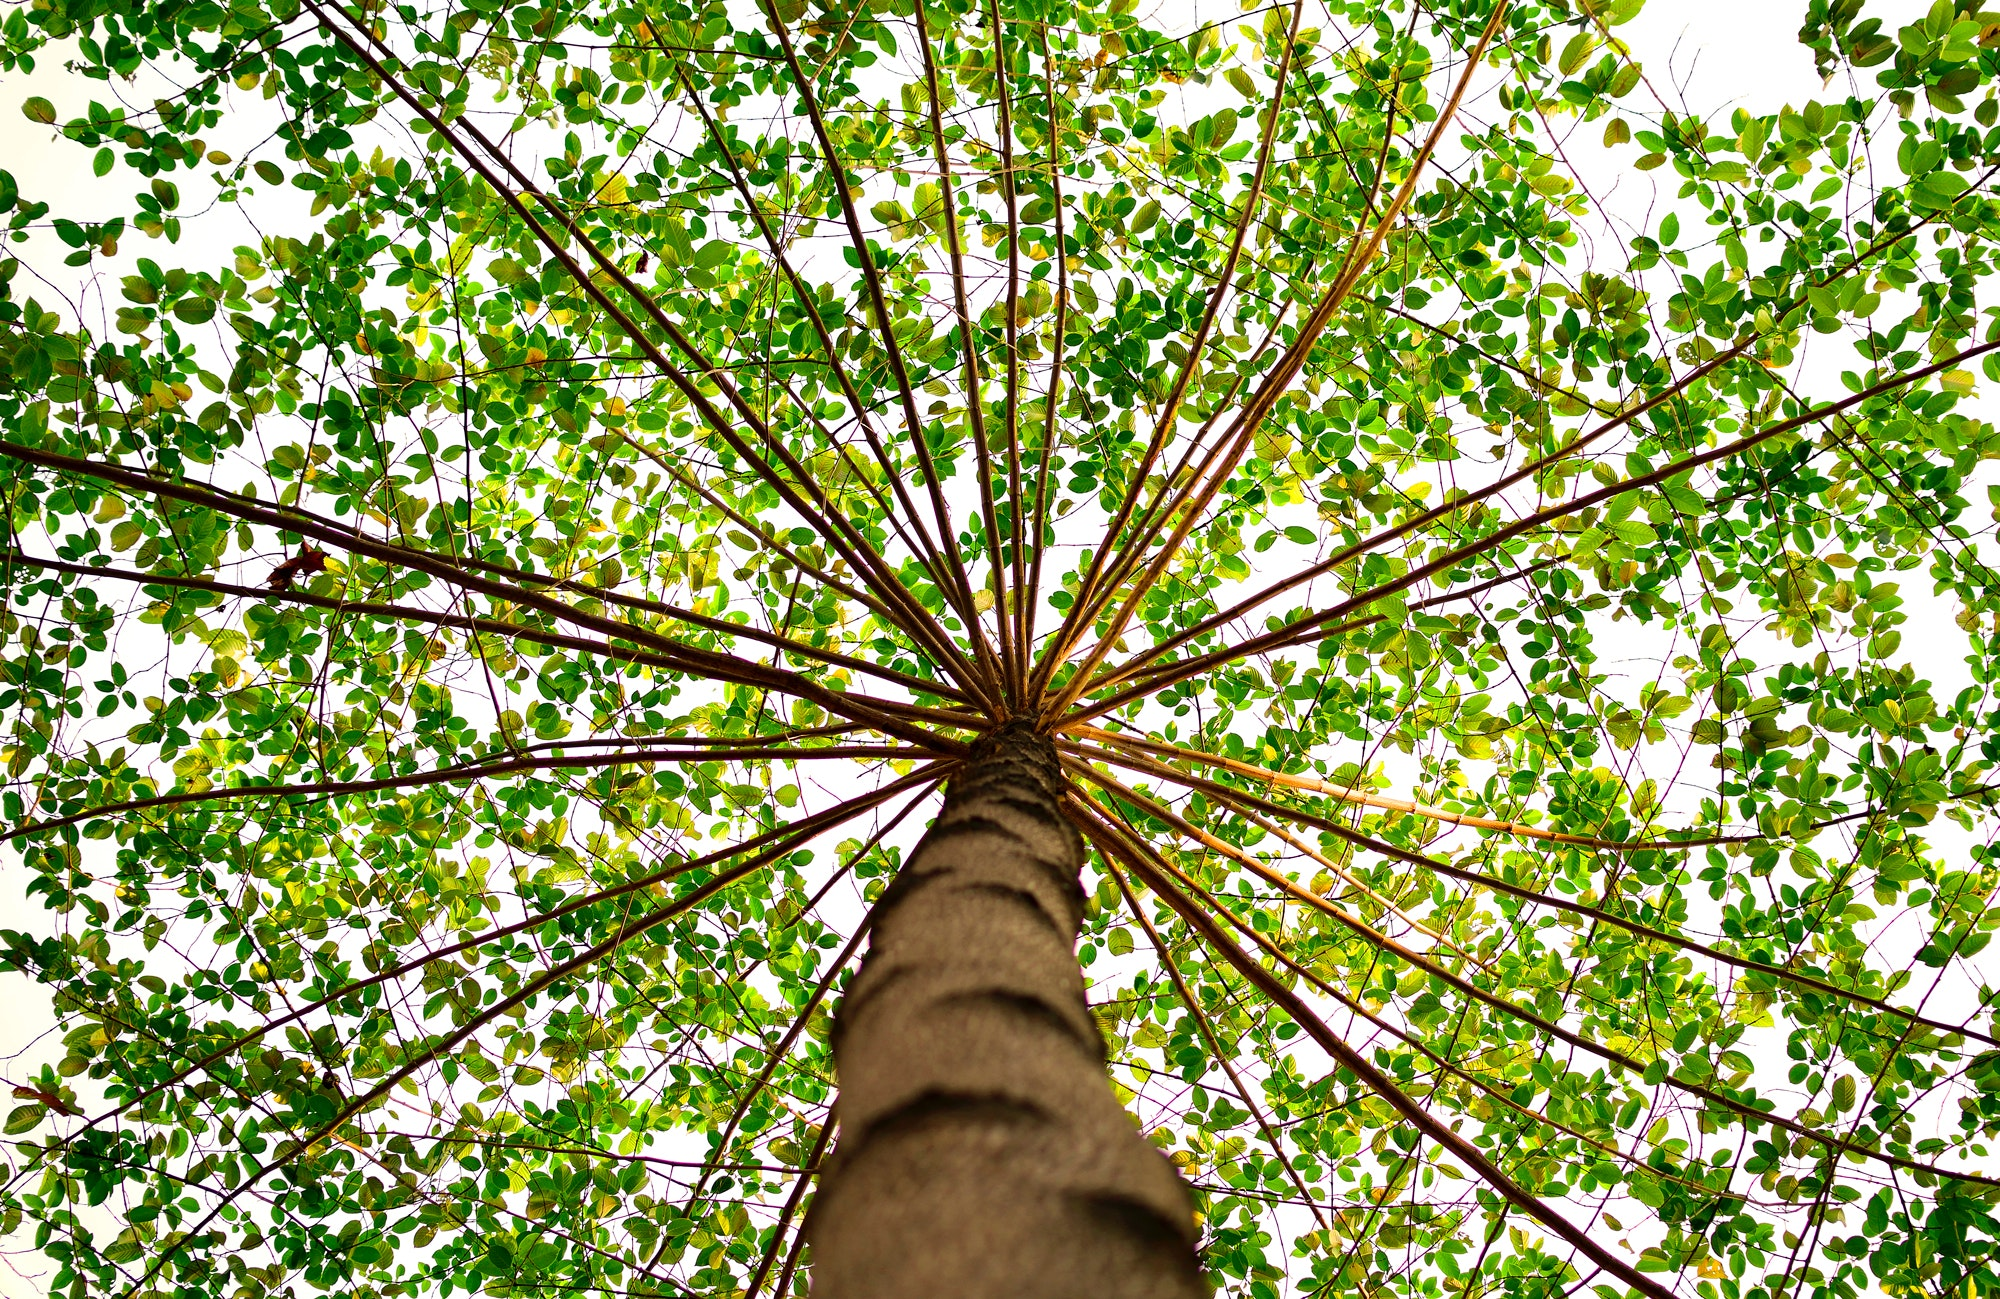
\includegraphics[width=0.7\textwidth]{figures/tree.jpg}\\
		\hspace*{15pt}\hbox{\scriptsize Image By:\thinspace{\itshape Lerkrat Tangsri}}
		%https://www.pexels.com/photo/wood-light-nature-forest-91153/
	\end{center}
	\pnote{We take a break from the problem for a bit}
\end{frame}

\begin{frame}
	\frametitle{General recursion tree}
	\begin{block}{Recurrence equation}
		For $a\geq 1$	and $b \geq 2$:\\
		$T(n) = \begin{cases}
			\Theta(1) & \text{if } n=1\\
			aT(n/b) + f(n) & \text{else}
		\end{cases}$
	\end{block}		
	\vspace{-5pt}
	\begin{figure}[htpb]
	\begin{center}
		\begin{tikzpicture}[scale=0.45, transform shape]

			\foreach \x in {0}{
				\node[draw, rectangle, fill=gray!10, minimum size = 0.4] (a\x) at (\x*8,8) {$T(n)$};
				\foreach \y in {0,...,2}{
					\node[draw,rectangle, fill=gray!10, minimum size =0.4] (b\y) at (-4+\x*8+\y*4,6) {$T(n/b)$};
					\draw (a\x) -- (b\y);
					\draw[dotted] (-6,7) -- node[fill=white] {$a$ calls} (6,7);
					\only<2->{
						\foreach \z in {0,...,2}{
							\ifthenelse{\y = 1}{
								\node[] (c\z) at (-1.5+\z*1.5,4.8) { };
								\draw[dashed] (b\y) -- (c\z);
								}{
								\node[draw,rectangle, fill=gray!10, minimum size =0.4] (c\z) at (-6+\x*8+\y*4+\z*2,4) {$T(n/b^2)$};
								\draw (b\y) -- (c\z);
								\foreach \a in {0,...,2}{
									\node[] (d\a) at (-6.5+\x*8+\y*4+\z*2+\a*0.5,2) { };
									\draw[dashed] (c\z) -- (d\a);
								}
							}
							\draw[dotted] (-5.5+\x*8+\y*4,5) -- node[fill=white] {$a$ calls} (-6+\x*8+\y*4+3.5,5);
						}
					}
				}
			}
			\node at (14, 0) { };

			\only<3->{
				\draw[fill=blue!60] (-8,2) rectangle node {$T(n/b^k)$} (7,3);
			}

			\only<4->{
				\foreach \x in {0,...,4}{
					\node[] (b\x) at (-7+\x*3,2) { };
					\node[draw, rectangle, fill=gray!10, minimum size = 0.4] (a\x) at (-8+\x*3,1) {$T(1)$};
					\draw[dotted] (b\x) -- (a\x);
				}

				\foreach \x in {0,...,4}{
					\node[] (b\x) at (-7+\x*3,2) { };
					\node[] (a\x) at (-7+\x*3,1) { };
					\draw[dotted] (b\x) -- (a\x);
				}

				\foreach \x in {0,...,4}{
					\node[] (b\x) at (-7+\x*3,2) { };
					\node[draw, rectangle, fill=gray!10, minimum size = 0.4] (a\x) at (-6+\x*3,1) {$T(1)$};
					\draw[dotted] (b\x) -- (a\x);
				}
			}

			\only<5->{
				\node at (9,9) {\Large Amount of nodes $\cdot$ combining};
				\node at (9,7.9) {\Large $1 \cdot f(n)$};
				\node at (9,5.9) {\Large $a \cdot f(n/b)$};
				\node at (9,3.9) {\Large $a^2 \cdot f(n/b^2)$};
			}

			\only<6->{
				\node at (9,2.3) {\Large $a^k \cdot f(n/b^k)$};
				\node at (9,1.2) {\Large $a^{\log_b n } \cdot f(1)$};
			}

			\only<7->{
				\draw (7,0.5) -- (11,0.5) node[anchor = west] {\Large $+$};
				\node at (9,-0.2) {\Large $\sum\limits_{i=0}^{log_b n} a^i \cdot f(\dfrac{n}{b^i})$};
			}

			\only<8->{
				\node[anchor=west] at (-7, -0.2) {\Large Total time spent in the leaves: $\Theta(a^{\log_b n}) = \Theta(n^{\log_b a})$.};
			}

			\only<9->{
				\node[red, anchor=west] at (5, -0.2) {\Large $\leq, =, \geq$};
				\node[red, anchor=west] at (4.7, -1.2) {\Large Which is it?};
			}

		\end{tikzpicture}
	\end{center}
\end{figure}

\end{frame}

\begin{frame}
	\frametitle{The master method}
	\begin{columns}[t]
		\column{0.455\textwidth}
	\begin{block}{Recurrence equation}
		For $a\geq 1$	and $b \geq 2$:\\
		$T(n) = \begin{cases}
			\Theta(1) & \text{if } n=1\\
			aT(n/b) + f(n) & \text{else}
		\end{cases}$
	\end{block}		
			
		\column{0.455\textwidth}

	\begin{answerblock}{From the tree}
		$T(n) = \Theta(n^{\log_b a}) + \sum\limits_{i=0}^{\log_b n} a^i\cdot f(\dfrac{n}{b^i})$, where:
		\begin{itemize}
			\item the first term represents the work in the leaves.
			\item the second term represents the work in combining the results.
		\end{itemize}
	\end{answerblock}
			
	\end{columns}

	\pause
	\hfill\\
	There are three common cases. The running time is: 
	\begin{enumerate}
		\item	dominated by \alert{the leaves}.
		\item	\alert{evenly distributed} throughout the tree.
		\item	dominated by \alert{the root}.
	\end{enumerate}

\end{frame}

\begin{frame}
	\frametitle{One method to rule them all}

	\begin{overlayarea}{\textwidth}{1.2\textheight}
		\begin{problemblock}{The recurrence equation}
			\scriptsize
			A recurrence equation in the form: $T(n) = a T(n/b) + f(n)$.
		\end{problemblock}
		
		\begin{answerblock}{The solution}
				\scriptsize
			Three common cases:
			\begin{enumerate}
				\item	dominated by \alert{the leaves}. \hfill\\
					If $f(n)$ is $O(n^{\log_b a - \epsilon})$, then $T(n)$ is $\Theta(n^{\log_b a})$. {\small\hfill for some $\epsilon > 0$}
				\item<2->	\alert{evenly distributed} throughout the tree.\hfill\\
					If $f(n)$ is $\Theta(n^{\log_b a})$, then $T(n)$ is $\Theta(n^{\log_b a} \log n)$. 
				\item<3->	dominated by \alert{the root}.\hfill\\
					If $f(n)$ is $\Omega(n^{\log_b a + \epsilon})$, then $T(n)$ is $ \Theta(f(n))$. {\small\hfill for some $\epsilon > 0$}
			\end{enumerate}	
		\end{answerblock}
		\only<3->{
			\begin{block}{Case 3 has a special requirements}
				\small
				Check the regularity condition: $a f(n/b) \leq c f(n)$. For some $c < 1$.\\
				Hint: Polynomials always satisfy this condition.
			\end{block}	
		}
	\end{overlayarea}
\end{frame}

\begin{frame}
	\frametitle{Let's do some examples}
	\framesubtitle{XKCD: \url{https://xkcd.com/189/}}

	\begin{center}
		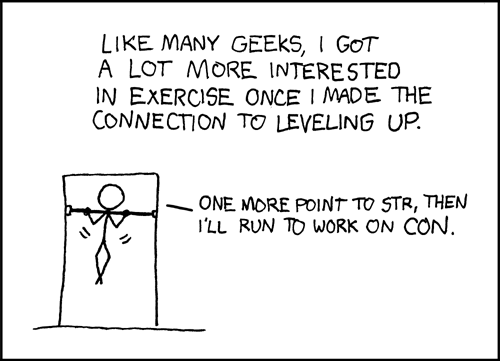
\includegraphics[width=0.7\textwidth]{figures/exercise.png}
	\end{center}
\end{frame}

%\begin{frame}
%	\frametitle{Example 2 - Merge sort}
%	\begin{overlayarea}{\textwidth}{\textheight}
%		\begin{block}{The method}
%			\small
%			\begin{itemize}
%				\item Identify $a$, $b$, $f(n)$ from a given recurrence equation.
%				\item Determine $n^{\log_b a}$.
%				\item Compare $n^{\log_b a}$ and $f(n)$.
%				\item Determine the right case from the master method and apply. 
%			\end{itemize}
%		\end{block}	
%		\only<2>{
%			\begin{problemblock}{Example 2 - Merge sort}
%				\small
%				$T(n) = 2 T(n/2) + \Theta(n)$	\\
%				Which part of the algorithm uses strictly more time?
%				\begin{enumerate}[A.]
%					\item Work in the leaves: $n^{\log_b a}$.
%					\item Work in the root node: $f(n)$.
%					\item Evenly spread throughout the tree.
%					\item We cannot apply the master method.
%				\end{enumerate}
%			\end{problemblock}
%		}
%		\only<3>{
%			\begin{answerblock}{Example 2 - Merge sort}
%				\small
%				$T(n) = 2 T(n/2) + \Theta(n)$	\\
%				$a = 2, b =2, n^{\log_b a} = n^{\log_2 2} = n$\\
%				$f(n)$ is $\Theta(n)$\\
%				So case 2 of the master method, thus $T(n)$ is $\Theta(n^{\log_2 2} \log n) =\Theta(n \log n)$.
%			\end{answerblock}
%		}
%	\end{overlayarea}
%\end{frame}

\begin{frame}
	\frametitle{Example 1 - Binary Search}
	\framesubtitle{From last week}
	\begin{overlayarea}{\textwidth}{\textheight}
		\begin{columns}
			\column{0.455\textwidth}
				
		\begin{algorithmic}
			\scriptsize
			\Function{Binary-Search}{A,p,q,r,s}
			\State $q \gets (p+r)/2$
			\If{$p > r$}
			\State \Return false
			\ElsIf{$a[q] = s$}
			\State \Return $q$
			\ElsIf{$a[q] > s$}
			\State \Return \Call{Binary-Search}{a,p,q-1,s}
			\Else
			\State \Return \Call{Binary-Search}{a,q+1,r,s}
			\EndIf
			\EndFunction
		\end{algorithmic}
			\column{0.455\textwidth}
				
		\only<3->{
			\begin{problemblock}{Example 1 - Binary search}
				Which part of the algorithm uses strictly more time?
				\begin{enumerate}[A.]
					\small
					\item Work in the leaves: $n^{\log_b a}$.
					\item Work in the root node: $f(n)$.
					\item Evenly spread throughout the tree.
					\item We cannot apply the master method.
				\end{enumerate}
			\end{problemblock}
		}
		\only<2>{
			\begin{problemblock}{Example 1 - Binary search}
				So what is the recurrence equation again?
					\begin{enumerate}[A.]
						\item $T(n) = T(n/2) + c$
						\item $T(n) = T(n/2) + n$
						\item $T(n) = 2T(n/2) + c$
						\item $T(n) = 2T(n/2) + n$
						\item $T(n) = 2T(n/2) + n\log n$
						\item I don't know.
					\end{enumerate}
			\end{problemblock}
		}
		\end{columns}
		\only<4>{
			\begin{answerblock}{Example 1 - Binary search}
				\small
				$T(n) = T(n/2) + \Theta(1)$	\\
				$a = 1, b =2, n^{\log_b a} = n^{\log_2 1} = n^0 = 1$\\
				$f(n)$ is $\Theta(1)$\\
				So case 2 of the master method, thus $T(n)$ is $\Theta(n^{\log_2 1} \log n) =\Theta(\log n)$.
			\end{answerblock}
		}
	\end{overlayarea}
\end{frame}

\begin{frame}
	\frametitle{Example 2 - 9 \st{rings} calls}
	\begin{overlayarea}{\textwidth}{\textheight}
		\begin{problemblock}{Example 2}
			\small
			$T(n) = 9 T(n/3) + n$	\\
			\only<1>{
				Which part of the algorithm uses strictly more time?
				\begin{enumerate}[A.]
					\item Work in the leaves: $n^{\log_b a}$.
					\item Work in the root node: $f(n)$.
					\item Evenly spread throughout the tree.
					\item We cannot apply the master method.
				\end{enumerate}
			}
		\end{problemblock}
		\only<2>{
			\begin{answerblock}{Example 2}
				\small
				$a = 9, b =3, n^{\log_b a} = n^{\log_3 9} = n^2$\\
				$f(n)$ is $\Theta(n)$\\
				So case 1 of the master method (most work is in the leaves), \\
				thus $T(n)$ is $\Theta(n^{\log_9 3}) =\Theta(n^2)$.
			\end{answerblock}
		}
	\end{overlayarea}
\end{frame}

\begin{frame}
	\frametitle{Example 3 - Worse binary recursion}
	\begin{overlayarea}{\textwidth}{\textheight}
		\begin{problemblock}{Example 3 - Worse binary recursion}
			$T(n) = T(n/2) + n$
			\only<1>{
				So what is the run time?
				\begin{multicols}{2}
					\begin{enumerate}[A.]
						\item $T(n) $ is $O(n)$.
						\item $T(n) $ is $O(n \log n)$.
						\item $T(n) $ is $O(n^2)$.
						\item $T(n) $ is $O(n^2 \log n)$.
						\item $T(n) $ is $O(n^3)$.
						\item I don't know.
					\end{enumerate}
				\end{multicols}
			}
		\end{problemblock}
		\only<2->{
			\begin{answerblock}{Example 3}
				\small
				$T(n) = T(n/2) + \Theta(n)$	\\
				$a = 1, b =2, n^{\log_b a} = n^{\log_2 1} = n^0 = 1$\\
				$f(n)$ is $\Theta(n)$\\
				So case 3 of the master method, thus $T(n)$ is $\Theta(f(n)) =\Theta(n)$.
				\only<3>{
					\alert{Or is it?}
				}
				\only<4->{
					check regularity condition! Do one of the following:
					\begin{itemize}
						\item observe that $f(n)$ is a polynomial function
						\item observe that $a f(n/b) \leq c f(n)$ for some $c < 1$, in this case: $f(n/2) = n/2 \leq 0.5 n = 0.5
							f(n)$ so for $c = 0.5$
					\end{itemize}
				}
			\end{answerblock}
		}
	\end{overlayarea}
\end{frame}

\begin{frame}
	\frametitle{Example 4 - Multiplying matrices}
	\framesubtitle{From last weeks intermezzo}
	\begin{overlayarea}{\textwidth}{\textheight}
		\begin{problemblock}{Example 4 - Multiplying matrices}
			$T(n) = 7T(n/2) + n^2$
			\only<1>{
				So what is the run time?
				\begin{multicols}{2}
					\begin{enumerate}[A.]
						\item $T(n) $ is $O(n)$.
						\item $T(n) $ is $O(n \log n)$.
						\item $T(n) $ is $O(n^2)$.
						\item $T(n) $ is $O(n^2 \log n)$.
						\item $T(n) $ is $O(n^3)$.
						\item I don't know.
					\end{enumerate}
				\end{multicols}
			}
		\end{problemblock}
		\only<2->{
			\begin{answerblock}{Case ...?}
				\small
				$a = 7, b =2, n^{\log_b a} = n^{\log_2 7} \approx n^{2.81}$\\
				$f(n)$ is $\Theta(n^2)$\\
				\pause
				$f(n)$ is $O(n^{2.81-\epsilon})$ so case 1 (dominated by the leaves)\\
				So $T(n)$ is $\Theta(n^{\log_b a}) \approx \Theta(n^{2.81})$
			\end{answerblock}
		}
	\end{overlayarea}
\end{frame}


\section{Back to closest pair of points}
\label{sec:back_to_closest_pair_of_points}


\begin{frame}
	\frametitle{The algorithm}
	\begin{columns}
		\column{0.705\textwidth}
	\begin{algorithmic}
		\State Sort all points by x-coordinate
		\Function{Closest-Pair}{$p_1,\dots,p_n$}
			\If{n=1}
				\State \Return $\infty$
			\EndIf

			\State $L \gets$ \alert<2>{median} $x$-coordinate
			\State $\delta_1 \gets$ \Call{Closest-Pair}{Points left of $L$}
			\State $\delta_2 \gets$ \Call{Closest-Pair}{Points right of $L$}
			\State $\delta \gets \min(\delta_1,\delta_2)$
			\State get list of all points within $\delta$ from L.
			\State sort this list by y-coordinate
			\State Scan by y-order, compare every point to the next 11 and update $\delta$ as you go.
			\State \Return $\delta$
		\EndFunction
	\end{algorithmic}
		\pnote{Why not the average?}
		\column{0.205\textwidth}
		\begin{questionblock}{}
			What is the recurrence equation for the run time?	
		\end{questionblock}	
		\begin{answerblock}{}
			\small
			$T(n) =2T(n/2) + O(n\log n)$	
		\end{answerblock}
	\end{columns}
	
\end{frame}

\begin{frame}
	\frametitle{Back to closest pair of points}
	\section{Closest pair of points}
\label{sec:closest_pair_of_points}


\begin{frame}
	\frametitle{A new problem}
	\begin{problemblock}{Closest pair of points}
		Given a set of points, what is the pair of points that is closest to each other?\\
		\pause
		More formally:
		\begin{itemize}
			\item Given a set of points $S$, where every point $p_i$ has an x-coordinate $x_i$ and y-coordinate $y_i$.
			\item Distance is defined as: $d(i,j) = \sqrt{{(x_i - x_j)}^{2} + {(y_i-y_j)}^2}$
			\item What is the pair of points $i,j$ such that $d(i,j)$ is minimal?
		\end{itemize}
	\end{problemblock}
	\pause
	\section{Closest pair of points}
\label{sec:closest_pair_of_points}


\begin{frame}
	\frametitle{A new problem}
	\begin{problemblock}{Closest pair of points}
		Given a set of points, what is the pair of points that is closest to each other?\\
		\pause
		More formally:
		\begin{itemize}
			\item Given a set of points $S$, where every point $p_i$ has an x-coordinate $x_i$ and y-coordinate $y_i$.
			\item Distance is defined as: $d(i,j) = \sqrt{{(x_i - x_j)}^{2} + {(y_i-y_j)}^2}$
			\item What is the pair of points $i,j$ such that $d(i,j)$ is minimal?
		\end{itemize}
	\end{problemblock}
	\pause
	\input{figures/tikz/closestpair.tex}
	\pnote{Why is this relevant? Answers: For instance collision detection algorithms}
\end{frame}

\begin{frame}
	\frametitle{Let's just brute-force it?}
	\begin{overlayarea}{\textwidth}{\textheight}
		\input{figures/tikz/closestpair.tex}
		\begin{questionblock}{Brute-force}
			What is the tightest upper bound on the run time for a brute-force solution given $|S| = n$?
			\only<2>{
			\begin{enumerate}[A.]
				\item $O(n \log n)$
				\item $O(n^2)$
				\item $O(n^2 \log n)$
				\item $O(n^3)$
				\item I don't know.
			\end{enumerate}
		}
		\end{questionblock}
		\only<3>{
			\begin{answerblock}{Try every combination}
				We check every pair of points, of which there are $n^2$, so $O(n^2)$.	
			\end{answerblock}
		}
	\end{overlayarea}
\end{frame}

\begin{frame}
	\frametitle{Time to improve!}
	\framesubtitle{Using Divide \& Conquer}
		\begin{columns}
			\column{0.455\textwidth}
			\begin{center}
				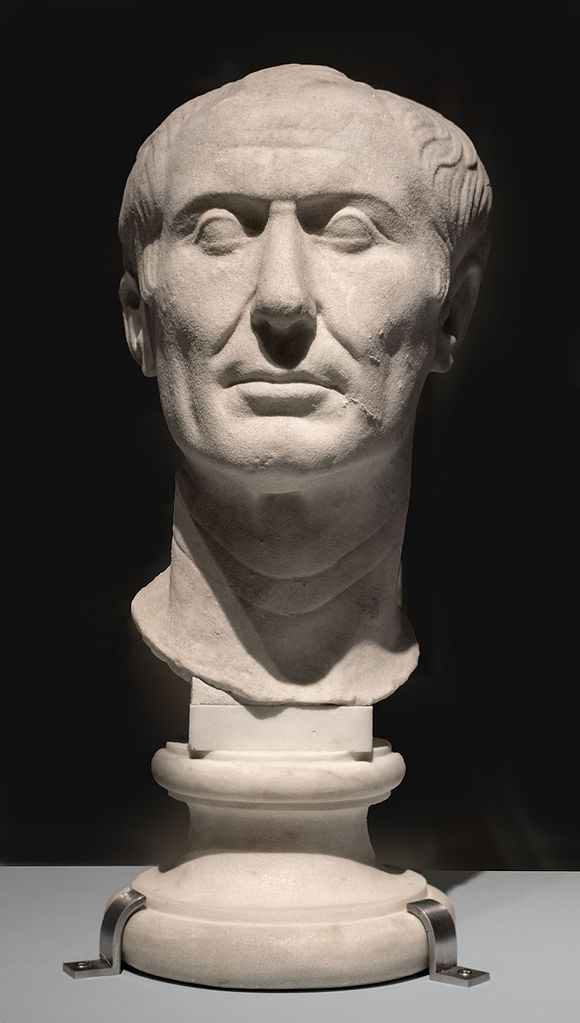
\includegraphics[width=0.5\textwidth]{figures/ceasar.jpg}\\
				\hspace*{15pt}\hbox{\scriptsize Image By:\thinspace{\itshape Ángel M. Felicísimo}}
				%https://commons.wikimedia.org/wiki/File:Retrato_de_Julio_C%C3%A9sar_(26724093101).jpg
			\end{center}

			\column{0.455\textwidth}
			\begin{center}
				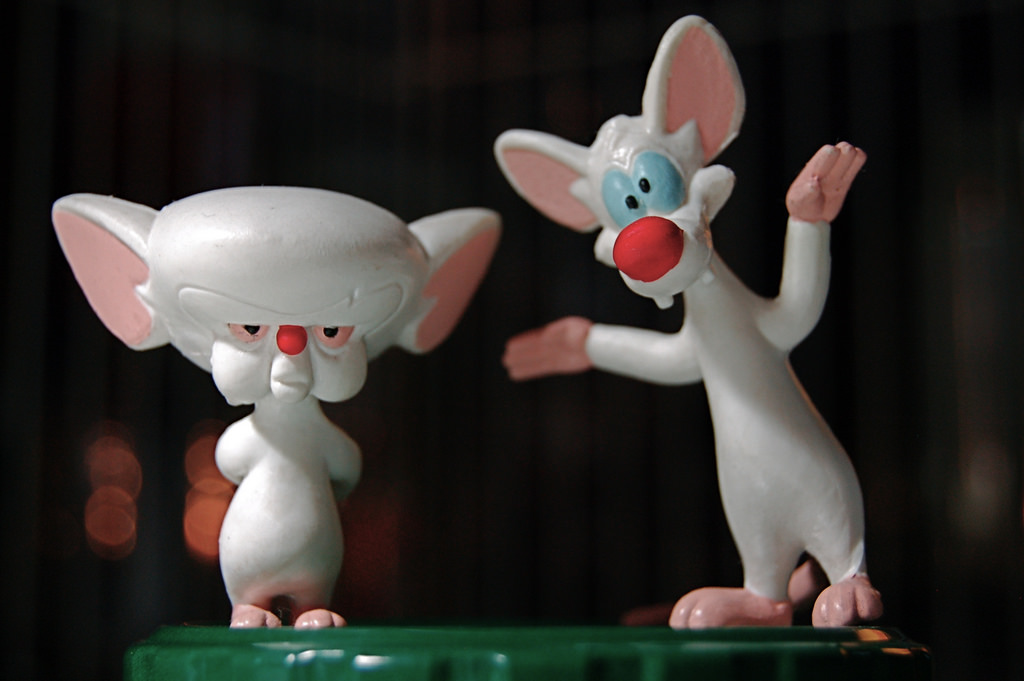
\includegraphics[width=0.9\textwidth]{figures/pinky.jpg}\\
				\hspace*{15pt}\hbox{\scriptsize Image By:\thinspace{\itshape JD Hancock}}
				%https://commons.wikimedia.org/wiki/File:Retrato_de_Julio_C%C3%A9sar_(26724093101).jpg

			\end{center}
		\end{columns}
\end{frame}

\begin{frame}
	\frametitle{Ideas for an algorithm}

	\begin{overlayarea}{\textwidth}{\textheight}
		\input{figures/tikz/closestpair_fixed.tex}
		
		\pause
		\begin{exampleblock}{Algorithm}
			\begin{itemize}
				\item \alert<2>{Divide}: Draw vertical line $L$ that has roughly half of the points on each side.
					\pause
				\item \alert<3>{Conquer}: Find the closest pair on each side.
					\pause
				\item \alert<4>{Combine}: Find the closest pair with one point on each side.
					\pause
				\item Return the minimum of these 3.
			\end{itemize}
		\end{exampleblock}	
	\end{overlayarea}
\end{frame}

\begin{frame}
	\frametitle{Did we make things better?}
	\begin{questionblock}{What is the run time of combine?}
		How much time to combine the two halves? Remember that we want to improve over $\Theta(n^2)$.
	\end{questionblock}	
\end{frame}

\begin{frame}
	\frametitle{How do we make it better?}
		\input{figures/tikz/closestpair_fixed2.tex}
	Observation:
	\begin{itemize}
		\item If $\delta$ is the minimum of the smallest distances left and right.
			\pause
		\item Then we only need to consider pairs of points within $\delta$ of $L$.
			\pause
		\item So in this example, none at all!
	\end{itemize}
\end{frame}

\begin{frame}
	\frametitle{Worst-case?}
	\begin{overlayarea}{\textwidth}{\textheight}
			\begin{itemize}
				\item But worst-case all points are in this $2\delta$-strip...
					\pause
				\item But if we sort them by $y$-coordinate (which can be done in $O(n\log n)$), then how many comparisons do we need?
					\pause
				\item Still $O(n^2)$!?
					\only<4->{
				\item Nope! We only need to check within 11 (i.e. a constant number of) positions in the sorted list.
				}
					\only<5->{
				\item So the combining step is $O(n \log n)$ (which can be further improved to $O(n)$)!
				}
			\end{itemize}
			\only<3>{
			\begin{center}
				
\includegraphics[width=0.4\textwidth]{figures/dilbert.jpg}
				\framesubtitle{http://thecontextofthings.com/wp-content/uploads/2017/11/dilbert-work.jpg}
			\end{center}
		}
	\end{overlayarea}
\end{frame}

\begin{frame}
	\frametitle{Why 11?}

	\begin{overlayarea}{\textwidth}{\textheight}
		\begin{columns}
			\column{0.655\textwidth}
			\begin{block}{Definition}
				Let $s_i$ be the point in the $2\delta$-strip with the $i^\text{th}$ smallest $y$-coordinate.
			\end{block}	
			
			\pause
			\begin{block}{Claim about 11}
				If $|i-j| > 11$ then the distance between $s_i$ and $s_j$ is at least $\delta$.
			\end{block}
			\column{0.255\textwidth}
			\input{figures/tikz/closestpair_delta.tex}	
		\end{columns}
		
		\pause
		\only<3-5>{
			\begin{block}{Proof sketch}
			\begin{itemize}
				\item No two points are in the same $0.5\delta$-by-$0.5\delta$-box.
					\only<4->{
				\item Two points that have two rows between them have a distance $\geq 2\cdot(0.5\delta) = \delta$.
				}
				\only<5->{
				\item So we only consider points at most 2 rows away.
				}
			\end{itemize}
		\end{block}
	}
	\only<6->{
		\begin{exampleblock}{Fun facts!}
			\begin{itemize}
				\item We can even reduce this to just 7 points.
					\only<7>{
				\item Even less if we consider columns separately.
				}
			\end{itemize}
		\end{exampleblock}	
	}
		
		\only<3>{
		\begin{questionblock}{Why not?}
			Why are there no two points in the same box?
		\end{questionblock}
}
	\end{overlayarea}
\end{frame}

\begin{frame}
	\frametitle{The algorithm}
	\begin{columns}
		\column{0.705\textwidth}
	\begin{algorithmic}
		\State Sort all points by x-coordinate
		\Function{Closest-Pair}{$p_1,\dots,p_n$}
			\If{n=1}
				\State \Return $\infty$
			\EndIf

			\pause
			\State $L \gets$ \alert<2>{median} $x$-coordinate
			\State $\delta_1 \gets$ \Call{Closest-Pair}{Points left of $L$}
			\State $\delta_2 \gets$ \Call{Closest-Pair}{Points right of $L$}
			\State $\delta \gets \min(\delta_1,\delta_2)$
			\pause
			\State get list of all points within $\delta$ from L.
			\State sort this list by y-coordinate
			\pause
			\State Scan by y-order, compare every point to the next 11 and update $\delta$ as you go.
			\State \Return $\delta$
		\EndFunction
	\end{algorithmic}
		\pnote{Why not the average?}
		\column{0.205\textwidth}
		\pause
		\begin{questionblock}{}
			What is the recurrence equation for the run time?	
		\end{questionblock}	
		\pause
		\begin{answerblock}{}
			\small
			$T(n) =2T(n/2) + O(n\log n)$	
		\end{answerblock}
	\end{columns}
	
\end{frame}

	\pnote{Why is this relevant? Answers: For instance collision detection algorithms}
\end{frame}

\begin{frame}
	\frametitle{Let's just brute-force it?}
	\begin{overlayarea}{\textwidth}{\textheight}
		\section{Closest pair of points}
\label{sec:closest_pair_of_points}


\begin{frame}
	\frametitle{A new problem}
	\begin{problemblock}{Closest pair of points}
		Given a set of points, what is the pair of points that is closest to each other?\\
		\pause
		More formally:
		\begin{itemize}
			\item Given a set of points $S$, where every point $p_i$ has an x-coordinate $x_i$ and y-coordinate $y_i$.
			\item Distance is defined as: $d(i,j) = \sqrt{{(x_i - x_j)}^{2} + {(y_i-y_j)}^2}$
			\item What is the pair of points $i,j$ such that $d(i,j)$ is minimal?
		\end{itemize}
	\end{problemblock}
	\pause
	\input{figures/tikz/closestpair.tex}
	\pnote{Why is this relevant? Answers: For instance collision detection algorithms}
\end{frame}

\begin{frame}
	\frametitle{Let's just brute-force it?}
	\begin{overlayarea}{\textwidth}{\textheight}
		\input{figures/tikz/closestpair.tex}
		\begin{questionblock}{Brute-force}
			What is the tightest upper bound on the run time for a brute-force solution given $|S| = n$?
			\only<2>{
			\begin{enumerate}[A.]
				\item $O(n \log n)$
				\item $O(n^2)$
				\item $O(n^2 \log n)$
				\item $O(n^3)$
				\item I don't know.
			\end{enumerate}
		}
		\end{questionblock}
		\only<3>{
			\begin{answerblock}{Try every combination}
				We check every pair of points, of which there are $n^2$, so $O(n^2)$.	
			\end{answerblock}
		}
	\end{overlayarea}
\end{frame}

\begin{frame}
	\frametitle{Time to improve!}
	\framesubtitle{Using Divide \& Conquer}
		\begin{columns}
			\column{0.455\textwidth}
			\begin{center}
				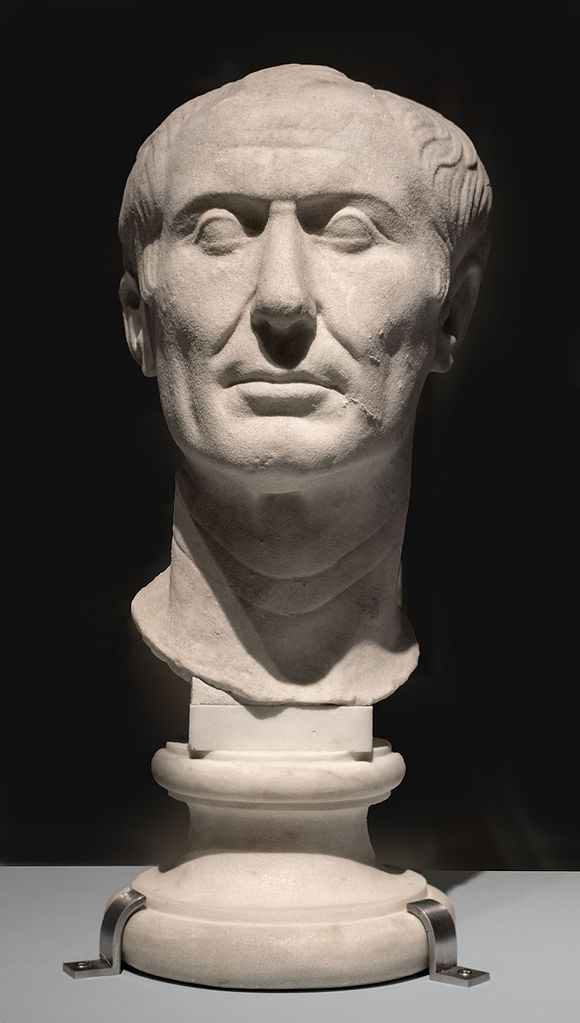
\includegraphics[width=0.5\textwidth]{figures/ceasar.jpg}\\
				\hspace*{15pt}\hbox{\scriptsize Image By:\thinspace{\itshape Ángel M. Felicísimo}}
				%https://commons.wikimedia.org/wiki/File:Retrato_de_Julio_C%C3%A9sar_(26724093101).jpg
			\end{center}

			\column{0.455\textwidth}
			\begin{center}
				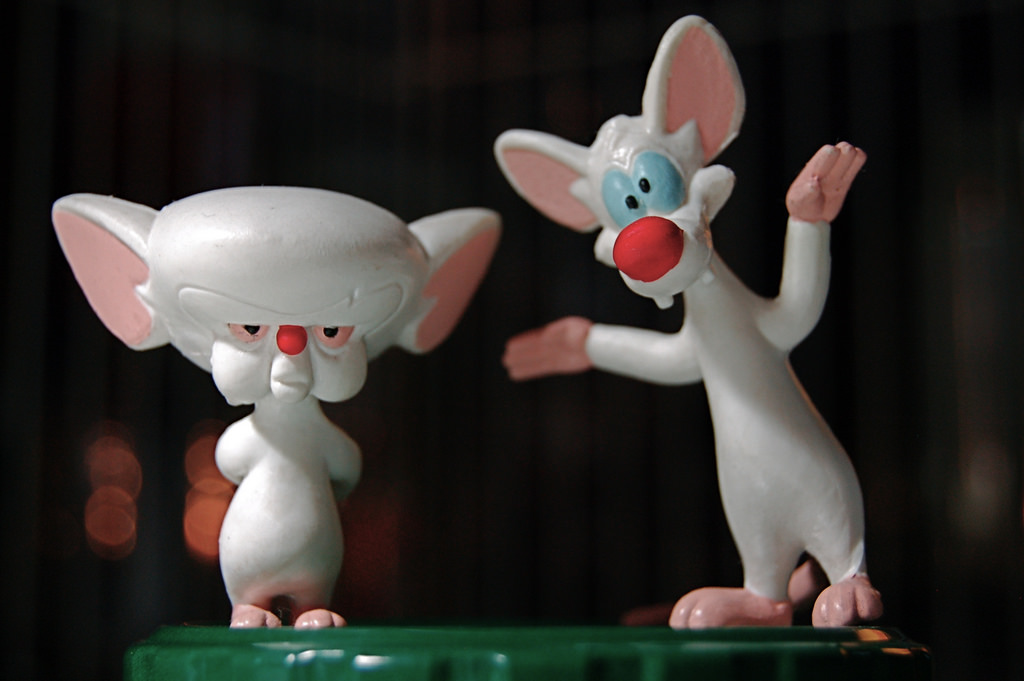
\includegraphics[width=0.9\textwidth]{figures/pinky.jpg}\\
				\hspace*{15pt}\hbox{\scriptsize Image By:\thinspace{\itshape JD Hancock}}
				%https://commons.wikimedia.org/wiki/File:Retrato_de_Julio_C%C3%A9sar_(26724093101).jpg

			\end{center}
		\end{columns}
\end{frame}

\begin{frame}
	\frametitle{Ideas for an algorithm}

	\begin{overlayarea}{\textwidth}{\textheight}
		\input{figures/tikz/closestpair_fixed.tex}
		
		\pause
		\begin{exampleblock}{Algorithm}
			\begin{itemize}
				\item \alert<2>{Divide}: Draw vertical line $L$ that has roughly half of the points on each side.
					\pause
				\item \alert<3>{Conquer}: Find the closest pair on each side.
					\pause
				\item \alert<4>{Combine}: Find the closest pair with one point on each side.
					\pause
				\item Return the minimum of these 3.
			\end{itemize}
		\end{exampleblock}	
	\end{overlayarea}
\end{frame}

\begin{frame}
	\frametitle{Did we make things better?}
	\begin{questionblock}{What is the run time of combine?}
		How much time to combine the two halves? Remember that we want to improve over $\Theta(n^2)$.
	\end{questionblock}	
\end{frame}

\begin{frame}
	\frametitle{How do we make it better?}
		\input{figures/tikz/closestpair_fixed2.tex}
	Observation:
	\begin{itemize}
		\item If $\delta$ is the minimum of the smallest distances left and right.
			\pause
		\item Then we only need to consider pairs of points within $\delta$ of $L$.
			\pause
		\item So in this example, none at all!
	\end{itemize}
\end{frame}

\begin{frame}
	\frametitle{Worst-case?}
	\begin{overlayarea}{\textwidth}{\textheight}
			\begin{itemize}
				\item But worst-case all points are in this $2\delta$-strip...
					\pause
				\item But if we sort them by $y$-coordinate (which can be done in $O(n\log n)$), then how many comparisons do we need?
					\pause
				\item Still $O(n^2)$!?
					\only<4->{
				\item Nope! We only need to check within 11 (i.e. a constant number of) positions in the sorted list.
				}
					\only<5->{
				\item So the combining step is $O(n \log n)$ (which can be further improved to $O(n)$)!
				}
			\end{itemize}
			\only<3>{
			\begin{center}
				
\includegraphics[width=0.4\textwidth]{figures/dilbert.jpg}
				\framesubtitle{http://thecontextofthings.com/wp-content/uploads/2017/11/dilbert-work.jpg}
			\end{center}
		}
	\end{overlayarea}
\end{frame}

\begin{frame}
	\frametitle{Why 11?}

	\begin{overlayarea}{\textwidth}{\textheight}
		\begin{columns}
			\column{0.655\textwidth}
			\begin{block}{Definition}
				Let $s_i$ be the point in the $2\delta$-strip with the $i^\text{th}$ smallest $y$-coordinate.
			\end{block}	
			
			\pause
			\begin{block}{Claim about 11}
				If $|i-j| > 11$ then the distance between $s_i$ and $s_j$ is at least $\delta$.
			\end{block}
			\column{0.255\textwidth}
			\input{figures/tikz/closestpair_delta.tex}	
		\end{columns}
		
		\pause
		\only<3-5>{
			\begin{block}{Proof sketch}
			\begin{itemize}
				\item No two points are in the same $0.5\delta$-by-$0.5\delta$-box.
					\only<4->{
				\item Two points that have two rows between them have a distance $\geq 2\cdot(0.5\delta) = \delta$.
				}
				\only<5->{
				\item So we only consider points at most 2 rows away.
				}
			\end{itemize}
		\end{block}
	}
	\only<6->{
		\begin{exampleblock}{Fun facts!}
			\begin{itemize}
				\item We can even reduce this to just 7 points.
					\only<7>{
				\item Even less if we consider columns separately.
				}
			\end{itemize}
		\end{exampleblock}	
	}
		
		\only<3>{
		\begin{questionblock}{Why not?}
			Why are there no two points in the same box?
		\end{questionblock}
}
	\end{overlayarea}
\end{frame}

\begin{frame}
	\frametitle{The algorithm}
	\begin{columns}
		\column{0.705\textwidth}
	\begin{algorithmic}
		\State Sort all points by x-coordinate
		\Function{Closest-Pair}{$p_1,\dots,p_n$}
			\If{n=1}
				\State \Return $\infty$
			\EndIf

			\pause
			\State $L \gets$ \alert<2>{median} $x$-coordinate
			\State $\delta_1 \gets$ \Call{Closest-Pair}{Points left of $L$}
			\State $\delta_2 \gets$ \Call{Closest-Pair}{Points right of $L$}
			\State $\delta \gets \min(\delta_1,\delta_2)$
			\pause
			\State get list of all points within $\delta$ from L.
			\State sort this list by y-coordinate
			\pause
			\State Scan by y-order, compare every point to the next 11 and update $\delta$ as you go.
			\State \Return $\delta$
		\EndFunction
	\end{algorithmic}
		\pnote{Why not the average?}
		\column{0.205\textwidth}
		\pause
		\begin{questionblock}{}
			What is the recurrence equation for the run time?	
		\end{questionblock}	
		\pause
		\begin{answerblock}{}
			\small
			$T(n) =2T(n/2) + O(n\log n)$	
		\end{answerblock}
	\end{columns}
	
\end{frame}

		\begin{questionblock}{Brute-force}
			What is the tightest upper bound on the run time for a brute-force solution given $|S| = n$?
			\only<2>{
			\begin{enumerate}[A.]
				\item $O(n \log n)$
				\item $O(n^2)$
				\item $O(n^2 \log n)$
				\item $O(n^3)$
				\item I don't know.
			\end{enumerate}
		}
		\end{questionblock}
		\only<3>{
			\begin{answerblock}{Try every combination}
				We check every pair of points, of which there are $n^2$, so $O(n^2)$.	
			\end{answerblock}
		}
	\end{overlayarea}
\end{frame}

\begin{frame}
	\frametitle{Time to improve!}
	\framesubtitle{Using Divide \& Conquer}
		\begin{columns}
			\column{0.455\textwidth}
			\begin{center}
				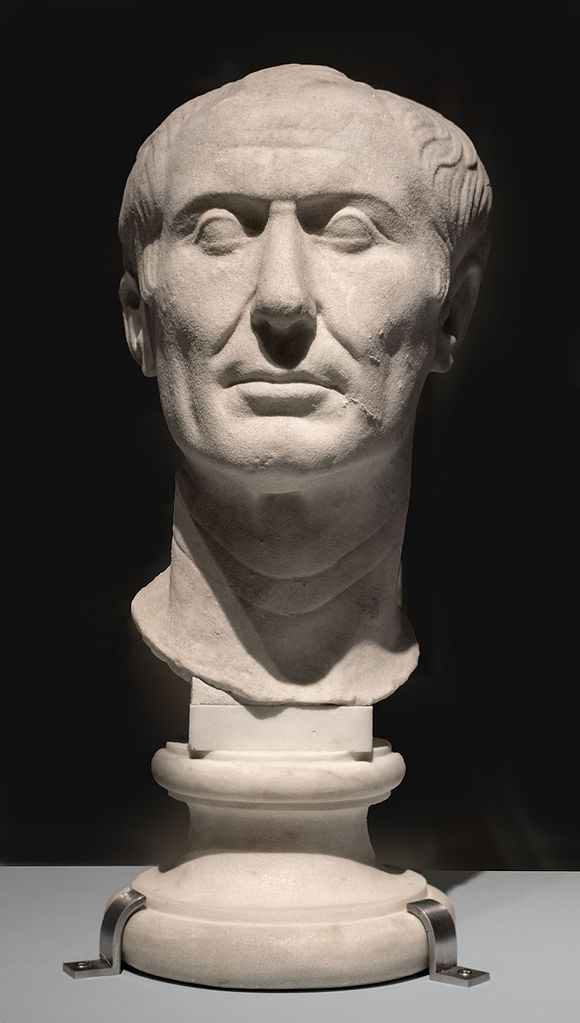
\includegraphics[width=0.5\textwidth]{figures/ceasar.jpg}\\
				\hspace*{15pt}\hbox{\scriptsize Image By:\thinspace{\itshape Ángel M. Felicísimo}}
				%https://commons.wikimedia.org/wiki/File:Retrato_de_Julio_C%C3%A9sar_(26724093101).jpg
			\end{center}

			\column{0.455\textwidth}
			\begin{center}
				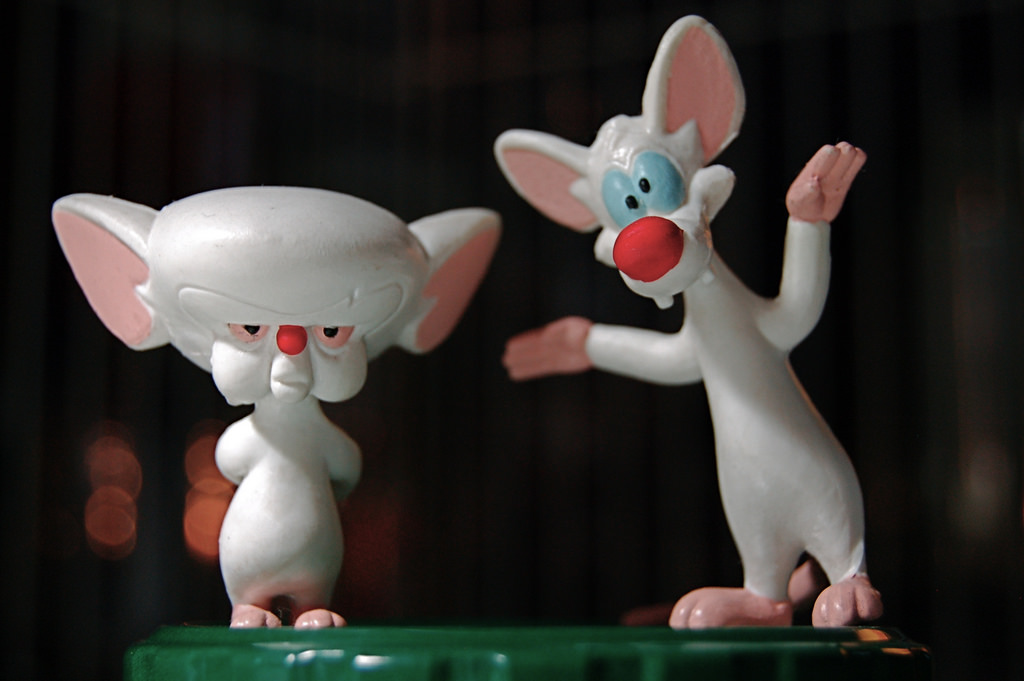
\includegraphics[width=0.9\textwidth]{figures/pinky.jpg}\\
				\hspace*{15pt}\hbox{\scriptsize Image By:\thinspace{\itshape JD Hancock}}
				%https://commons.wikimedia.org/wiki/File:Retrato_de_Julio_C%C3%A9sar_(26724093101).jpg

			\end{center}
		\end{columns}
\end{frame}

\begin{frame}
	\frametitle{Ideas for an algorithm}

	\begin{overlayarea}{\textwidth}{\textheight}
		\begin{figure}[htpb]
\begin{center}
\begin{tikzpicture}[scale=0.5, transform shape]
	\draw (-8,-3) rectangle (8,3);

	\foreach \x/\y/\name in {
		-7/2/,
		-6/1/l1,
		-5/1/l2,
		-3/-2/c1,
		-1/-2/c2,
		3/-1/,
		5/1.5/r1,
		5/0/r2,
		}{
		\node[circle, black, draw, fill=blue!30, minimum size=4pt] (\name) at (\x,\y) {};
	}
		\node at (-1.5, -3.5) {};
	\only<2->{
		\draw[dotted] (-1.5,-3) -- (-1.5,3);
		\node at (-1.5, -3.5) {\Large $L$};
	}
	\only<3->{
		\draw[dotted, red, thick] (l1) --  node[anchor=south] {\Large 1} (l2);
		\draw[dotted, red, thick] (r1) --  node[anchor=west] {\Large 1.5} (r2);
	}
	\only<4->{
		\draw[dotted, red, thick] (c1) --  node[anchor=south] {\Large 2} (c2);
	}
\end{tikzpicture}
\end{center}
\end{figure}

		
		\pause
		\begin{exampleblock}{Algorithm}
			\begin{itemize}
				\item \alert<2>{Divide}: Draw vertical line $L$ that has roughly half of the points on each side.
					\pause
				\item \alert<3>{Conquer}: Find the closest pair on each side.
					\pause
				\item \alert<4>{Combine}: Find the closest pair with one point on each side.
					\pause
				\item Return the minimum of these 3.
			\end{itemize}
		\end{exampleblock}	
	\end{overlayarea}
\end{frame}

\begin{frame}
	\frametitle{Did we make things better?}
	\begin{questionblock}{What is the run time of combine?}
		How much time to combine the two halves? Remember that we want to improve over $\Theta(n^2)$.
	\end{questionblock}	
\end{frame}

\begin{frame}
	\frametitle{How do we make it better?}
		\begin{figure}[htpb]
\begin{center}
\begin{tikzpicture}[scale=0.5, transform shape]
	\draw (-8,-3) rectangle (8,3);

	\only<2->{
		\draw[fill=gray!10] (-2.5,-3) rectangle (-0.5,3);
	}
	\foreach \x/\y/\name in {
		-7/2/,
		-6/1/l1,
		-5/1/l2,
		-3/-2/c1,
		-1/-2/c2,
		3/-1/,
		5/1.5/r1,
		5/0/r2,
		}{
		\node[circle, black, draw, fill=blue!30, minimum size=4pt] (\name) at (\x,\y) {};
	}
		\draw[dotted] (-1.5,-3) -- (-1.5,3);
		\node at (-1.5, -3.5) {\Large $L$};
		\draw[dotted, red, thick] (l1) --  node[anchor=south] {\Large 1} (l2);
		\draw[dotted, red, thick] (r1) --  node[anchor=west] {\Large 1.5} (r2);
		\draw[dotted, red, thick] (c1) --  node[anchor=south] {\Large 2} (c2);

\end{tikzpicture}
\end{center}
\end{figure}

	Observation:
	\begin{itemize}
		\item If $\delta$ is the minimum of the smallest distances left and right.
			\pause
		\item Then we only need to consider pairs of points within $\delta$ of $L$.
			\pause
		\item So in this example, none at all!
	\end{itemize}
\end{frame}

\begin{frame}
	\frametitle{Worst-case?}
	\begin{overlayarea}{\textwidth}{\textheight}
			\begin{itemize}
				\item But worst-case all points are in this $2\delta$-strip...
					\pause
				\item But if we sort them by $y$-coordinate (which can be done in $O(n\log n)$), then how many comparisons do we need?
					\pause
				\item Still $O(n^2)$!?
					\only<4->{
				\item Nope! We only need to check within 11 (i.e. a constant number of) positions in the sorted list.
				}
					\only<5->{
				\item So the combining step is $O(n \log n)$ (which can be further improved to $O(n)$)!
				}
			\end{itemize}
			\only<3>{
			\begin{center}
				
\includegraphics[width=0.4\textwidth]{figures/dilbert.jpg}
				\framesubtitle{http://thecontextofthings.com/wp-content/uploads/2017/11/dilbert-work.jpg}
			\end{center}
		}
	\end{overlayarea}
\end{frame}

\begin{frame}
	\frametitle{Why 11?}

	\begin{overlayarea}{\textwidth}{\textheight}
		\begin{columns}
			\column{0.655\textwidth}
			\begin{block}{Definition}
				Let $s_i$ be the point in the $2\delta$-strip with the $i^\text{th}$ smallest $y$-coordinate.
			\end{block}	
			
			\pause
			\begin{block}{Claim about 11}
				If $|i-j| > 11$ then the distance between $s_i$ and $s_j$ is at least $\delta$.
			\end{block}
			\column{0.255\textwidth}
			\begin{figure}[htpb]
\begin{center}
\begin{tikzpicture}[scale=0.4, transform shape]
	\draw (-2,-4) rectangle (2,4);
	
	\only<5->{
		\foreach \y in {-2, ..., 0}{
			\foreach \x in {-2, ..., 1}{
				\draw[fill=green!30] (\x,\y) rectangle (\x+1,\y+1);
			}
		}
	}

	\foreach \x/\y/\name/\color in {
		1.35/-2.4/1/red,
		-1.35/-1.6/2/green,
		-0.4/-0.4/3/blue,
		1.3/0.5/4/blue,
	%	1.7/1.4/5/red,
		-0.4/2.4/5/red,
		0.3/2.4/6/red}{
		\alt<4->{
		\node[circle, black, draw, fill=\color!30, minimum size=4pt] () at (\x,\y) {\name};
			}{
		\node[circle, black, draw, fill=blue!30, minimum size=4pt] () at (\x,\y) {\name};
		}
	}
		\draw[thick] (0,-4) -- (0,4);
		\node at (0, -4.5) {\Large $L$};
		\node at (-2, -4.5) {\Large $L-\delta$};
		\node at (2, -4.5) {\Large $L+\delta$};
		\only<3->{
			\draw[dotted] (1,-4) -- (1,4);
			\draw[dotted] (-1,-4) -- (-1,4);

			\foreach \y in {-3, ..., 3}{
				\draw[dotted] (-2,\y) -- (2,\y);
			}
		}

\end{tikzpicture}
\end{center}
\end{figure}
	
		\end{columns}
		
		\pause
		\only<3-5>{
			\begin{block}{Proof sketch}
			\begin{itemize}
				\item No two points are in the same $0.5\delta$-by-$0.5\delta$-box.
					\only<4->{
				\item Two points that have two rows between them have a distance $\geq 2\cdot(0.5\delta) = \delta$.
				}
				\only<5->{
				\item So we only consider points at most 2 rows away.
				}
			\end{itemize}
		\end{block}
	}
	\only<6->{
		\begin{exampleblock}{Fun facts!}
			\begin{itemize}
				\item We can even reduce this to just 7 points.
					\only<7>{
				\item Even less if we consider columns separately.
				}
			\end{itemize}
		\end{exampleblock}	
	}
		
		\only<3>{
		\begin{questionblock}{Why not?}
			Why are there no two points in the same box?
		\end{questionblock}
}
	\end{overlayarea}
\end{frame}

\begin{frame}
	\frametitle{The algorithm}
	\begin{columns}
		\column{0.705\textwidth}
	\begin{algorithmic}
		\State Sort all points by x-coordinate
		\Function{Closest-Pair}{$p_1,\dots,p_n$}
			\If{n=1}
				\State \Return $\infty$
			\EndIf

			\pause
			\State $L \gets$ \alert<2>{median} $x$-coordinate
			\State $\delta_1 \gets$ \Call{Closest-Pair}{Points left of $L$}
			\State $\delta_2 \gets$ \Call{Closest-Pair}{Points right of $L$}
			\State $\delta \gets \min(\delta_1,\delta_2)$
			\pause
			\State get list of all points within $\delta$ from L.
			\State sort this list by y-coordinate
			\pause
			\State Scan by y-order, compare every point to the next 11 and update $\delta$ as you go.
			\State \Return $\delta$
		\EndFunction
	\end{algorithmic}
		\pnote{Why not the average?}
		\column{0.205\textwidth}
		\pause
		\begin{questionblock}{}
			What is the recurrence equation for the run time?	
		\end{questionblock}	
		\pause
		\begin{answerblock}{}
			\small
			$T(n) =2T(n/2) + O(n\log n)$	
		\end{answerblock}
	\end{columns}
	
\end{frame}

	\begin{problemblock}{The recurrence equation}
		\small
		$T(n) =2T(n/2) + \Theta(n \log n)$	\\
		\only<1>{
		Which part of the algorithm uses strictly more time?
		\begin{enumerate}[A.]
			\item Work in the leaves: $n^{\log_b a}$.
			\item Work in the root node: $f(n)$.
			\item Evenly spread throughout the tree.
			\item We cannot apply the master method.
		\end{enumerate}
	}
	\end{problemblock}

	\pause
	\begin{answerblock}{Case ...?}
		\small
		$a = 2, b =2, n^{\log_b a} = n^{\log_2 2} = n^1$\\
		$f(n)$ is $\Theta(n \log n)$\\
		$f(n)$ is not $O(n^{1-\epsilon})$ (so \alert{not} case 1)\\
		\pause
		$f(n)$ is not $\Theta(n)$ (so \alert{not} case 2)\\
		\pause
		$f(n)$ is not $\Omega(n^{1+\epsilon})$ (so \alert{not} case 3)
		{\scriptsize We can show that $n^c$ is $\Omega(\log n)$ for any $c>0$, so $n^{1+c}$ is $\Omega(n \log n)$.}
	\end{answerblock}
\end{frame}

\begin{frame}
	\frametitle{Whelp... That's great}
	\pause
	\begin{center}
		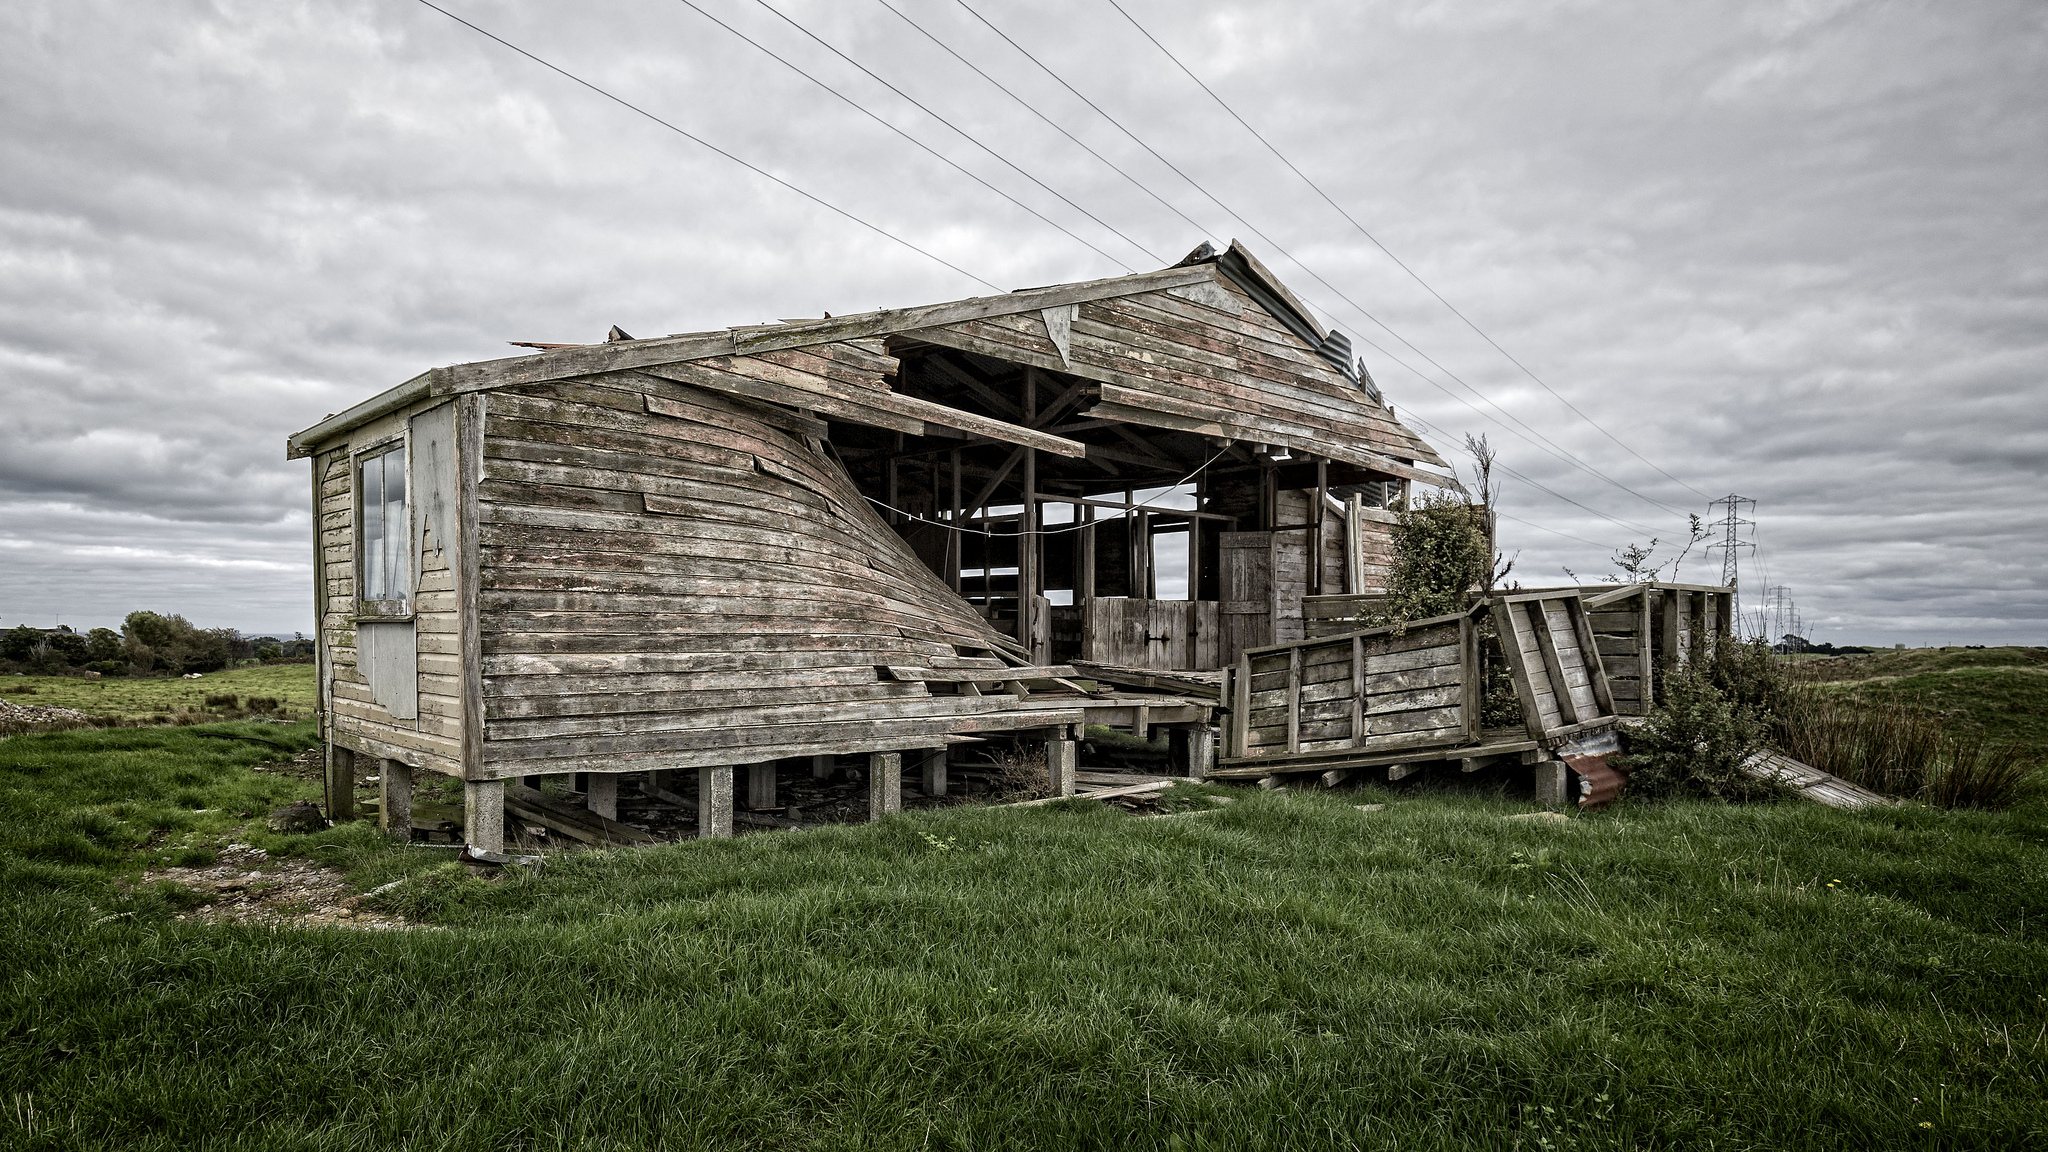
\includegraphics[width=0.8\textwidth]{figures/hut.jpg}
		\hspace*{15pt}\hbox{\scriptsize Image By:\thinspace{\itshape Dave Young}}
		% https://www.flickr.com/photos/dcysurfer/26103416154
	\end{center}
\end{frame}

\begin{frame}
	\frametitle{Can we do better?}
	\begin{columns}
		\column{0.705\textwidth}
	\begin{algorithmic}
		\State Sort all points by x-coordinate
		\Function{Closest-Pair}{$p_1,\dots,p_n$}
			\If{n=1}
				\State \Return $\infty$
			\EndIf
			\State $L \gets$ median $x$-coordinate
			\State $\delta_1 \gets$ \Call{Closest-Pair}{Points left of $L$}
			\State $\delta_2 \gets$ \Call{Closest-Pair}{Points right of $L$}
			\State $\delta \gets \min(\delta_1,\delta_2)$
			\State get list of all points within $\delta$ from L.
			\State \alert{sort this list by y-coordinate}
			\State Scan by y-order, compare every point to the next 11 and update $\delta$ as you go.
			\State \Return $\delta$
		\EndFunction
	\end{algorithmic}
		\column{0.205\textwidth}
		\pause
		\begin{questionblock}{}
			Do we need to sort every time?
		\end{questionblock}	
		\pause
		\begin{answerblock}{}
			No! How about just once before we start?
		\end{answerblock}
	\end{columns}
	
\end{frame}

\begin{frame}
	\frametitle{Back to closest pair of points}
	\section{Closest pair of points}
\label{sec:closest_pair_of_points}


\begin{frame}
	\frametitle{A new problem}
	\begin{problemblock}{Closest pair of points}
		Given a set of points, what is the pair of points that is closest to each other?\\
		\pause
		More formally:
		\begin{itemize}
			\item Given a set of points $S$, where every point $p_i$ has an x-coordinate $x_i$ and y-coordinate $y_i$.
			\item Distance is defined as: $d(i,j) = \sqrt{{(x_i - x_j)}^{2} + {(y_i-y_j)}^2}$
			\item What is the pair of points $i,j$ such that $d(i,j)$ is minimal?
		\end{itemize}
	\end{problemblock}
	\pause
	\section{Closest pair of points}
\label{sec:closest_pair_of_points}


\begin{frame}
	\frametitle{A new problem}
	\begin{problemblock}{Closest pair of points}
		Given a set of points, what is the pair of points that is closest to each other?\\
		\pause
		More formally:
		\begin{itemize}
			\item Given a set of points $S$, where every point $p_i$ has an x-coordinate $x_i$ and y-coordinate $y_i$.
			\item Distance is defined as: $d(i,j) = \sqrt{{(x_i - x_j)}^{2} + {(y_i-y_j)}^2}$
			\item What is the pair of points $i,j$ such that $d(i,j)$ is minimal?
		\end{itemize}
	\end{problemblock}
	\pause
	\input{figures/tikz/closestpair.tex}
	\pnote{Why is this relevant? Answers: For instance collision detection algorithms}
\end{frame}

\begin{frame}
	\frametitle{Let's just brute-force it?}
	\begin{overlayarea}{\textwidth}{\textheight}
		\input{figures/tikz/closestpair.tex}
		\begin{questionblock}{Brute-force}
			What is the tightest upper bound on the run time for a brute-force solution given $|S| = n$?
			\only<2>{
			\begin{enumerate}[A.]
				\item $O(n \log n)$
				\item $O(n^2)$
				\item $O(n^2 \log n)$
				\item $O(n^3)$
				\item I don't know.
			\end{enumerate}
		}
		\end{questionblock}
		\only<3>{
			\begin{answerblock}{Try every combination}
				We check every pair of points, of which there are $n^2$, so $O(n^2)$.	
			\end{answerblock}
		}
	\end{overlayarea}
\end{frame}

\begin{frame}
	\frametitle{Time to improve!}
	\framesubtitle{Using Divide \& Conquer}
		\begin{columns}
			\column{0.455\textwidth}
			\begin{center}
				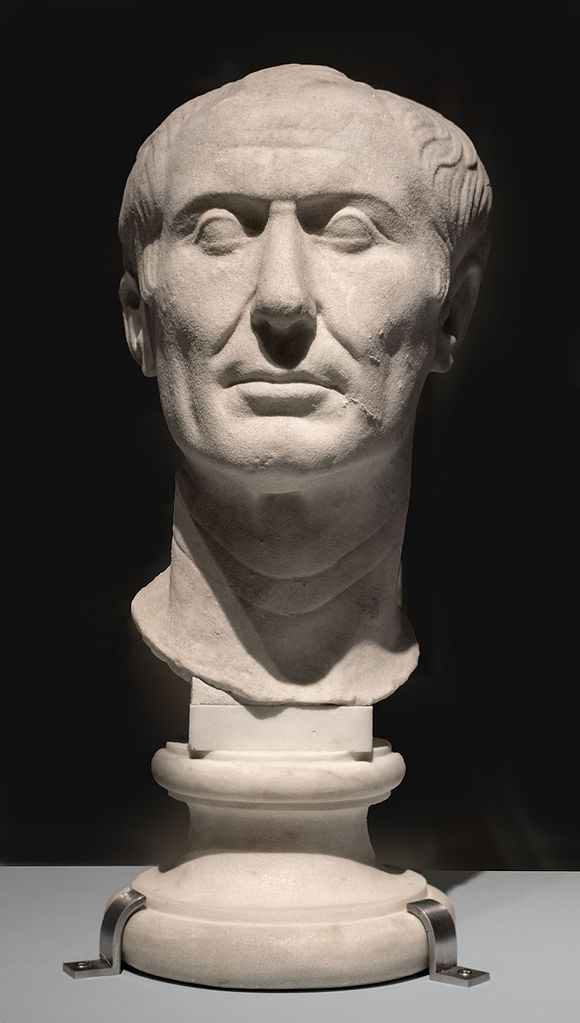
\includegraphics[width=0.5\textwidth]{figures/ceasar.jpg}\\
				\hspace*{15pt}\hbox{\scriptsize Image By:\thinspace{\itshape Ángel M. Felicísimo}}
				%https://commons.wikimedia.org/wiki/File:Retrato_de_Julio_C%C3%A9sar_(26724093101).jpg
			\end{center}

			\column{0.455\textwidth}
			\begin{center}
				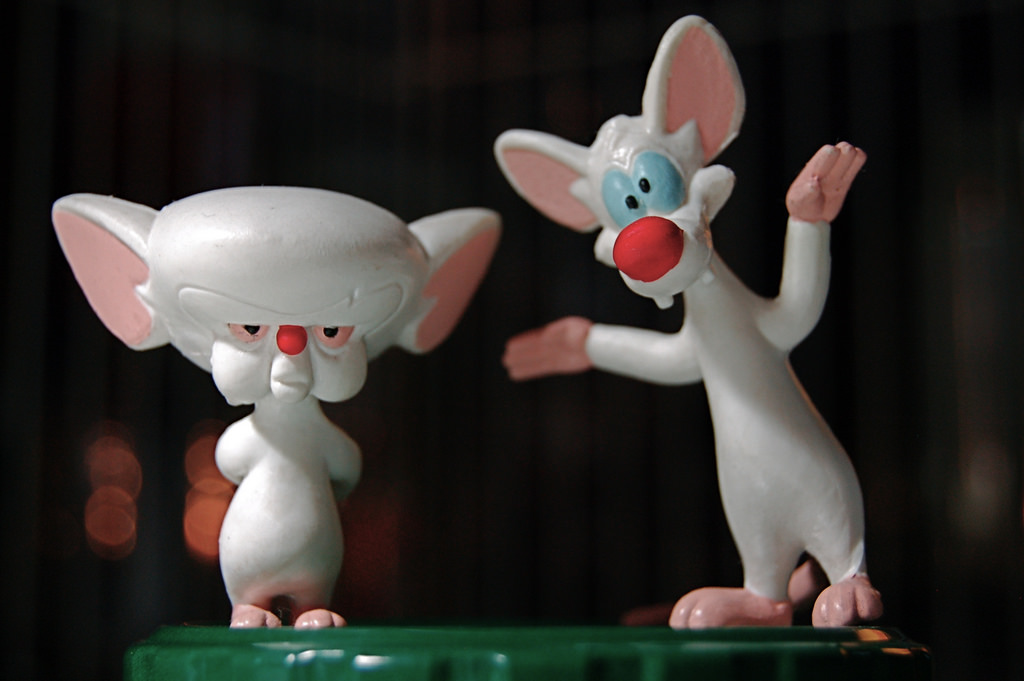
\includegraphics[width=0.9\textwidth]{figures/pinky.jpg}\\
				\hspace*{15pt}\hbox{\scriptsize Image By:\thinspace{\itshape JD Hancock}}
				%https://commons.wikimedia.org/wiki/File:Retrato_de_Julio_C%C3%A9sar_(26724093101).jpg

			\end{center}
		\end{columns}
\end{frame}

\begin{frame}
	\frametitle{Ideas for an algorithm}

	\begin{overlayarea}{\textwidth}{\textheight}
		\input{figures/tikz/closestpair_fixed.tex}
		
		\pause
		\begin{exampleblock}{Algorithm}
			\begin{itemize}
				\item \alert<2>{Divide}: Draw vertical line $L$ that has roughly half of the points on each side.
					\pause
				\item \alert<3>{Conquer}: Find the closest pair on each side.
					\pause
				\item \alert<4>{Combine}: Find the closest pair with one point on each side.
					\pause
				\item Return the minimum of these 3.
			\end{itemize}
		\end{exampleblock}	
	\end{overlayarea}
\end{frame}

\begin{frame}
	\frametitle{Did we make things better?}
	\begin{questionblock}{What is the run time of combine?}
		How much time to combine the two halves? Remember that we want to improve over $\Theta(n^2)$.
	\end{questionblock}	
\end{frame}

\begin{frame}
	\frametitle{How do we make it better?}
		\input{figures/tikz/closestpair_fixed2.tex}
	Observation:
	\begin{itemize}
		\item If $\delta$ is the minimum of the smallest distances left and right.
			\pause
		\item Then we only need to consider pairs of points within $\delta$ of $L$.
			\pause
		\item So in this example, none at all!
	\end{itemize}
\end{frame}

\begin{frame}
	\frametitle{Worst-case?}
	\begin{overlayarea}{\textwidth}{\textheight}
			\begin{itemize}
				\item But worst-case all points are in this $2\delta$-strip...
					\pause
				\item But if we sort them by $y$-coordinate (which can be done in $O(n\log n)$), then how many comparisons do we need?
					\pause
				\item Still $O(n^2)$!?
					\only<4->{
				\item Nope! We only need to check within 11 (i.e. a constant number of) positions in the sorted list.
				}
					\only<5->{
				\item So the combining step is $O(n \log n)$ (which can be further improved to $O(n)$)!
				}
			\end{itemize}
			\only<3>{
			\begin{center}
				
\includegraphics[width=0.4\textwidth]{figures/dilbert.jpg}
				\framesubtitle{http://thecontextofthings.com/wp-content/uploads/2017/11/dilbert-work.jpg}
			\end{center}
		}
	\end{overlayarea}
\end{frame}

\begin{frame}
	\frametitle{Why 11?}

	\begin{overlayarea}{\textwidth}{\textheight}
		\begin{columns}
			\column{0.655\textwidth}
			\begin{block}{Definition}
				Let $s_i$ be the point in the $2\delta$-strip with the $i^\text{th}$ smallest $y$-coordinate.
			\end{block}	
			
			\pause
			\begin{block}{Claim about 11}
				If $|i-j| > 11$ then the distance between $s_i$ and $s_j$ is at least $\delta$.
			\end{block}
			\column{0.255\textwidth}
			\input{figures/tikz/closestpair_delta.tex}	
		\end{columns}
		
		\pause
		\only<3-5>{
			\begin{block}{Proof sketch}
			\begin{itemize}
				\item No two points are in the same $0.5\delta$-by-$0.5\delta$-box.
					\only<4->{
				\item Two points that have two rows between them have a distance $\geq 2\cdot(0.5\delta) = \delta$.
				}
				\only<5->{
				\item So we only consider points at most 2 rows away.
				}
			\end{itemize}
		\end{block}
	}
	\only<6->{
		\begin{exampleblock}{Fun facts!}
			\begin{itemize}
				\item We can even reduce this to just 7 points.
					\only<7>{
				\item Even less if we consider columns separately.
				}
			\end{itemize}
		\end{exampleblock}	
	}
		
		\only<3>{
		\begin{questionblock}{Why not?}
			Why are there no two points in the same box?
		\end{questionblock}
}
	\end{overlayarea}
\end{frame}

\begin{frame}
	\frametitle{The algorithm}
	\begin{columns}
		\column{0.705\textwidth}
	\begin{algorithmic}
		\State Sort all points by x-coordinate
		\Function{Closest-Pair}{$p_1,\dots,p_n$}
			\If{n=1}
				\State \Return $\infty$
			\EndIf

			\pause
			\State $L \gets$ \alert<2>{median} $x$-coordinate
			\State $\delta_1 \gets$ \Call{Closest-Pair}{Points left of $L$}
			\State $\delta_2 \gets$ \Call{Closest-Pair}{Points right of $L$}
			\State $\delta \gets \min(\delta_1,\delta_2)$
			\pause
			\State get list of all points within $\delta$ from L.
			\State sort this list by y-coordinate
			\pause
			\State Scan by y-order, compare every point to the next 11 and update $\delta$ as you go.
			\State \Return $\delta$
		\EndFunction
	\end{algorithmic}
		\pnote{Why not the average?}
		\column{0.205\textwidth}
		\pause
		\begin{questionblock}{}
			What is the recurrence equation for the run time?	
		\end{questionblock}	
		\pause
		\begin{answerblock}{}
			\small
			$T(n) =2T(n/2) + O(n\log n)$	
		\end{answerblock}
	\end{columns}
	
\end{frame}

	\pnote{Why is this relevant? Answers: For instance collision detection algorithms}
\end{frame}

\begin{frame}
	\frametitle{Let's just brute-force it?}
	\begin{overlayarea}{\textwidth}{\textheight}
		\section{Closest pair of points}
\label{sec:closest_pair_of_points}


\begin{frame}
	\frametitle{A new problem}
	\begin{problemblock}{Closest pair of points}
		Given a set of points, what is the pair of points that is closest to each other?\\
		\pause
		More formally:
		\begin{itemize}
			\item Given a set of points $S$, where every point $p_i$ has an x-coordinate $x_i$ and y-coordinate $y_i$.
			\item Distance is defined as: $d(i,j) = \sqrt{{(x_i - x_j)}^{2} + {(y_i-y_j)}^2}$
			\item What is the pair of points $i,j$ such that $d(i,j)$ is minimal?
		\end{itemize}
	\end{problemblock}
	\pause
	\input{figures/tikz/closestpair.tex}
	\pnote{Why is this relevant? Answers: For instance collision detection algorithms}
\end{frame}

\begin{frame}
	\frametitle{Let's just brute-force it?}
	\begin{overlayarea}{\textwidth}{\textheight}
		\input{figures/tikz/closestpair.tex}
		\begin{questionblock}{Brute-force}
			What is the tightest upper bound on the run time for a brute-force solution given $|S| = n$?
			\only<2>{
			\begin{enumerate}[A.]
				\item $O(n \log n)$
				\item $O(n^2)$
				\item $O(n^2 \log n)$
				\item $O(n^3)$
				\item I don't know.
			\end{enumerate}
		}
		\end{questionblock}
		\only<3>{
			\begin{answerblock}{Try every combination}
				We check every pair of points, of which there are $n^2$, so $O(n^2)$.	
			\end{answerblock}
		}
	\end{overlayarea}
\end{frame}

\begin{frame}
	\frametitle{Time to improve!}
	\framesubtitle{Using Divide \& Conquer}
		\begin{columns}
			\column{0.455\textwidth}
			\begin{center}
				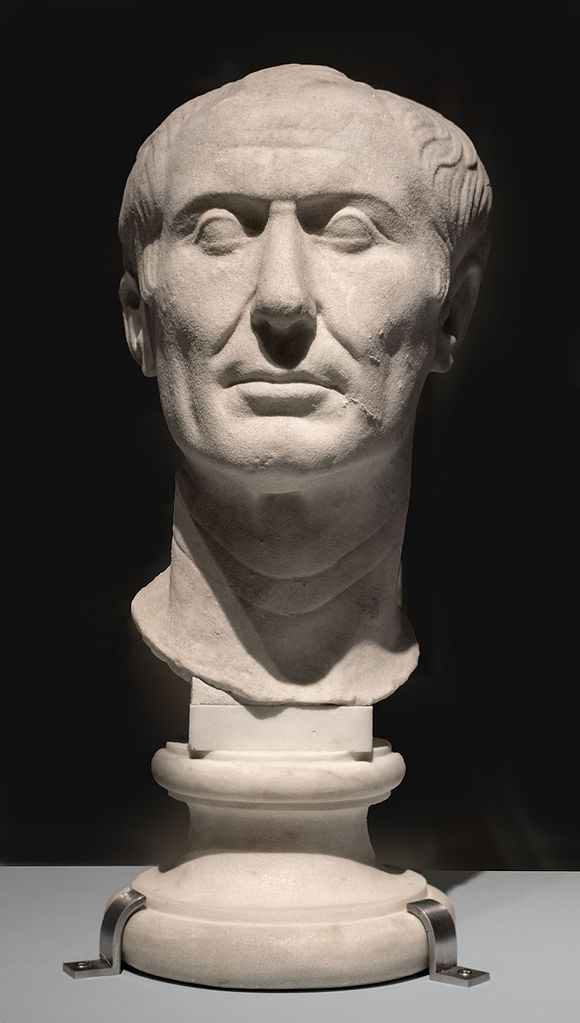
\includegraphics[width=0.5\textwidth]{figures/ceasar.jpg}\\
				\hspace*{15pt}\hbox{\scriptsize Image By:\thinspace{\itshape Ángel M. Felicísimo}}
				%https://commons.wikimedia.org/wiki/File:Retrato_de_Julio_C%C3%A9sar_(26724093101).jpg
			\end{center}

			\column{0.455\textwidth}
			\begin{center}
				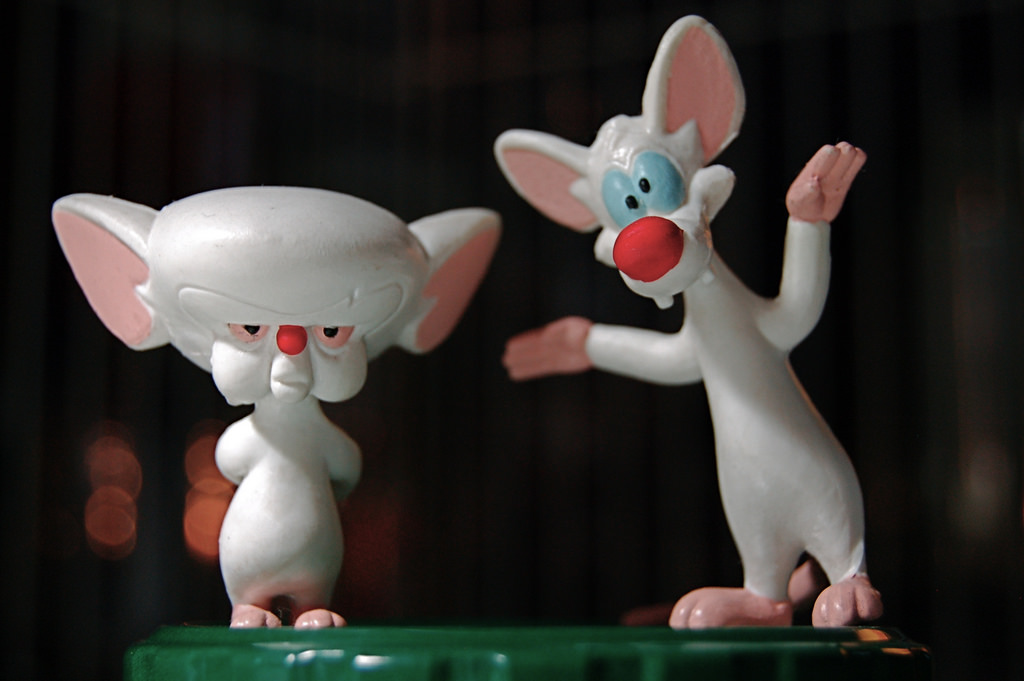
\includegraphics[width=0.9\textwidth]{figures/pinky.jpg}\\
				\hspace*{15pt}\hbox{\scriptsize Image By:\thinspace{\itshape JD Hancock}}
				%https://commons.wikimedia.org/wiki/File:Retrato_de_Julio_C%C3%A9sar_(26724093101).jpg

			\end{center}
		\end{columns}
\end{frame}

\begin{frame}
	\frametitle{Ideas for an algorithm}

	\begin{overlayarea}{\textwidth}{\textheight}
		\input{figures/tikz/closestpair_fixed.tex}
		
		\pause
		\begin{exampleblock}{Algorithm}
			\begin{itemize}
				\item \alert<2>{Divide}: Draw vertical line $L$ that has roughly half of the points on each side.
					\pause
				\item \alert<3>{Conquer}: Find the closest pair on each side.
					\pause
				\item \alert<4>{Combine}: Find the closest pair with one point on each side.
					\pause
				\item Return the minimum of these 3.
			\end{itemize}
		\end{exampleblock}	
	\end{overlayarea}
\end{frame}

\begin{frame}
	\frametitle{Did we make things better?}
	\begin{questionblock}{What is the run time of combine?}
		How much time to combine the two halves? Remember that we want to improve over $\Theta(n^2)$.
	\end{questionblock}	
\end{frame}

\begin{frame}
	\frametitle{How do we make it better?}
		\input{figures/tikz/closestpair_fixed2.tex}
	Observation:
	\begin{itemize}
		\item If $\delta$ is the minimum of the smallest distances left and right.
			\pause
		\item Then we only need to consider pairs of points within $\delta$ of $L$.
			\pause
		\item So in this example, none at all!
	\end{itemize}
\end{frame}

\begin{frame}
	\frametitle{Worst-case?}
	\begin{overlayarea}{\textwidth}{\textheight}
			\begin{itemize}
				\item But worst-case all points are in this $2\delta$-strip...
					\pause
				\item But if we sort them by $y$-coordinate (which can be done in $O(n\log n)$), then how many comparisons do we need?
					\pause
				\item Still $O(n^2)$!?
					\only<4->{
				\item Nope! We only need to check within 11 (i.e. a constant number of) positions in the sorted list.
				}
					\only<5->{
				\item So the combining step is $O(n \log n)$ (which can be further improved to $O(n)$)!
				}
			\end{itemize}
			\only<3>{
			\begin{center}
				
\includegraphics[width=0.4\textwidth]{figures/dilbert.jpg}
				\framesubtitle{http://thecontextofthings.com/wp-content/uploads/2017/11/dilbert-work.jpg}
			\end{center}
		}
	\end{overlayarea}
\end{frame}

\begin{frame}
	\frametitle{Why 11?}

	\begin{overlayarea}{\textwidth}{\textheight}
		\begin{columns}
			\column{0.655\textwidth}
			\begin{block}{Definition}
				Let $s_i$ be the point in the $2\delta$-strip with the $i^\text{th}$ smallest $y$-coordinate.
			\end{block}	
			
			\pause
			\begin{block}{Claim about 11}
				If $|i-j| > 11$ then the distance between $s_i$ and $s_j$ is at least $\delta$.
			\end{block}
			\column{0.255\textwidth}
			\input{figures/tikz/closestpair_delta.tex}	
		\end{columns}
		
		\pause
		\only<3-5>{
			\begin{block}{Proof sketch}
			\begin{itemize}
				\item No two points are in the same $0.5\delta$-by-$0.5\delta$-box.
					\only<4->{
				\item Two points that have two rows between them have a distance $\geq 2\cdot(0.5\delta) = \delta$.
				}
				\only<5->{
				\item So we only consider points at most 2 rows away.
				}
			\end{itemize}
		\end{block}
	}
	\only<6->{
		\begin{exampleblock}{Fun facts!}
			\begin{itemize}
				\item We can even reduce this to just 7 points.
					\only<7>{
				\item Even less if we consider columns separately.
				}
			\end{itemize}
		\end{exampleblock}	
	}
		
		\only<3>{
		\begin{questionblock}{Why not?}
			Why are there no two points in the same box?
		\end{questionblock}
}
	\end{overlayarea}
\end{frame}

\begin{frame}
	\frametitle{The algorithm}
	\begin{columns}
		\column{0.705\textwidth}
	\begin{algorithmic}
		\State Sort all points by x-coordinate
		\Function{Closest-Pair}{$p_1,\dots,p_n$}
			\If{n=1}
				\State \Return $\infty$
			\EndIf

			\pause
			\State $L \gets$ \alert<2>{median} $x$-coordinate
			\State $\delta_1 \gets$ \Call{Closest-Pair}{Points left of $L$}
			\State $\delta_2 \gets$ \Call{Closest-Pair}{Points right of $L$}
			\State $\delta \gets \min(\delta_1,\delta_2)$
			\pause
			\State get list of all points within $\delta$ from L.
			\State sort this list by y-coordinate
			\pause
			\State Scan by y-order, compare every point to the next 11 and update $\delta$ as you go.
			\State \Return $\delta$
		\EndFunction
	\end{algorithmic}
		\pnote{Why not the average?}
		\column{0.205\textwidth}
		\pause
		\begin{questionblock}{}
			What is the recurrence equation for the run time?	
		\end{questionblock}	
		\pause
		\begin{answerblock}{}
			\small
			$T(n) =2T(n/2) + O(n\log n)$	
		\end{answerblock}
	\end{columns}
	
\end{frame}

		\begin{questionblock}{Brute-force}
			What is the tightest upper bound on the run time for a brute-force solution given $|S| = n$?
			\only<2>{
			\begin{enumerate}[A.]
				\item $O(n \log n)$
				\item $O(n^2)$
				\item $O(n^2 \log n)$
				\item $O(n^3)$
				\item I don't know.
			\end{enumerate}
		}
		\end{questionblock}
		\only<3>{
			\begin{answerblock}{Try every combination}
				We check every pair of points, of which there are $n^2$, so $O(n^2)$.	
			\end{answerblock}
		}
	\end{overlayarea}
\end{frame}

\begin{frame}
	\frametitle{Time to improve!}
	\framesubtitle{Using Divide \& Conquer}
		\begin{columns}
			\column{0.455\textwidth}
			\begin{center}
				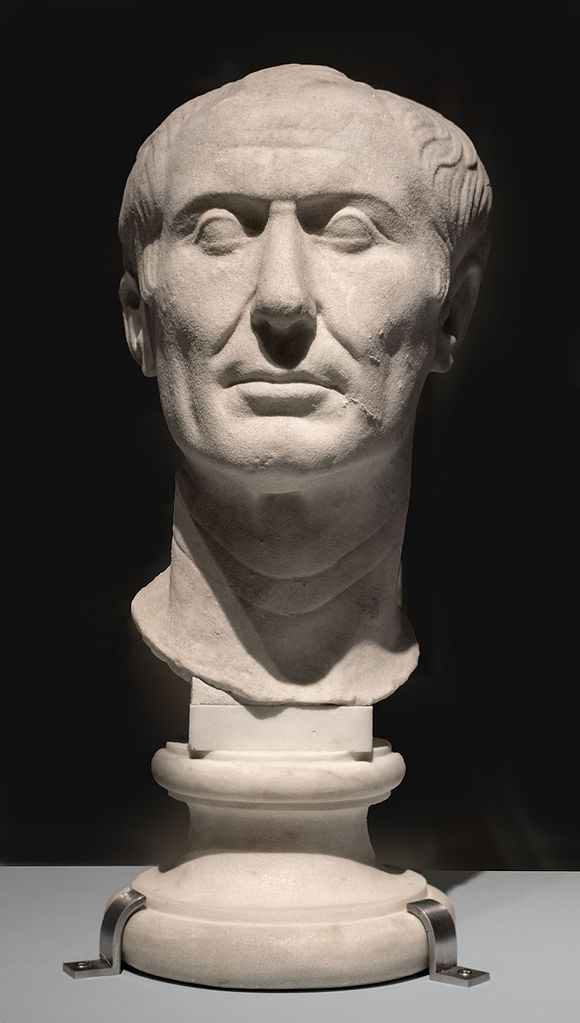
\includegraphics[width=0.5\textwidth]{figures/ceasar.jpg}\\
				\hspace*{15pt}\hbox{\scriptsize Image By:\thinspace{\itshape Ángel M. Felicísimo}}
				%https://commons.wikimedia.org/wiki/File:Retrato_de_Julio_C%C3%A9sar_(26724093101).jpg
			\end{center}

			\column{0.455\textwidth}
			\begin{center}
				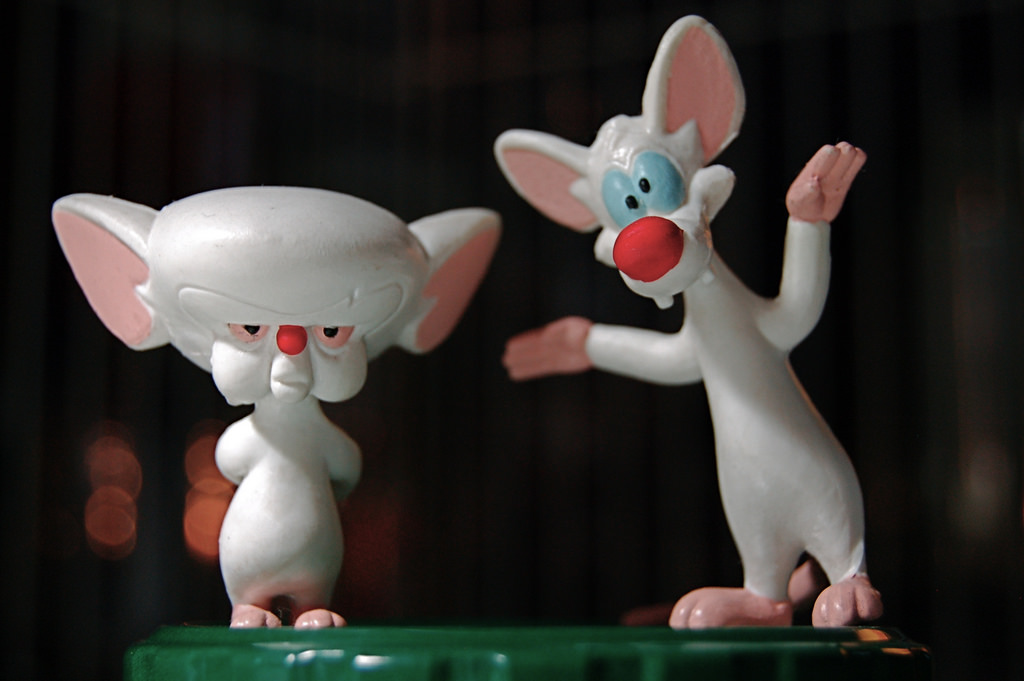
\includegraphics[width=0.9\textwidth]{figures/pinky.jpg}\\
				\hspace*{15pt}\hbox{\scriptsize Image By:\thinspace{\itshape JD Hancock}}
				%https://commons.wikimedia.org/wiki/File:Retrato_de_Julio_C%C3%A9sar_(26724093101).jpg

			\end{center}
		\end{columns}
\end{frame}

\begin{frame}
	\frametitle{Ideas for an algorithm}

	\begin{overlayarea}{\textwidth}{\textheight}
		\begin{figure}[htpb]
\begin{center}
\begin{tikzpicture}[scale=0.5, transform shape]
	\draw (-8,-3) rectangle (8,3);

	\foreach \x/\y/\name in {
		-7/2/,
		-6/1/l1,
		-5/1/l2,
		-3/-2/c1,
		-1/-2/c2,
		3/-1/,
		5/1.5/r1,
		5/0/r2,
		}{
		\node[circle, black, draw, fill=blue!30, minimum size=4pt] (\name) at (\x,\y) {};
	}
		\node at (-1.5, -3.5) {};
	\only<2->{
		\draw[dotted] (-1.5,-3) -- (-1.5,3);
		\node at (-1.5, -3.5) {\Large $L$};
	}
	\only<3->{
		\draw[dotted, red, thick] (l1) --  node[anchor=south] {\Large 1} (l2);
		\draw[dotted, red, thick] (r1) --  node[anchor=west] {\Large 1.5} (r2);
	}
	\only<4->{
		\draw[dotted, red, thick] (c1) --  node[anchor=south] {\Large 2} (c2);
	}
\end{tikzpicture}
\end{center}
\end{figure}

		
		\pause
		\begin{exampleblock}{Algorithm}
			\begin{itemize}
				\item \alert<2>{Divide}: Draw vertical line $L$ that has roughly half of the points on each side.
					\pause
				\item \alert<3>{Conquer}: Find the closest pair on each side.
					\pause
				\item \alert<4>{Combine}: Find the closest pair with one point on each side.
					\pause
				\item Return the minimum of these 3.
			\end{itemize}
		\end{exampleblock}	
	\end{overlayarea}
\end{frame}

\begin{frame}
	\frametitle{Did we make things better?}
	\begin{questionblock}{What is the run time of combine?}
		How much time to combine the two halves? Remember that we want to improve over $\Theta(n^2)$.
	\end{questionblock}	
\end{frame}

\begin{frame}
	\frametitle{How do we make it better?}
		\begin{figure}[htpb]
\begin{center}
\begin{tikzpicture}[scale=0.5, transform shape]
	\draw (-8,-3) rectangle (8,3);

	\only<2->{
		\draw[fill=gray!10] (-2.5,-3) rectangle (-0.5,3);
	}
	\foreach \x/\y/\name in {
		-7/2/,
		-6/1/l1,
		-5/1/l2,
		-3/-2/c1,
		-1/-2/c2,
		3/-1/,
		5/1.5/r1,
		5/0/r2,
		}{
		\node[circle, black, draw, fill=blue!30, minimum size=4pt] (\name) at (\x,\y) {};
	}
		\draw[dotted] (-1.5,-3) -- (-1.5,3);
		\node at (-1.5, -3.5) {\Large $L$};
		\draw[dotted, red, thick] (l1) --  node[anchor=south] {\Large 1} (l2);
		\draw[dotted, red, thick] (r1) --  node[anchor=west] {\Large 1.5} (r2);
		\draw[dotted, red, thick] (c1) --  node[anchor=south] {\Large 2} (c2);

\end{tikzpicture}
\end{center}
\end{figure}

	Observation:
	\begin{itemize}
		\item If $\delta$ is the minimum of the smallest distances left and right.
			\pause
		\item Then we only need to consider pairs of points within $\delta$ of $L$.
			\pause
		\item So in this example, none at all!
	\end{itemize}
\end{frame}

\begin{frame}
	\frametitle{Worst-case?}
	\begin{overlayarea}{\textwidth}{\textheight}
			\begin{itemize}
				\item But worst-case all points are in this $2\delta$-strip...
					\pause
				\item But if we sort them by $y$-coordinate (which can be done in $O(n\log n)$), then how many comparisons do we need?
					\pause
				\item Still $O(n^2)$!?
					\only<4->{
				\item Nope! We only need to check within 11 (i.e. a constant number of) positions in the sorted list.
				}
					\only<5->{
				\item So the combining step is $O(n \log n)$ (which can be further improved to $O(n)$)!
				}
			\end{itemize}
			\only<3>{
			\begin{center}
				
\includegraphics[width=0.4\textwidth]{figures/dilbert.jpg}
				\framesubtitle{http://thecontextofthings.com/wp-content/uploads/2017/11/dilbert-work.jpg}
			\end{center}
		}
	\end{overlayarea}
\end{frame}

\begin{frame}
	\frametitle{Why 11?}

	\begin{overlayarea}{\textwidth}{\textheight}
		\begin{columns}
			\column{0.655\textwidth}
			\begin{block}{Definition}
				Let $s_i$ be the point in the $2\delta$-strip with the $i^\text{th}$ smallest $y$-coordinate.
			\end{block}	
			
			\pause
			\begin{block}{Claim about 11}
				If $|i-j| > 11$ then the distance between $s_i$ and $s_j$ is at least $\delta$.
			\end{block}
			\column{0.255\textwidth}
			\begin{figure}[htpb]
\begin{center}
\begin{tikzpicture}[scale=0.4, transform shape]
	\draw (-2,-4) rectangle (2,4);
	
	\only<5->{
		\foreach \y in {-2, ..., 0}{
			\foreach \x in {-2, ..., 1}{
				\draw[fill=green!30] (\x,\y) rectangle (\x+1,\y+1);
			}
		}
	}

	\foreach \x/\y/\name/\color in {
		1.35/-2.4/1/red,
		-1.35/-1.6/2/green,
		-0.4/-0.4/3/blue,
		1.3/0.5/4/blue,
	%	1.7/1.4/5/red,
		-0.4/2.4/5/red,
		0.3/2.4/6/red}{
		\alt<4->{
		\node[circle, black, draw, fill=\color!30, minimum size=4pt] () at (\x,\y) {\name};
			}{
		\node[circle, black, draw, fill=blue!30, minimum size=4pt] () at (\x,\y) {\name};
		}
	}
		\draw[thick] (0,-4) -- (0,4);
		\node at (0, -4.5) {\Large $L$};
		\node at (-2, -4.5) {\Large $L-\delta$};
		\node at (2, -4.5) {\Large $L+\delta$};
		\only<3->{
			\draw[dotted] (1,-4) -- (1,4);
			\draw[dotted] (-1,-4) -- (-1,4);

			\foreach \y in {-3, ..., 3}{
				\draw[dotted] (-2,\y) -- (2,\y);
			}
		}

\end{tikzpicture}
\end{center}
\end{figure}
	
		\end{columns}
		
		\pause
		\only<3-5>{
			\begin{block}{Proof sketch}
			\begin{itemize}
				\item No two points are in the same $0.5\delta$-by-$0.5\delta$-box.
					\only<4->{
				\item Two points that have two rows between them have a distance $\geq 2\cdot(0.5\delta) = \delta$.
				}
				\only<5->{
				\item So we only consider points at most 2 rows away.
				}
			\end{itemize}
		\end{block}
	}
	\only<6->{
		\begin{exampleblock}{Fun facts!}
			\begin{itemize}
				\item We can even reduce this to just 7 points.
					\only<7>{
				\item Even less if we consider columns separately.
				}
			\end{itemize}
		\end{exampleblock}	
	}
		
		\only<3>{
		\begin{questionblock}{Why not?}
			Why are there no two points in the same box?
		\end{questionblock}
}
	\end{overlayarea}
\end{frame}

\begin{frame}
	\frametitle{The algorithm}
	\begin{columns}
		\column{0.705\textwidth}
	\begin{algorithmic}
		\State Sort all points by x-coordinate
		\Function{Closest-Pair}{$p_1,\dots,p_n$}
			\If{n=1}
				\State \Return $\infty$
			\EndIf

			\pause
			\State $L \gets$ \alert<2>{median} $x$-coordinate
			\State $\delta_1 \gets$ \Call{Closest-Pair}{Points left of $L$}
			\State $\delta_2 \gets$ \Call{Closest-Pair}{Points right of $L$}
			\State $\delta \gets \min(\delta_1,\delta_2)$
			\pause
			\State get list of all points within $\delta$ from L.
			\State sort this list by y-coordinate
			\pause
			\State Scan by y-order, compare every point to the next 11 and update $\delta$ as you go.
			\State \Return $\delta$
		\EndFunction
	\end{algorithmic}
		\pnote{Why not the average?}
		\column{0.205\textwidth}
		\pause
		\begin{questionblock}{}
			What is the recurrence equation for the run time?	
		\end{questionblock}	
		\pause
		\begin{answerblock}{}
			\small
			$T(n) =2T(n/2) + O(n\log n)$	
		\end{answerblock}
	\end{columns}
	
\end{frame}

	\begin{problemblock}{The recurrence equation}
		\small
		$T(n) =2T(n/2) + O(n)$	\\
		\only<1>{
		Which part of the algorithm uses strictly more time?
		\begin{enumerate}[A.]
			\item Work in the leaves: $n^{\log_b a}$.
			\item Work in the root node: $f(n)$.
			\item Evenly spread throughout the tree.
			\item We cannot apply the master method.
		\end{enumerate}
	}
	\end{problemblock}

	\pause
	\begin{answerblock}{Case ...?}
		\small
		$a = 2, b =2, n^{\log_b a} = n^{\log_2 2} = n^1$\\
		$f(n)$ is $\Theta(n)$\\
		So case 2 of the master method (work is evenly spread)
	\end{answerblock}
\end{frame}

\begin{frame}
	\frametitle{You are here.}
	\begin{block}{The course so far}
		\begin{itemize}
			\item Time and Space complexity
			\item Lists, Stacks, and Queues
			\item Sorting
		\end{itemize}
	\end{block}
	\pause
	\begin{exampleblock}{Today's content}
		\begin{itemize}
			\item Trees!
			\item Properties and traversals
		\end{itemize}
	\end{exampleblock}
	\pause
	\begin{block}{The future}
		\begin{itemize}
			\item Heaps and Search Trees
			\item Maps, Sets, and Graphs
			\item P vs NP\dots
		\end{itemize}
	\end{block}
\end{frame}

\begin{frame}
	\frametitle{Homework for this week}
	\begin{itemize}[<+->]
		\item \alert{After} today's lecture: read the Chapter 8.
		\item \alert{Before} Friday, check out the example exam (so that you can ask questions).
		\item \alert{Before} Sunday, do the homework :)
	\end{itemize}
\end{frame}

\begin{frame}
	\frametitle{Mudcards}
	\framesubtitle{\url{https://www.delta.tudelft.nl/article/column-van-koelkasten-kranen-en-college}}

	\begin{block}{Based on a column by Bob van Vliet}
		\begin{itemize}
			\item At the end of every lecture, a short (2-question) survey.
			\item Tell me one thing you liked.
			\item And one thing you didn't like.
			\item Be concrete, be specific!
		\end{itemize}
	\end{block}
\end{frame}



\frame{\titlepage}

\end{document}
